%%%
%%% OpenCAEシンポジウムTeXテンプレートファイル
%%% OpenFAOM-jp_OpenCAE_symposium.tex
%%% OpenCAEシンポジウム2018版
%%%
%%
%% ltjocはOpenCAE論文集・シンポジウム用のクラスファイルです.変更しないでください.
%% 本文が英語の場合には,オプションにenglishを指定してください.
\documentclass{ltjoc}
%\documentclass[english]{ltjoc}
\usepackage[
 backgroundcolor=gray!50,
 usernamecolor=black,
 machinenamecolor=black,
 indicatorcolor=black,
 separatorcolor=black,
 pathcolor=black,
 optioncolor=black,
 textcolor=black
]{shdoc}
%%
%% 表題(title),副題(subtitle),著者(author),所属(affiliation)
%% 本文が英語の場合には,こちらに英文表題,英文副題,英文著者,英文所属を記述します.
\title{OpenFOAMコントリビュート活動}
% 副題が無い場合にはコメントアウトします.
% \subtitle{\TeX のテンプレート(和文副題)} 
\author{%
稲葉竜一$^{1\dagger}$%
\hspace{1\zw}%
松原 大輔$^{2}$%
\hspace{1\zw}%
@tkoyama010$^{1}$%
}
\affiliation{%
${}^{1}$OpenFOAM-jp%
\hspace{1\zw}%
${}^{2}$オープン CAE勉強会%
} 
%%
%% Corresponding authorの電子メールアドレス
%% 本論文について連絡が取れる著者の電子メールアドレスを記載してください.
\AuthorsEmail{inabower@gmail.co.jp}
%%
%% 英文表題(etitle),英文副題(esubtitle),英文著者(eauthor),英文所属(eaffiliation)
%% 本文が英語の場合には表示されません.
\etitle{OpenFOAM Contributing Activities}
% 副題が無い場合にはコメントアウトします.
% \esubtitle{The case of \TeX (English Sub-Title)}
\eauthor{%
Ryuichi INABA$^{*\dagger}$%
\hspace{1em}%
Daisuke MATSUBARA$^{**}$%
\hspace{1em}%
@tkoyama010$^{*}$%
}
\eaffiliation{%
${}^{*}$OpenFOAM-jp%
\hspace{1em}%
${}^{**}$OpenCAE Local user group%
}
%%
%% キーワード
\keywords{GitHub, git, Pull Request, OpenFOAM, develop}
%%
%% 英文概要
%% 英文概要を省略する場合には,abstract環境の定義をしないでください.
\begin{abstract}

\end{abstract}
%%
%% luatexja-fontspecパッケージ
\usepackage{luatexja-fontspec}
\defaultfontfeatures{Ligatures=TeX}
%% luatexja-presetパッケージ
%% 和文フォントのプリセット設定
%% オプションにnoembed(非埋込)を指定しないでください.
%\usepackage[ipaex]{luatexja-preset} % IPAex(デフォルト)
%\usepackage[ms]{luatexja-preset} % MS
%\usepackage[hiragino-pro]{luatexja-preset} % ヒラギノPro
%%
%% 欧文フォントの指定
%% 使用できるフォントについては,以下のコマンドで調べてください.
%% $ luaotfload-tool --list=*
%%
%% 欧文通常フォント
%\setmainfont{Cambria} % Cambria
%\setmainfont{Times New Roman} % Times New Roman
%\setmainfont{TeXGyreTermes} % TeXGyreTermes
%%
%% 欧文Sans-serifフォント
%\setsansfont{Calibri} % Calibri
%\setsansfont{Arial} % Arial
%\setsansfont{Helvetica} % Helvetica
%\setsansfont{TeXGyreHeros} % TeXGyreHeros
%%
%% 欧文monospaceフォント
%\setmonofont{Consolas} % Consolas
%\setmonofont{Courier New} % Courier New
%\setmonofont{Lucida Console} % Lucida Console
%%
%% subfigureパッケージ
\usepackage{subfigure}
%%
%% graphicxパッケージ
\usepackage{graphicx}
%%
%% hyperrefパッケージ
\usepackage[
 pdfencoding=auto,
 bookmarks=true,
 bookmarksnumbered=true,
 colorlinks=true,
 allcolors={blue}
]{hyperref}
%%
%% listingsパッケージ
\usepackage{listings}
\renewcommand{\lstlistingname}{Code}
\lstset{
basicstyle={\footnotesize\ttfamily},
commentstyle=\color{blue},
frame={tb},
breaklines=true,
columns=[l]{fullflexible},
numbers=left,
numberstyle={\footnotesize},
keepspaces=true
}
%%
%% autorefでの図表の参照名の再定義
\makeatletter
\if@english
  \renewcommand*{\figureautorefname}{\figurename}
  \renewcommand*{\tableautorefname}{\tablename}
\else
  \renewcommand*{\figureautorefname}{図}
  \renewcommand*{\tableautorefname}{表}
\fi
\makeatother
%%
%% ヘッダ右の設定
%% 変更しないでください.
\markright{Open CAE Symposium 2019, Dec. 19-21, 2019, Osaka, D-2} % Do not edit this line
%%
%% 本文
\begin{document}
%%
%% 題目などの出力
\maketitle
%%%
\section{はじめに}
現状日本からのOpenFOAMへのコントリビュートは少ない.
そこで有志により"OpenFOAM-jp"というグループを立ち上げ,本家の開発やドキュメントの翻訳,チュートリアルの作成などのコントリビュート活動を始めた.
本報告ではその活動内容などについて発表する.
\section{Foundation版とESI版の違い}
OpenFOAMは,Imperial Collageで開発された商用CFDコードFOAM(Field Operation And Manipulation)が,2004年にOpenFOAMと名前を変えてオープンソースとしてリリースされたことから始まる.\cite{URL:openfoam.history}\cite{Minabe:OpenCAE2015-GP23}
2011年にはOpenFOAMを運営しているOpenCFD社がSGI社に買収され,またその2社によりOpenFOAMの商標を譲渡したOpenFOAM Foundation Inc.を設立した.
これ以降OpenFOAMはOpenFOAM Foundation Inc.より開発と配布が行われており,2019年11月現在OpenFOAM-V7を最新版とするForkが”Foundation版”\cite{URL:openfoam.org}\cite{URL:GitHub-foundation}と呼ばれている.

一方でOpenFOAMには多くのForkが存在する.
2012年以降はESI社がOpenCFD社の買収という形から開発に加わるようになり,
2016年にはOpenFOAM-v3.0からForkしたOpenFOAM-v3.0+をリリースした.
2019年11月時点ではこの最新版はOpenFOAM-v1906であり,このForkが”ESI版”\cite{URL:openfoam.com}\cite{URL:GitLab-plus}もしくは”plus版”と呼ばれる.

本報告ではこのFoudation版とESI版の2つについてコントリビュートの流れなどを報告する.
%
\section{ESI版コントリビュート方法}
ESI版の開発はGitLabで行われている.\cite{URL:GitLab-plus}
このページからレポジトリをcloneすることができ,これをそのままコンパイルすることで次期リリース予定のESI版OpenFOAMを使用することができる.
またここには開発途中のbranchが多くあり,将来的に追加されるであろう機能をチェックすることもできる.

\autoref{fig:plus-register}に示すGitLabのページの右上のボタンからこのOpenFOAM-plusのレポジトリに登録することもでき,これによりissueの作成や書き込みをすることができるようになる.
\begin{figure}[htbp]
\centering
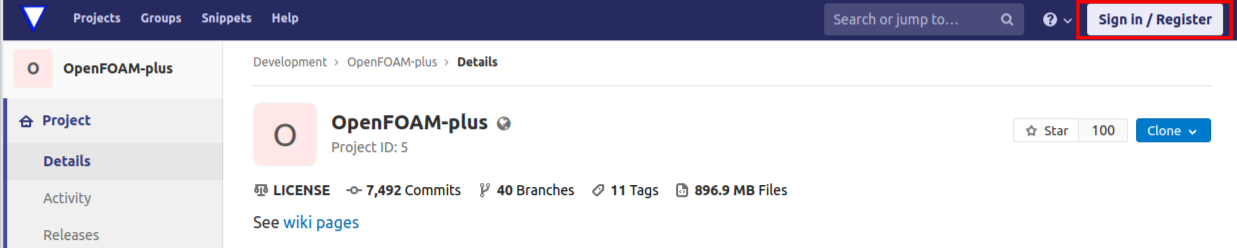
\includegraphics[width=0.8\textwidth]{fig/plus_register.png}
\caption{A register button of OpenFOAM-plus's GitLab page.}
\label{fig:plus-register}
\end{figure}
例えばバグを見つけた場合やOpenFOAMへの要望がある場合には,issueを作成することで開発者へ周知することができ,必要と判断された場合には開発者によりコードの修正や作成が行われる.
\autoref{fig:plus-issue}には実際に作成したissueの例を示す.内容としてはソルバーのDiscriptionの中のスペルミスを指摘した簡単なものであるが,数日以内に@mark氏により該当箇所の修正が行われていることが確認できる.
\begin{figure}[htbp]
\centering
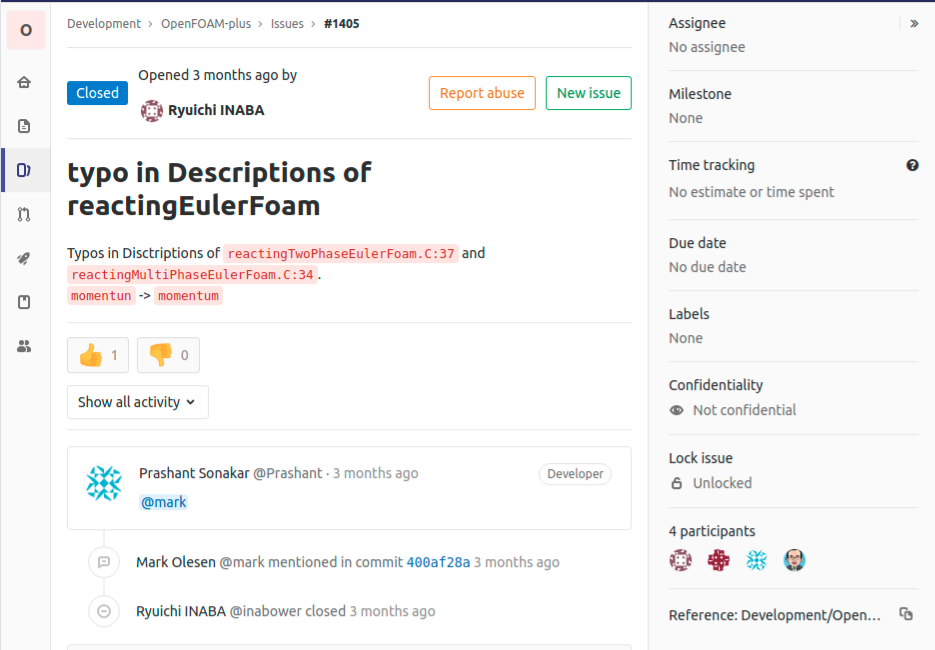
\includegraphics[width=0.8\textwidth]{fig/plus_issue.png}
\caption{An Example issue to fix typo.}
\label{fig:plus-issue}
\end{figure}
このような小さなコントリビュートの積み重ねがOSSであるOpenFOAMを精錬していくこととなる.

一方で,pushやPull Requestなどのコードの変更を行うための権限は制限されている.
このため,ESI版OpenFOAMのコードにコントリビュートする手段としては,開発メンバーに加わらない限りはissueの作成もしくはissue内の議論へ参加することに限られる.
なお2019年11月現在OpenFOAM-plusの開発メンバーは15名であり,実力や面識,貢献頻度が担保されたメンバーで開発を行っていることが推察される.\cite{URL:GitLab-plus-members}
%
\section{Foundation版コントリビュート方法}

Foundation版の開発はGithubで行われている.Foundation版ではissueの管理はGithubでは行わないので注意が必要である.バグ報告は専用のissueTrackingのページへ登録する必要がある.
未登録の場合は,名前とメールアドレスを入力し,返信のリンクを辿ることでviewerとして参加することができる.
また数時間後にスパムでないことが認められると,reporterに昇格できる.
reporterとなることでissueを立てて,バグの報告が可能となる.
ここでバグの重要度や改善方法を議論をすることになる.
issueTrackingの内容を確認すると,Foundation版は基本的にbugfixを目的としたコントリビュートが主の様である.

重大なバグの修正または,新しい開発を提供する場合,OpenFOAM Foundation Contributor Agreementに署名する必要がある.
Foundation版HPのメニューバーのDevelopment/ContributorAgreeementのリンクを辿り,Contact Usのページから名前と所属,コントリビュートに参加した意思を記載して送信すると,後日,Henry G. WellerからPDF形式の登録用紙が送付されてくる.
登録用紙の内容は,前述のContributorAgreeementのページに記載されているものと同じである.

バグの修正などでFoundation版のOpenFOAMの修正を開発元に共有する場合,Foundation版のOpenFOAMはgithub上で管理されているため,githubアカウントが必要となる.

コントリビュートで最初に行うことは開発元のリポジトリをForkすることから始まる.(\autoref{fig:f1})
Forkしたことにより,自身のgithubアカウントにOpenFOAMのリポジトリが作成されていることが確認できる.
次に開発用の新しいブランチを作成する.ブランチ名は「(開発者名)-patch***」などとするとよいだろう.今回の例では「matsubara-patch1」とした.(\autoref{fig:f2})

\begin{figure}[htbp]
\centering
\subfigure[A fork button of Github page]{
  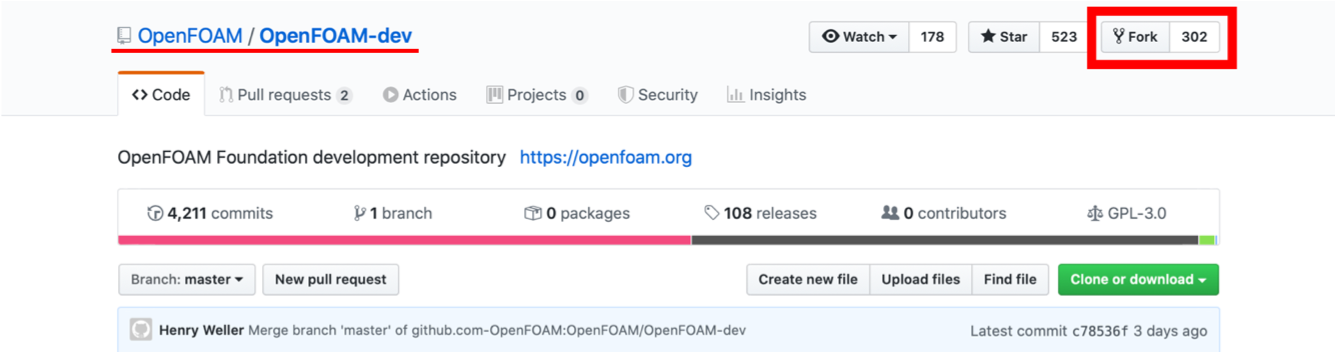
\includegraphics[width=0.8\textwidth]{fig/fig-f1.png}
  \label{fig:f1}
}
%\hspace{0.1\textwidth}
\subfigure[Creating new branch]{
  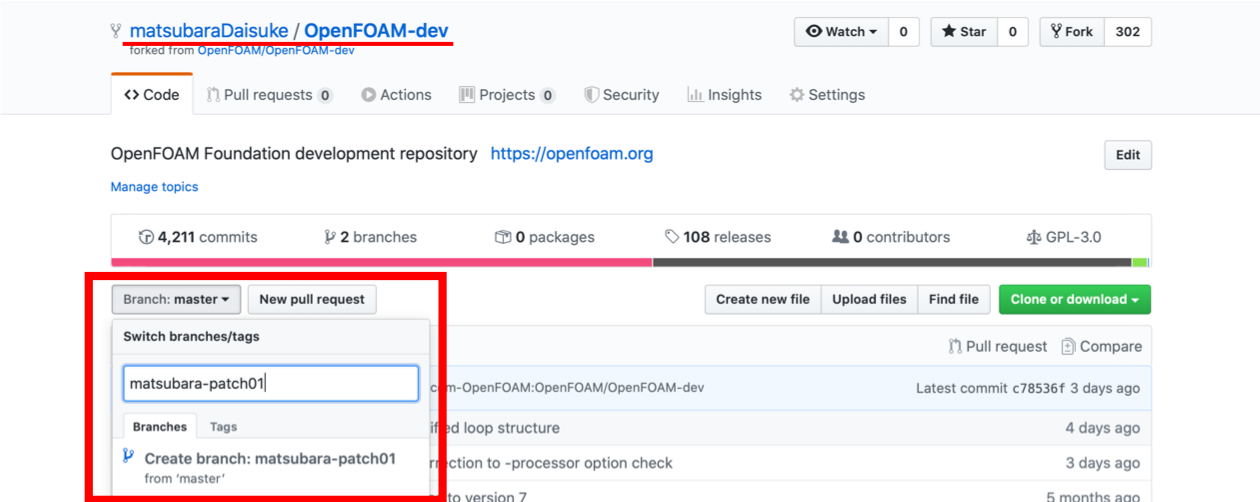
\includegraphics[width=0.8\textwidth]{fig/fig-f2.png}
  \label{fig:f2}
}
\caption{A Explication to fork OpenFOAM-dev repository and to create your new branch.}
\label{fig:f1f2}
\end{figure}
%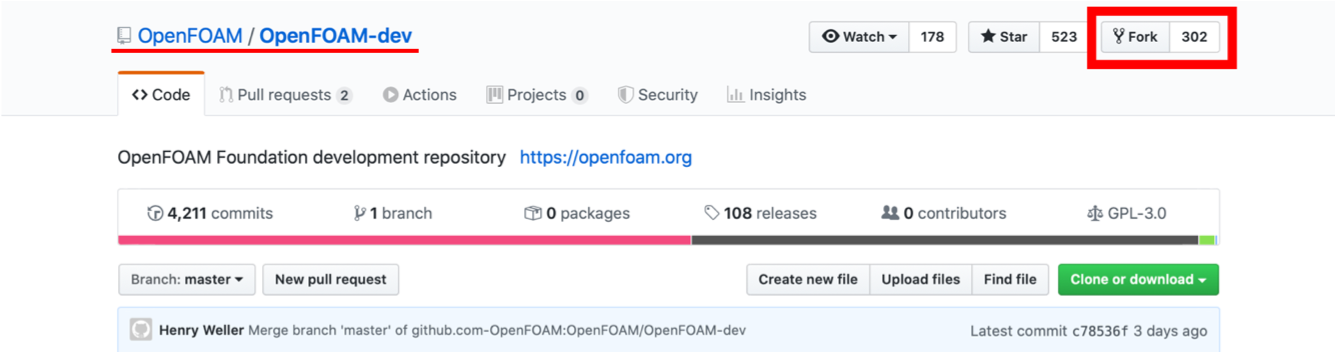
\includegraphics[width=5cm]{fig/fig-f1.png}
%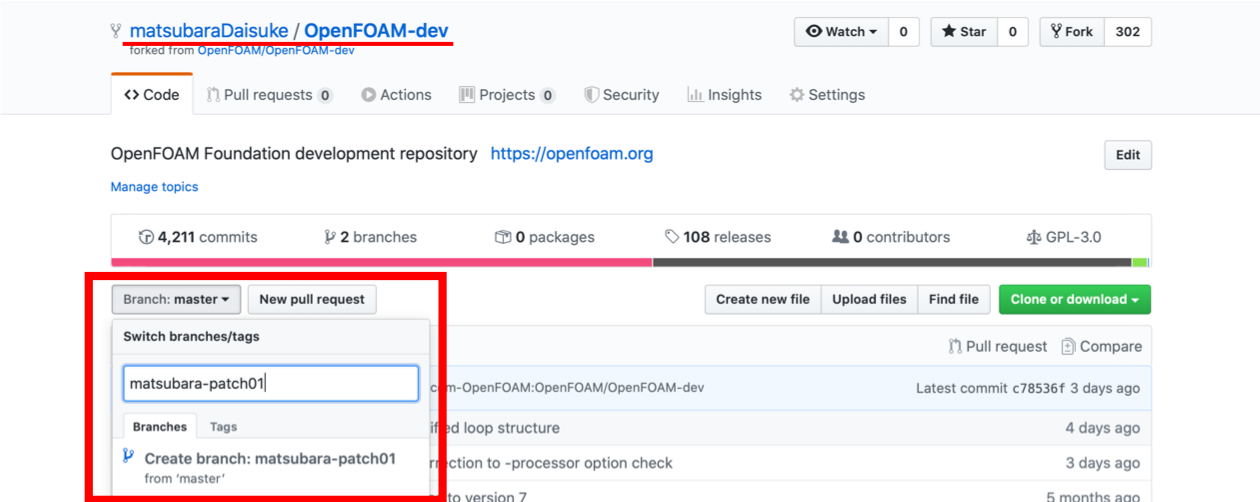
\includegraphics[width=5cm]{fig/fig-f2.png}

次に個人の開発環境に移りターミナル上でgit cloneを行う.(\autoref{fig:f3})例:git clone https://github.com/(githubアカウント名)/OpenFOAM-dev.git
これによって,git cloneしたディレクトリ下にOpenFOAMのプロジェクトがコピーされる.
%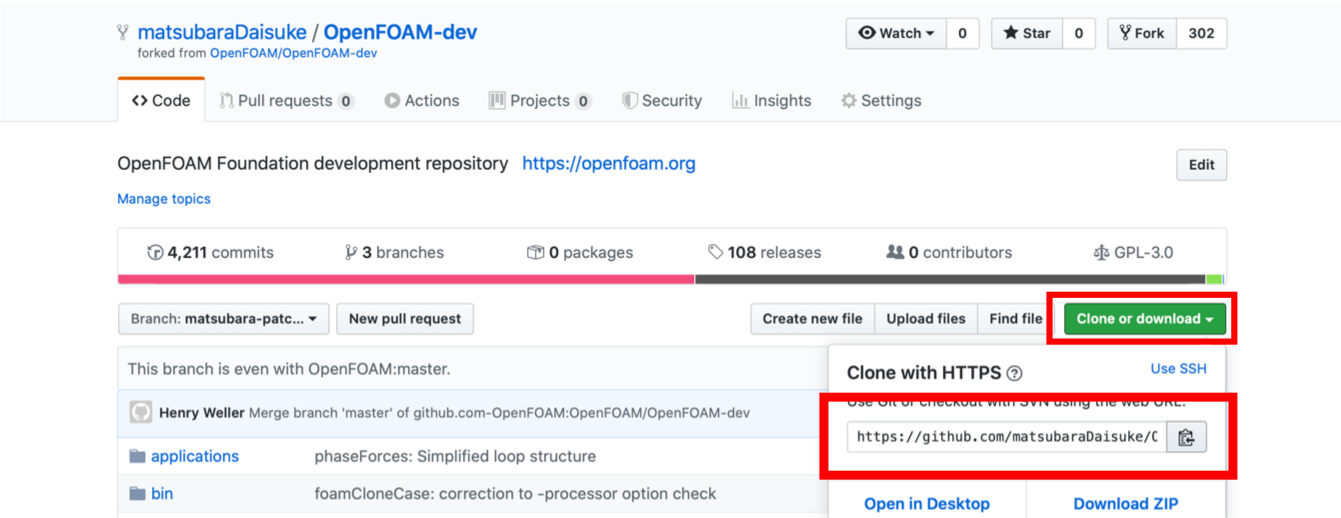
\includegraphics[width=5cm]{fig/fig-f3.png}
\begin{figure}[htbp]
\centering
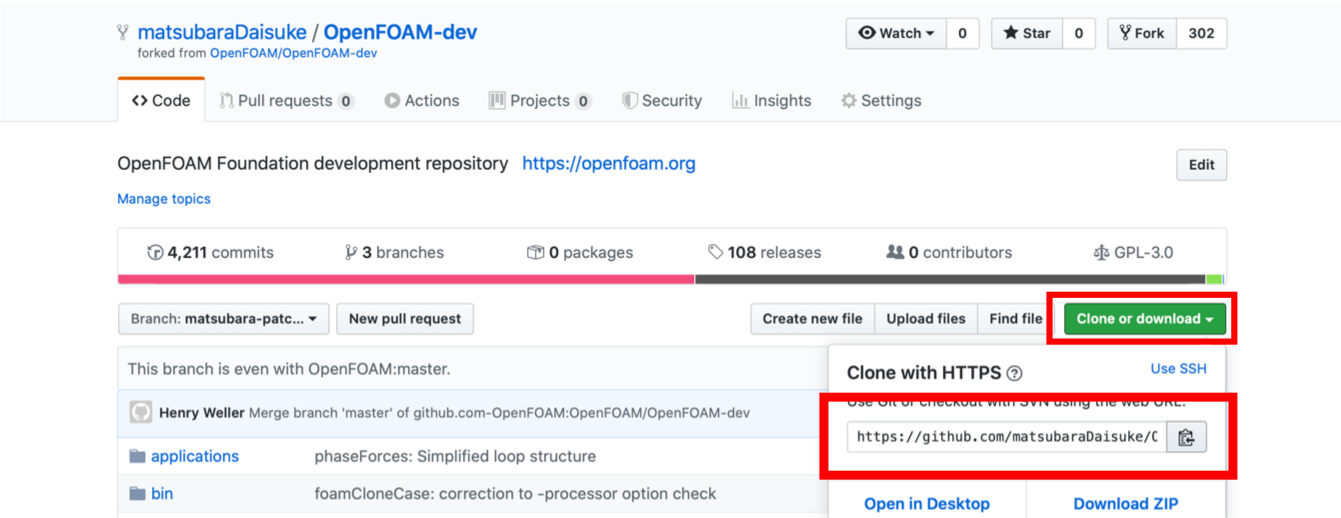
\includegraphics[width=0.8\textwidth]{fig/fig-f3.png}
\caption{Cloning repository on your local machine.}
\label{fig:f3}
\end{figure}

次にgit checkoutにて作成したブランチに切り替える 例:git checkout (開発者名)-patch***
OpenFOAMのプロジェクト内で修正や開発が完了した後,
git add . git commit -m "変更内容のコメント" git push origin (開発者名)-patch***
とすることで,コードの修正内容を個人のgithubのリポジトリに反映させる.
今回の例では以下の様な流れになる.

\begin{shbox}
  \shuser{user}
  \shline{}{git clone https://github.com/matsubaraDaisuke/OpenFOAM-dev.git}  
  \shline{}{cd OpenFOAM-dev}  
  \shline{}{git checkout matsubara-patch1}
\end{shbox}

(コーディング)

\begin{shbox}
  \shuser{user}
  \shline{}{git add .}
  \shline{}{git commit -m "bugfix ******"}
  \shline{}{git push origin matsubara-patch1}
\end{shbox}



最後にgithub上でpull requestを開発元に対して行う.(\autoref{fig:f4})この時コメントに
Fixes issue:
https://bugs.openfoam.org/view.php?id=****
の様に最初に議論したissueのURLを添付するのが慣例のようである.(\autoref{fig:f5})

%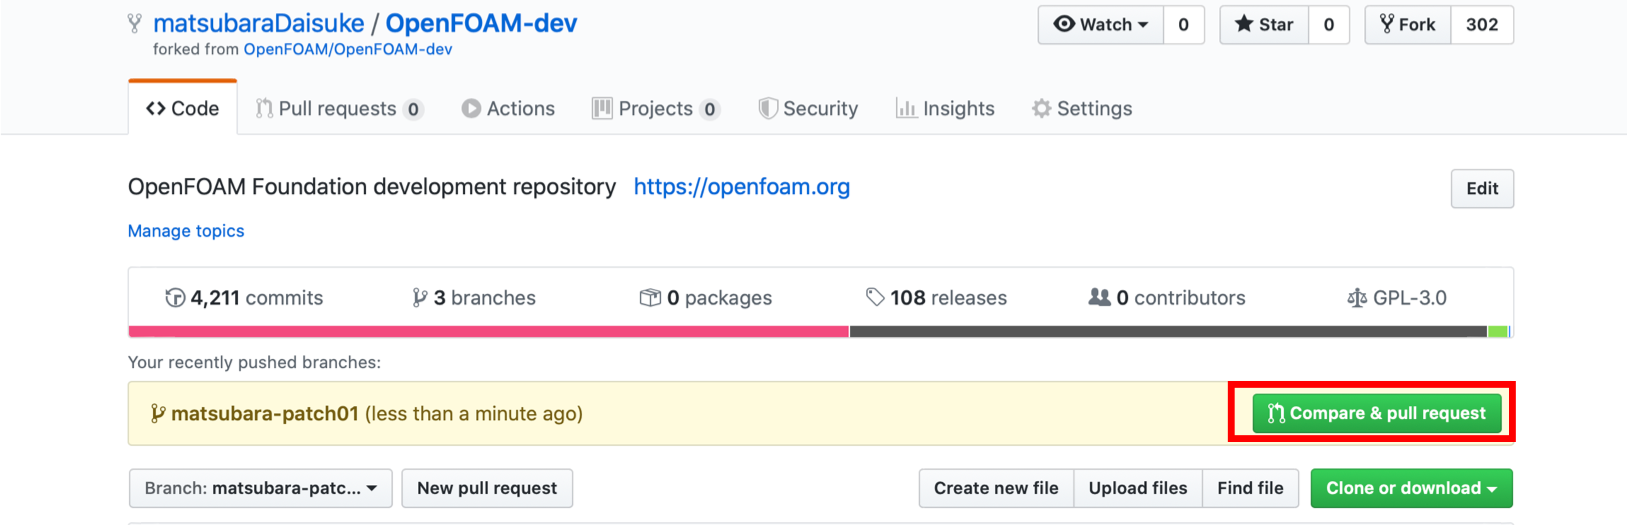
\includegraphics[width=5cm]{fig/fig-f4.png}
%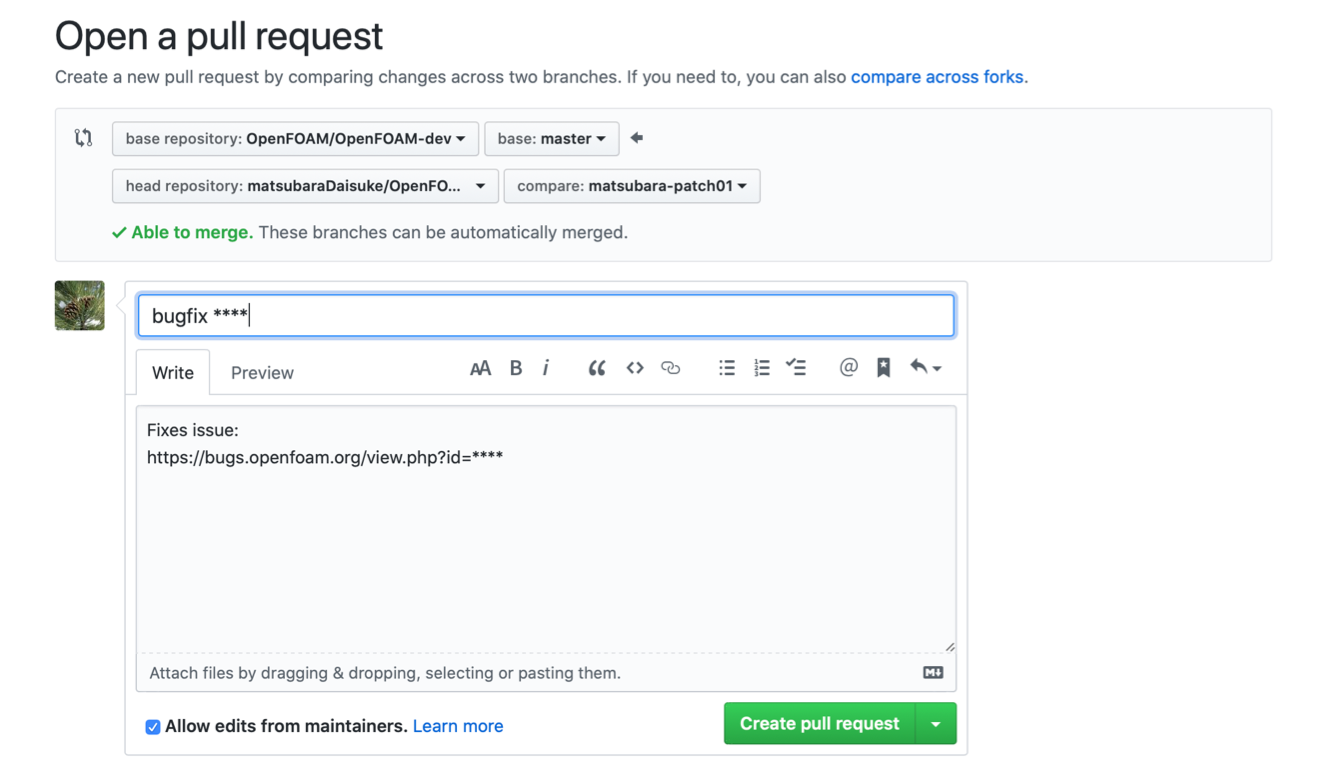
\includegraphics[width=5cm]{fig/fig-f5.png}
\begin{figure}[htbp]
\centering
\subfigure[Pull request your branch into the master branch.]{
  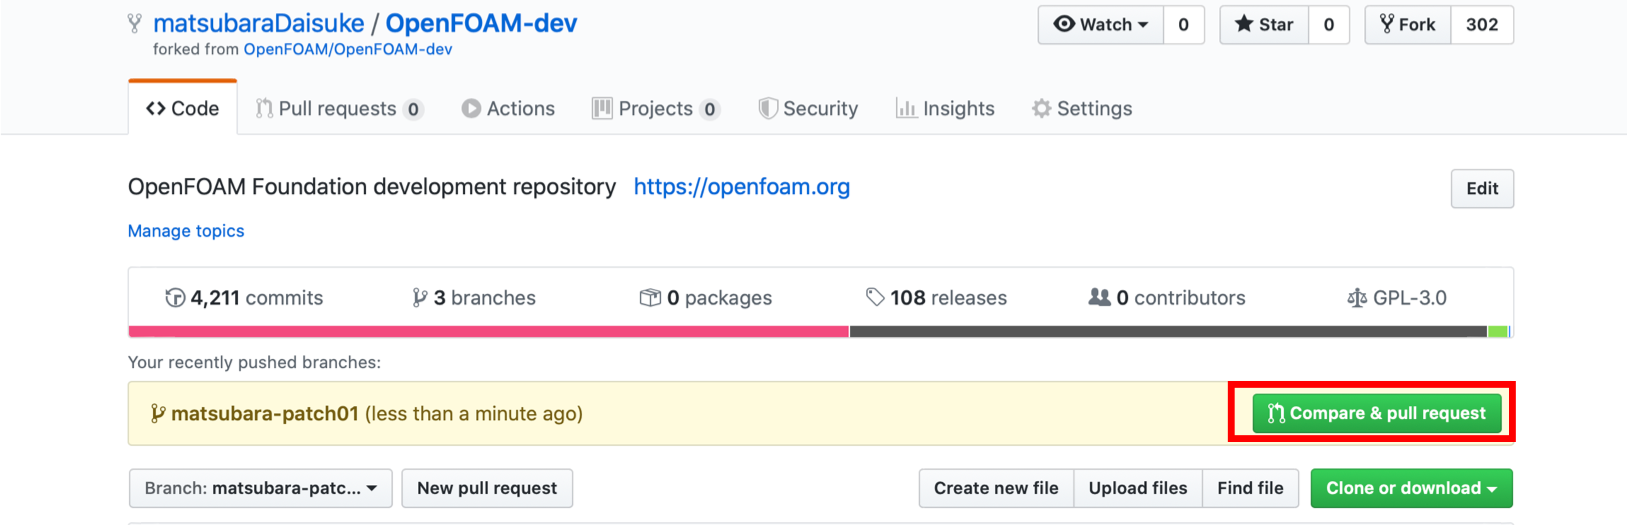
\includegraphics[width=0.8\textwidth]{fig/fig-f4.png}
  \label{fig:f4}
}
%\hspace{0.1\textwidth}
\subfigure[Add your message to pull request.]{
  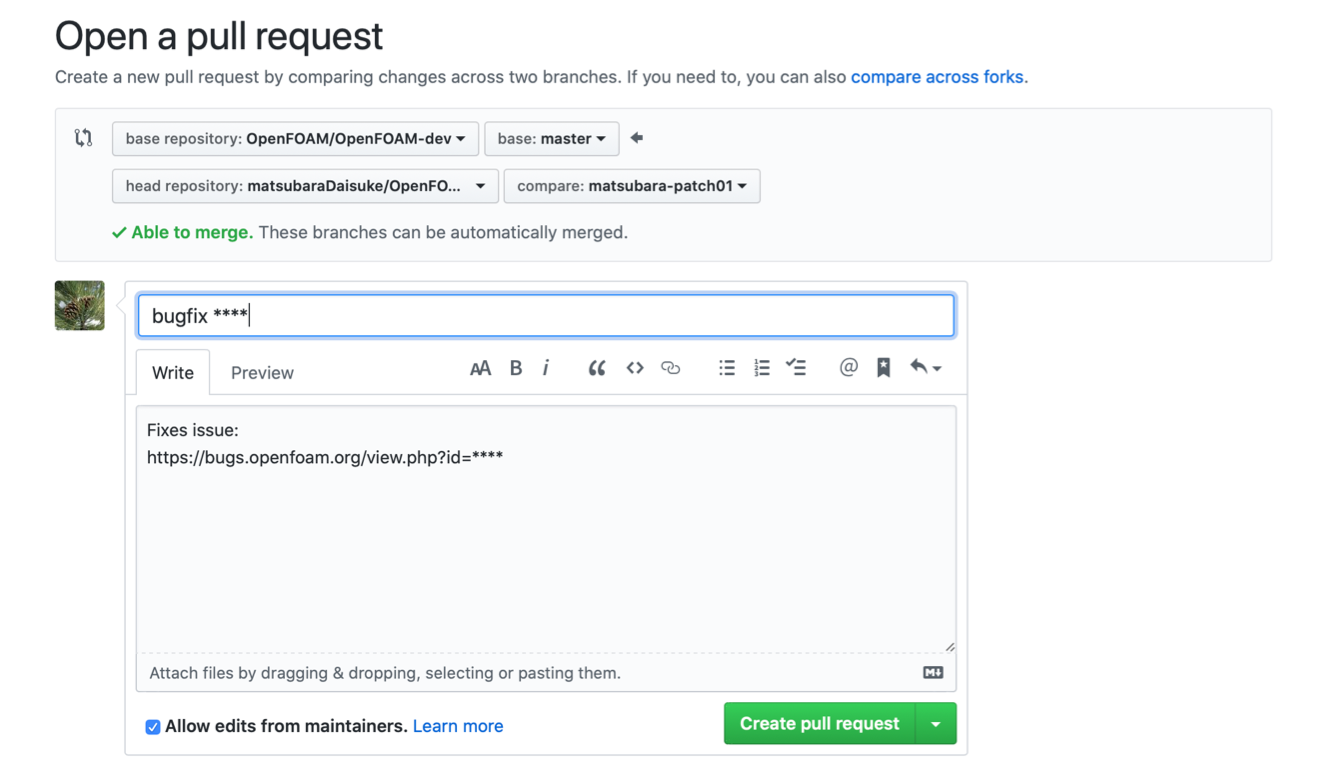
\includegraphics[width=0.8\textwidth]{fig/fig-f5.png}
  \label{fig:f5}
}
\caption{A explication to pull request your branch into the master branch.}
\label{fig:f4f5}
\end{figure}


\section{Gitの使い方}
本節では https://github.com/OpenFOAM-jp/OpenFOAM-jp.git 
のリポジトリにコントリビュートの練習をする方法について解説する.
環境はUbuntu18.04の環境を想定する.
事前に{GitHub}のアカウントを作成する必要がある.
コントリビュートをする際にはまず,Issueを立て自分が加えたい変更について議論する.
Issueを立てる際には以下の内容が含まれていることが望ましい.
\begin{itemize}
  \item 機能の簡単な説明.問題が何であるかの明確で簡潔な説明.
  \item 希望するソリューションの説明.あなたが何をしたいのかについての明確で簡潔な説明.
  \item 検討した代替案を説明.検討した代替ソリューションまたは機能の明確で簡潔な説明.
  \item 追加のコンテキスト.機能リクエストに関する他のコンテキストまたはスクリーンショットをここに追加します.
\end{itemize}
OSSのコントリビュートのバージョン管理ソフトにはGitが一般的に使用されている.
OpenFOAMの開発においてもGitが使用されている.
まずは,Gitをインストールする.

\begin{shbox}
  \shuser{user}
  \shline{}{sudo apt install git}
\end{shbox}

必要なのはソースだけで貢献しないのであれば,次のコマンドでcloneすることで作業は終わる.

\begin{shbox}
  \shuser{user}
  \shline{}{git clone https://github.com/OpenFOAM-jp/OpenFOAM-jp.git}
\end{shbox}

貢献をしたい場合は,OpenFOAM-jpのリポジトリを自分のアカウントにForkする.

TODO: Forkの際の画面キャプチャを挿入する.

Fork後は自分のアカウントのリポジトリをcloneする.

\begin{shbox}
  \shuser{user}
  \shline{}{git clone https://github.com/your\_account\_name/OpenFOAM-jp.git}
\end{shbox}

cloneをしたら自分の環境で実行環境を構築する.
まずは,OpenFOAMを動かすために必要な外部ライブラリをインストールする.

\begin{shbox}
  \shuser{user}
  \shline{}{sudo apt update}
  \shline{}{sudo apt upgrade}
  \shline{}{sudo apt install git-core}
  \shline{}{sudo apt install build-essential}
  \shline{}{sudo apt install cmake}
  \shline{}{sudo apt install libfl-dev}
  \shline{}{sudo apt install bison}
  \shline{}{sudo apt install zlib1g-dev}
  \shline{}{sudo apt install qt4-dev-tools}
  \shline{}{sudo apt install libqt4-dev}
  \shline{}{sudo apt install libqtwebkit-dev}
  \shline{}{sudo apt install gnuplot}
  \shline{}{sudo apt install libreadline-dev}
  \shline{}{sudo apt install libncurses-dev}
  \shline{}{sudo apt install libxt-dev}
  \shline{}{sudo apt install libopenmpi-dev}
  \shline{}{sudo apt install openmpi-bin}
  \shline{}{sudo apt install libboost-system-dev}
  \shline{}{sudo apt install libboost-thread-dev}
  \shline{}{sudo apt install libgmp-dev}
  \shline{}{sudo apt install libmpfr-dev}
  \shline{}{sudo apt install python}
  \shline{}{sudo apt install python-dev}
  \shline{}{sudo apt install libcgal-dev}
  \shline{}{sudo apt install curl}
  \shline{}{sudo apt install git-core}
  \shline{}{sudo apt install build-essential}
  \shline{}{sudo apt install cmake}
  \shline{}{sudo apt install libfl-dev}
  \shline{}{sudo apt install bison}
  \shline{}{sudo apt install zlib1g-dev}
  \shline{}{sudo apt install qt4-dev-tools}
  \shline{}{sudo apt install libqt4-dev}
  \shline{}{sudo apt install libqtwebkit-dev}
  \shline{}{sudo apt install gnuplot}
  \shline{}{sudo apt install libreadline-dev}
  \shline{}{sudo apt install libncurses-dev}
  \shline{}{sudo apt install libxt-dev}
  \shline{}{sudo apt install libopenmpi-dev}
  \shline{}{sudo apt install openmpi-bin}
  \shline{}{sudo apt install libboost-system-dev}
  \shline{}{sudo apt install libboost-thread-dev}
  \shline{}{sudo apt install libgmp-dev}
  \shline{}{sudo apt install libmpfr-dev}
  \shline{}{sudo apt install python}
  \shline{}{sudo apt install python-dev}
  \shline{}{sudo apt install libcgal-dev}
  \shline{}{sudo apt install curl}
\end{shbox}

次に,OpenFOAMのbashrcをターミナル起動時に読み込むように~/.bashrcに登録する.

\begin{shbox}
  \shuser{user}
  \shline{}{echo "source ~/OpenFOAM/OpenFOAM-dev/etc/bashrc" >> ~/.bashrc}
  \shline{}{. ~/.bashrc}
\end{shbox}

ThirdPartyの中のParaViewをインストールする.
この際にpythonを登録するとParaViewのpython拡張機能が使用可能になる.
既にParaViewをインストールしている場合であっても,このParaViewはOpenFOAMの結果表にのプラグインなども同梱しているため,
以下の手順でもう一つインストールすることを推奨する.

\begin{shbox}
  \shuser{user}
  \shline{}{cd \$WM\_THIRD\_PARTY\_DIR}
  \shline{}{./makeParaView -python -python-lib /usr/lib/x86\_64-linux-gnu/libpython2.7.so.1.0}
\end{shbox}

最後にOpenFOAMをインストールする.

\begin{shbox}
  \shuser{user}
  \shline{}{wmRefresh}
  \shline{}{cd \$WM\_PROJECT\_DIR}
  \shline{}{./Allwmake -j | tee log.Allwmake}
\end{shbox}

ソルバーを動かしてインストールの確認を行う.

\begin{shbox}
  \shuser{user}
  \shline{}{mkdir \$WM\_PROJECT\_USER\_DIR}
  \shline{}{cd \$WM\_PROJECT\_USER\_DIR}
  \shline{}{cp -r \$FOAM\_TUTORIALS/basic/potentialFoam/pitzDaily/ ./}
  \shline{}{cd pitzDaily/}
  \shline{}{foamRunTutorials}
  \shline{}{paraFoam}
\end{shbox}

これでParaViewが起動されて結果の表示ができたら完成である.
テストが全てパスしたらソースを変更する.
masterブランチで直接変更することはできないため,ファイルを変更する前に開発ブランチを作成する.

\begin{shbox}
  \shuser{user}
  \shline{}{git branch branch\_name}
\end{shbox}
\begin{shbox}
  \shuser{user}
  \shline{}{git checkout branch\_name}
\end{shbox}

branch\_name には任意の名前を入れる.
自分のアカウント名と加えたい変更について言及されていると分かりやすい.
最初のコマンドでブランチを作成し,2番目のコマンドでブランチに移動する.
これにより,変更を行う準備はほぼ完了である.
変更のラベルを付けるために,連絡先の名前と電子メールを以下のコマンドで指定する.

\begin{shbox}
  \shuser{user}
  \shline{}{git config --global user.name "Your Name Comes Here"}
  \shline{}{git config --global user.email you@yourdomain.example.com}
\end{shbox}

もし src/toto.cc というファイルをいくつか変更したり,新しいファイルとして追加したら,
ローカルのコミットは次のコマンドで行う.
"Your extensive commit message here \#1" には変更に関するメッセージを追加する.
\#1の部分は自分が追加したイシューの番号とする.

\begin{shbox}
  \shuser{user}
  \shline{}{git add src/toto.cc}
  \shline{}{git commit -m "Your extensive commit message here \#1"}
\end{shbox}

この段階ではコミットはあなたのローカルリポジトリで行われていますが,GitHubリポジトリでは行われない.
十分なテストで変更を検証したら,以下のコマンドでGitHubの自分のアカウントのリポジトリに変更を移すことができる.

\begin{shbox}
  \shuser{user}
  \shline{}{git push origin branch\_name}
\end{shbox}

TODO: コマンドのメッセージを含める

このコマンドのメッセージに図のようなURLが表示される.
URLにアクセスしプルリクエストを作成する.

TODO: GetFEMのドキュメントから引用を行っているため言及する.

GetFEM++ のマスターブランチにマージすることは許可されていないので,あなたの役割はここで終わる.
プルリクエストのページで管理者や他の開発者と議論することができる.
管理者が承認した場合には変更がマージされる.

いくつかの便利なgitコマンドを示す.

\begin{shbox}
  \shuser{user}
  \shline{}{git status  : status of your repository / branch}
  \shline{}{git log --follow "filepath"   : Show all the commits modifying the specified file (and follow the eventual change of name of the file).}
  \shline{}{gitk --follow filename : same as previous but with a graphical interface}
\end{shbox}

\section{GitHub および Travis による継続的インテグレーション}
Travis CIは,GitHub上のソフトウェアのビルドやテストを行う,オンラインで分散型の継続的インテグレーション (CI) サービスである.
継続的インテグレーションサービスとは,ビルドやテストを継続的に自動実行するサービスである.
継続的インテグレーションを行うことにより,機能追加やリファクタリングによるデグレードを防ぐことができる.
以下に,GetFEM++で使用している.travis.ymlを示す.
リポジトリにymlファイルを追加することで,Travisによるインテグレーションテストが実行される.
今後OpenFOAMのリポジトリでもCIが実行できるようにする予定である.
\begin{lstlisting}
language: python
python:
  - "3.6"
sudo: false
dist: bionic
cache:
  directories:
  - $HOME/.cache/pip
before_install:
- sudo apt-get install -y --no-install-recommends automake
- sudo apt-get install -y --no-install-recommends libtool
- sudo apt-get install -y --no-install-recommends make
- sudo apt-get install -y --no-install-recommends g++
- sudo apt-get install -y --no-install-recommends libqd-dev
- sudo apt-get install -y --no-install-recommends libqhull-dev
- sudo apt-get install -y --no-install-recommends libmumps-seq-dev
- sudo apt-get install -y --no-install-recommends liblapack-dev
- sudo apt-get install -y --no-install-recommends libopenblas-dev
- sudo apt-get install -y --no-install-recommends libpython3-dev
- sudo apt-get install -y --no-install-recommends ufraw
- sudo apt-get install -y --no-install-recommends imagemagick
- sudo apt-get install -y --no-install-recommends fig2dev
- sudo apt-get install -y --no-install-recommends texlive
- sudo apt-get install -y --no-install-recommends xzdec
- sudo apt-get install -y --no-install-recommends fig2ps
- sudo apt-get install -y --no-install-recommends gv
- pip install -r requirements.txt
addons:
  apt:
    update: true
script:
- bash autogen.sh
- export CXXFLAGS=-coverage
- export LDFLAGS=-coverage
- export CPPFLAGS=-coverage
- export CFLAGS=-coverage
- export FCFLAGS=-coverage
- ./configure --with-pic
- make -j8
- make -j8 check
- (cd doc/sphinx; make html)
after_success:
- bash <(curl -s https://codecov.io/bash)
\end{lstlisting}

TODO Travis CIについてWikipediaからの引用であることを明記する.

TODO 継続的インテグレーションサービスについてWikipediaからの引用であることを明記する.
%
\section{OpeFOAM-jp}
OpenFOAM-jp\cite{URL:OpenFOAM-jp}は今回立ち上がったコミュニティの活動を行うためのGiuHubレポジトリである.
目的は日本のOpenFOAMコミュニティの活性化,OpenFOAMへのコントリビュートの入り口,およびOSSコントリビュート活動の学習の場としている.
参加は誰でも国籍を問わず可能であり,今後人口が増えてオープンで有意義な場として機能することを期待する.
%
\subsection{OpenFOAM-jp/issues}
issuesレポジトリ\cite{URL:OpenFOAM-jp-issues}は最初の議論を行う場として設置された.
テキストエディタVimの日本コミュニティのレポジトリ\cite{URL:vim-jp}のForkであり,運用方法もこれを参考にする.
ここではOpenFOAMの新機能の提案やOpenFOAM-jpで行う活動の議論などを行うことを目的としている.
質問掲示板であるGoogle Forumと役割が重複すると混乱や情報の偏りを発生させるため明確な差別化を行うように注意して運用していく.
%
\subsection{OpenFOAM-jp/OpenFOAM-jp}
OpenFOAM-jpレポジトリ\cite{URL:OpenFOAM-jp-OpenFOAM-jp}はFoundation版のOpenFOAM-devのForkであり,pushやPull Requestなどのgitの基本機能の練習用に設置された.
branchを作成してオリジナルの機能を配布する目的で使用することも期待している.
エラーメッセージの日本語化プロジェクトなども予定している.
%
\subsection{OpenFOAM-jp/OpenFOAM-utilities-tutorials-jp}
OpenFOAM-utilities-tutorials-jp\cite{URL:OpenFOAM-jp-OpenFOAM-utilities-tutorials-jp}は,web上にあまり情報のないOpenFOAMのutilitiesに関するまとめを行う目的で設置された.
その一例を\autoref{fig:utilities-example}に示す.
\begin{figure}[htbp]
\centering
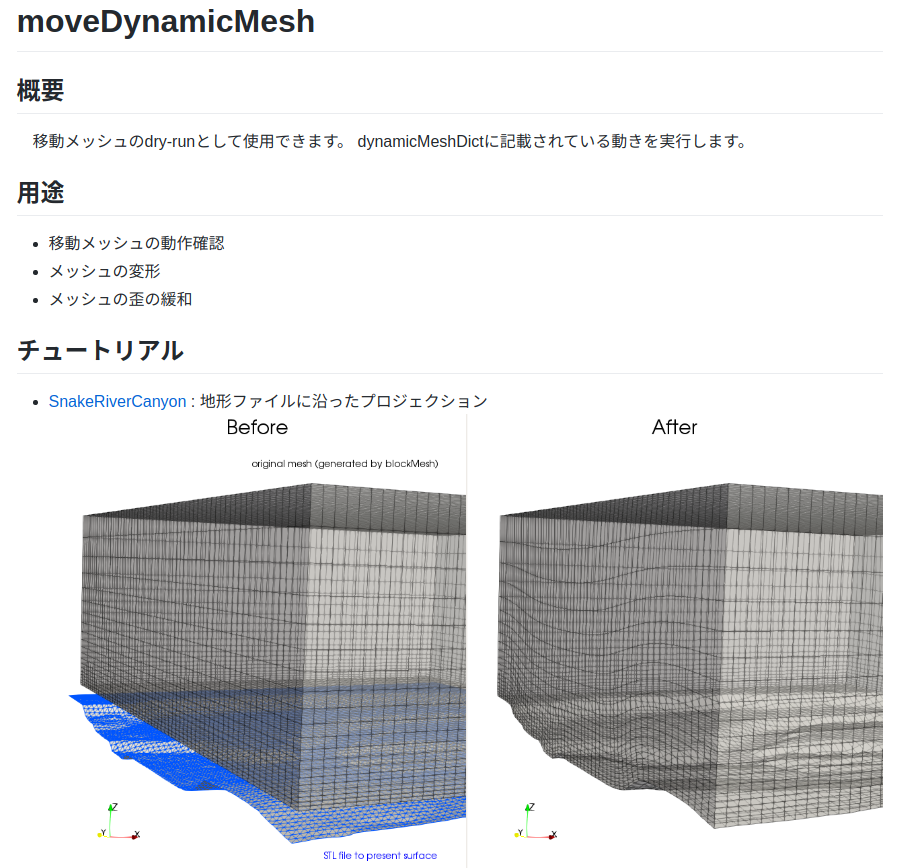
\includegraphics[width=0.8\textwidth]{fig/utilities-example.png}
\caption{moveDynamicMesh(v1906) utilitiy's tutorial document.\cite{URL:OpenFOAM-jp-movedDynamicMesh}}
\label{fig:utilities-example}
\end{figure}
各utilityについて,使用方法をMarkDown形式のドキュメントでまとめ,そのチュートリアルを作成する.
ディレクトリ構成は実際のソースコードに準拠し,最表層のMarkDownファイルから各ドキュメントにアクセスできるようにしている.\cite{URL:OpenFOAM-jp-util-index}
現時点ではOpenFOAM-v1906について作成中である.
%
\section{まとめ}

%%%
%%% OpenCAEシンポジウムTeXテンプレートファイル
%%% OpenFAOM-jp_OpenCAE_symposium.tex
%%% OpenCAEシンポジウム2018版
%%%
%%
%% ltjocはOpenCAE論文集・シンポジウム用のクラスファイルです.変更しないでください.
%% 本文が英語の場合には,オプションにenglishを指定してください.
\documentclass{ltjoc}
%\documentclass[english]{ltjoc}
\usepackage[
 backgroundcolor=gray!50,
 usernamecolor=black,
 machinenamecolor=black,
 indicatorcolor=black,
 separatorcolor=black,
 pathcolor=black,
 optioncolor=black,
 textcolor=black
]{shdoc}
%%
%% 表題(title),副題(subtitle),著者(author),所属(affiliation)
%% 本文が英語の場合には,こちらに英文表題,英文副題,英文著者,英文所属を記述します.
\title{OpenFOAMコントリビュート活動}
% 副題が無い場合にはコメントアウトします.
% \subtitle{\TeX のテンプレート(和文副題)} 
\author{%
稲葉竜一$^{1\dagger}$%
\hspace{1\zw}%
松原 大輔$^{2}$%
\hspace{1\zw}%
@tkoyama010$^{1}$%
}
\affiliation{%
${}^{1}$OpenFOAM-jp%
\hspace{1\zw}%
${}^{2}$オープン CAE勉強会%
} 
%%
%% Corresponding authorの電子メールアドレス
%% 本論文について連絡が取れる著者の電子メールアドレスを記載してください.
\AuthorsEmail{inabower@gmail.co.jp}
%%
%% 英文表題(etitle),英文副題(esubtitle),英文著者(eauthor),英文所属(eaffiliation)
%% 本文が英語の場合には表示されません.
\etitle{OpenFOAM Contributing Activities}
% 副題が無い場合にはコメントアウトします.
% \esubtitle{The case of \TeX (English Sub-Title)}
\eauthor{%
Ryuichi INABA$^{*\dagger}$%
\hspace{1em}%
Daisuke MATSUBARA$^{**}$%
\hspace{1em}%
@tkoyama010$^{*}$%
}
\eaffiliation{%
${}^{*}$OpenFOAM-jp%
\hspace{1em}%
${}^{**}$OpenCAE Local user group%
}
%%
%% キーワード
\keywords{GitHub, git, Pull Request, OpenFOAM, develop}
%%
%% 英文概要
%% 英文概要を省略する場合には,abstract環境の定義をしないでください.
\begin{abstract}
Commits from Japanese to OpenFOAM are less.
So, we established a group called OpenFOAM-jp by volunteers.
We started contributing activities such as development of software,
translation of documents and preparation of tutorials.
We will report how to join our activity by using git and GitHub.
\end{abstract}
%%
%% luatexja-fontspecパッケージ
\usepackage{luatexja-fontspec}
\defaultfontfeatures{Ligatures=TeX}
%% luatexja-presetパッケージ
%% 和文フォントのプリセット設定
%% オプションにnoembed(非埋込)を指定しないでください.
%\usepackage[ipaex]{luatexja-preset} % IPAex(デフォルト)
%\usepackage[ms]{luatexja-preset} % MS
%\usepackage[hiragino-pro]{luatexja-preset} % ヒラギノPro
%%
%% 欧文フォントの指定
%% 使用できるフォントについては,以下のコマンドで調べてください.
%% $ luaotfload-tool --list=*
%%
%% 欧文通常フォント
%\setmainfont{Cambria} % Cambria
%\setmainfont{Times New Roman} % Times New Roman
%\setmainfont{TeXGyreTermes} % TeXGyreTermes
%%
%% 欧文Sans-serifフォント
%\setsansfont{Calibri} % Calibri
%\setsansfont{Arial} % Arial
%\setsansfont{Helvetica} % Helvetica
%\setsansfont{TeXGyreHeros} % TeXGyreHeros
%%
%% 欧文monospaceフォント
%\setmonofont{Consolas} % Consolas
%\setmonofont{Courier New} % Courier New
%\setmonofont{Lucida Console} % Lucida Console
%%
%% subfigureパッケージ
\usepackage{subfigure}
%%
%% graphicxパッケージ
\usepackage{graphicx}
%%
%% hyperrefパッケージ
\usepackage[
 pdfencoding=auto,
 bookmarks=true,
 bookmarksnumbered=true,
 colorlinks=true,
 allcolors={blue}
]{hyperref}
%%
%% listingsパッケージ
\usepackage{listings}
\renewcommand{\lstlistingname}{Code}
\lstset{
basicstyle={\footnotesize\ttfamily},
commentstyle=\color{blue},
frame={tb},
breaklines=true,
columns=[l]{fullflexible},
numbers=left,
numberstyle={\footnotesize},
keepspaces=true
}
%%
%% autorefでの図表の参照名の再定義
\makeatletter
\if@english
  \renewcommand*{\figureautorefname}{\figurename}
  \renewcommand*{\tableautorefname}{\tablename}
\else
  \renewcommand*{\figureautorefname}{図}
  \renewcommand*{\tableautorefname}{表}
\fi
\makeatother
%%
%% ヘッダ右の設定
%% 変更しないでください.
\markright{Open CAE Symposium 2019, Dec. 19-21, 2019, Osaka, D-2} % Do not edit this line
%%
%% 本文
\begin{document}
%%
%% 題目などの出力
\maketitle
%%%
\section{はじめに}
現状日本からのOpenFOAMへのコントリビュートは少ない.
そこで有志により"OpenFOAM-jp"といグループを立ち上げ,本家の開発やドキュメントの翻訳,チュートリアルの作成などのコントリビュート活動を始めた.
本報告ではその活動内容などについて発表する.
\section{Foundation版とESI版の違い}
OpenFOAMは,Imperial Collageで開発された商用CFDコードFOAM(Field Operation And Manipulation)が,2004年にOpenFOAMと名前を変えてオープンソースとしてリリースされたことから始まる.\cite{URL:openfoam.history}\cite{Minabe:OpenCAE2015-GP23}
2011年にはOpenFOAMを運営しているOpenCFD社がSGI社に買収され,またその2社によりOpenFOAMの商標を譲渡したOpenFOAM Foundation Inc.を設立した.
これ以降OpenFOAMはOpenFOAM Foundation Inc.より開発と配布が行われており,2019年11月現在OpenFOAM-V7を最新版とするForkが”Foundation版”\cite{URL:openfoam.org}\cite{URL:GitHub-foundation}と呼ばれている.

一方でOpenFOAMには多くのForkが存在する.
2012年以降はESI社がOpenCFD社の買収という形から開発に加わるようになり,
2016年にはOpenFOAM-v3.0からForkしたOpenFOAM-v3.0+をリリースした.
2019年11月時点ではこの最新版はOpenFOAM-v1906であり,このForkが”ESI版”\cite{URL:openfoam.com}\cite{URL:GitLab-plus}もしくは”plus版”と呼ばれる.

本報告ではこのFoudation版とESI版の2つについてコントリビュートの流れなどを報告する.
%
\section{ESI版コントリビュート方法}
ESI版の開発はGitLabで行われている.\cite{URL:GitLab-plus}
このページからレポジトリをcloneすることができ,これをそのままコンパイルすることで次期リリース予定のESI版OpenFOAMを使用することができる.
またここには開発途中のbranchが多くあり,将来的に追加されるであろう機能をチェックすることもできる.

\autoref{fig:plus-register}に示すGitLabのページの右上のボタンからこのOpenFOAM-plusのレポジトリに登録することもでき,これによりissueの作成や書き込みをすることができるようになる.
\begin{figure}[htbp]
\centering
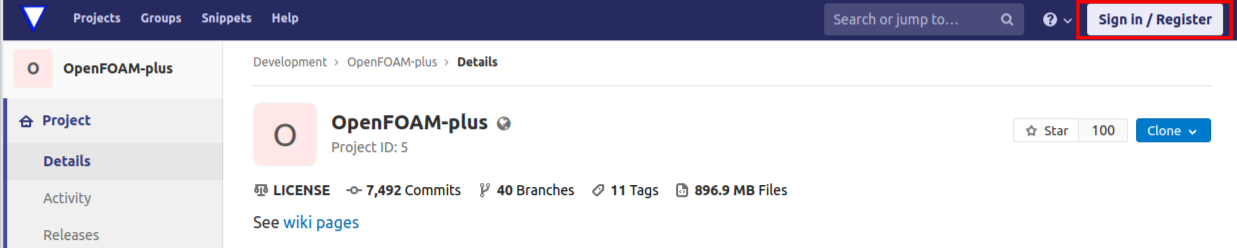
\includegraphics[width=0.8\textwidth]{fig/plus_register.png}
\caption{A register button of OpenFOAM-plus's GitLab page.}
\label{fig:plus-register}
\end{figure}
例えばバグを見つけた場合やOpenFOAMへの要望がある場合には,issueを作成することで開発者へ周知することができ,必要と判断された場合には開発者によりコードの修正や作成が行われる.
\autoref{fig:plus-issue}には実際に作成したissueの例を示す.内容としてはソルバーのDiscriptionの中のスペルミスを指摘した簡単なものであるが,数日以内に@mark氏により該当箇所の修正が行われていることが確認できる.
\begin{figure}[htbp]
\centering
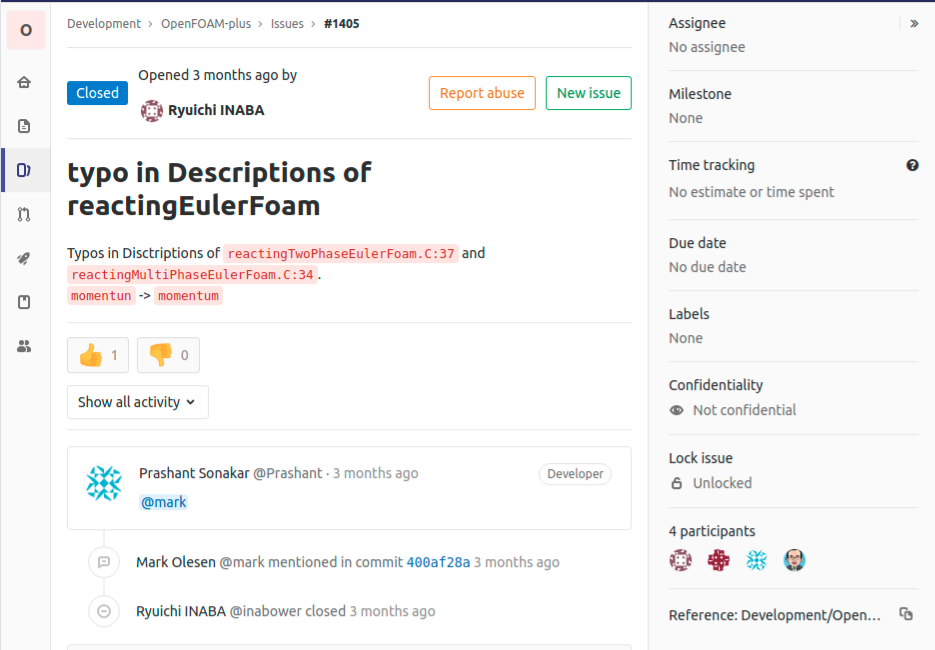
\includegraphics[width=0.8\textwidth]{fig/plus_issue.png}
\caption{An Example issue to fix typo.}
\label{fig:plus-issue}
\end{figure}
このような小さなコントリビュートの積み重ねがOSSであるOpenFOAMを精錬していくこととなる.

一方で,pushやPull Requestなどのコードの変更を行うための権限は制限されている.
このため,ESI版OpenFOAMのコードにコントリビュートする手段としては,開発メンバーに加わらない限りはissueの作成もしくはissue内の議論へ参加することに限られる.
なお2019年11月現在OpenFOAM-plusの開発メンバーは15名であり,実力や面識,貢献頻度が担保されたメンバーで開発を行っていることが推察される.\cite{URL:GitLab-plus-members}
%
\section{Foundation版コントリビュート方法}

Foundation版の開発はGithubで行われている.Foundation版ではissueの管理はGithubでは行わないので注意が必要である.バグ報告は専用のissueTrackingのページへ登録する必要がある.
未登録の場合は,名前とメールアドレスを入力し,返信のリンクを辿ることでviewerとして参加することができる.
また数時間後にスパムでないことが認められると,reporterに昇格できる.
reporterとなることでissueを立てて,バグの報告が可能となる.
ここでバグの重要度や改善方法を議論をすることになる.
issueTrackingの内容を確認すると,Foundation版は基本的にbugfixを目的としたコントリビュートが主の様である.

重大なバグの修正または,新しい開発を提供する場合,OpenFOAM Foundation Contributor Agreementに署名する必要がある.
Foundation版HPのメニューバーのDevelopment/ContributorAgreeementのリンクを辿り,Contact Usのページから名前と所属,コントリビュートに参加した意思を記載して送信すると,後日,Henry G. WellerからPDF形式の登録用紙が送付されてくる.
登録用紙の内容は,前述のContributorAgreeementのページに記載されているものと同じである.

バグの修正などでFoundation版のOpenFOAMの修正を開発元に共有する場合,Foundation版のOpenFOAMはgithub上で管理されているため,githubアカウントが必要となる.

コントリビュートで最初に行うことは開発元のリポジトリをForkすることから始まる.(\autoref{fig:f1})
Forkしたことにより,自身のgithubアカウントにOpenFOAMのリポジトリが作成されていることが確認できる.
次に開発用の新しいブランチを作成する.ブランチ名は「(開発者名)-patch***」などとするとよいだろう.今回の例では「matsubara-patch1」とした.(\autoref{fig:f2})

\begin{figure}[htbp]
\centering
\subfigure[A fork button of Github page]{
  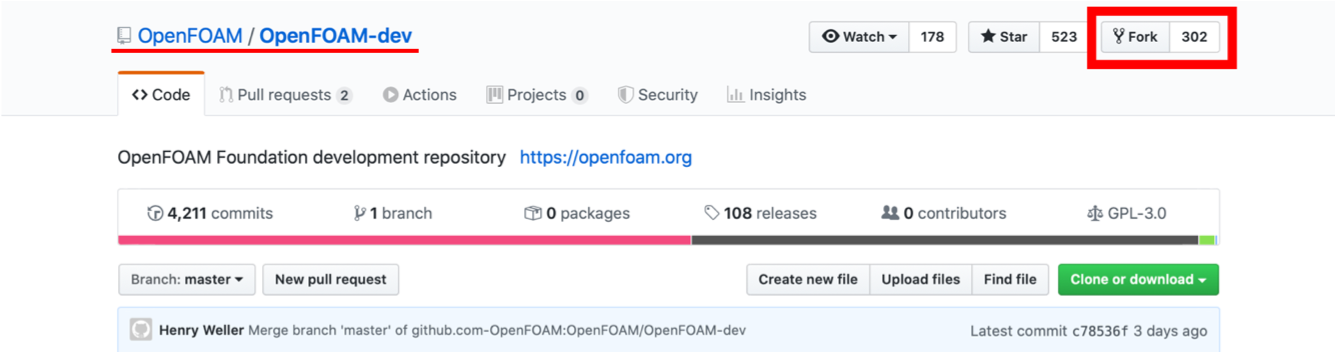
\includegraphics[width=0.8\textwidth]{fig/fig-f1.png}
  \label{fig:f1}
}
%\hspace{0.1\textwidth}
\subfigure[Creating new branch]{
  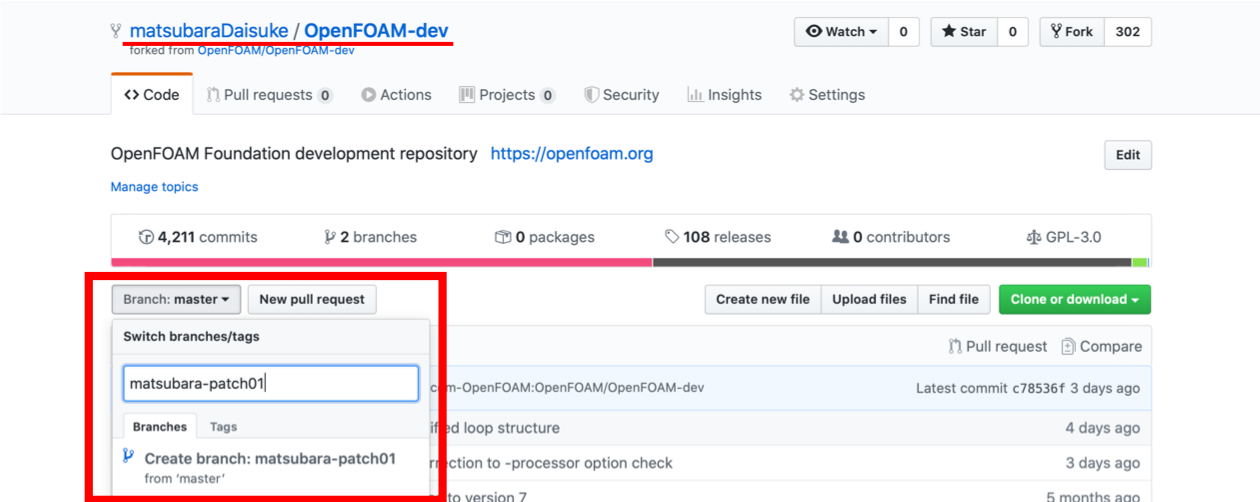
\includegraphics[width=0.8\textwidth]{fig/fig-f2.png}
  \label{fig:f2}
}
\caption{A Explication to fork OpenFOAM-dev repository and to create your new branch.}
\label{fig:f1f2}
\end{figure}
%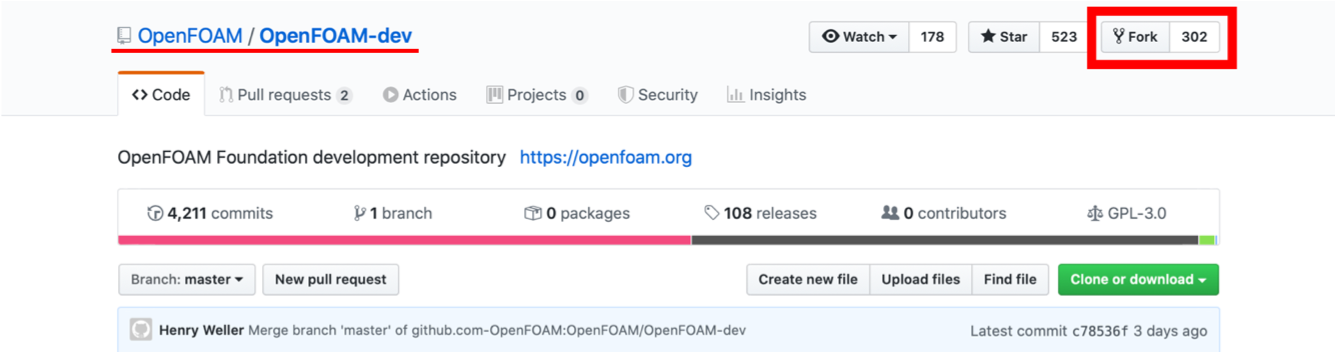
\includegraphics[width=5cm]{fig/fig-f1.png}
%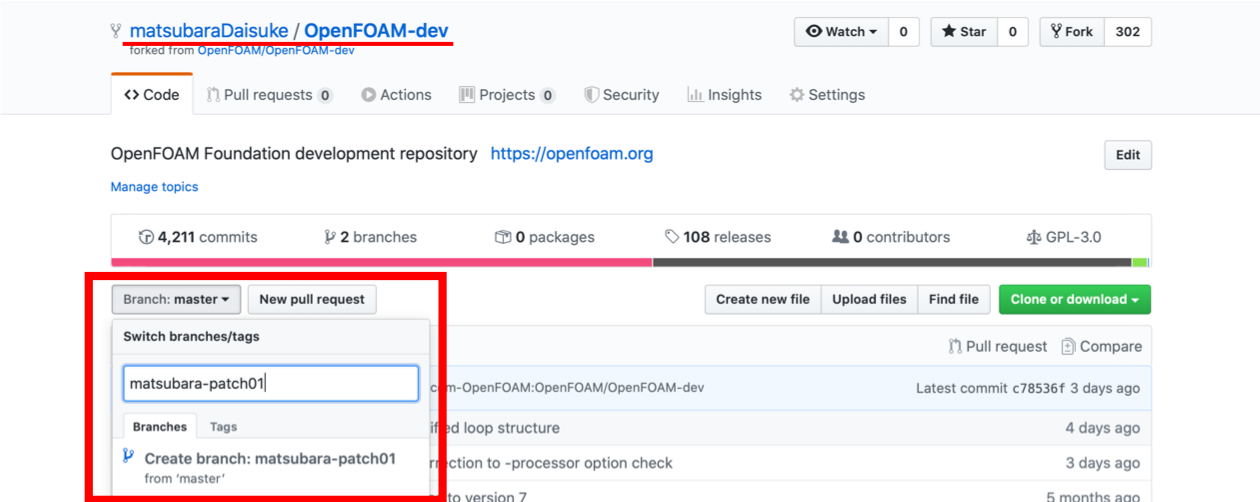
\includegraphics[width=5cm]{fig/fig-f2.png}

次に個人の開発環境に移りターミナル上でgit cloneを行う.(\autoref{fig:f3})例:git clone https://github.com/(githubアカウント名)/OpenFOAM-dev.git
これによって,git cloneしたディレクトリ下にOpenFOAMのプロジェクトがコピーされる.
%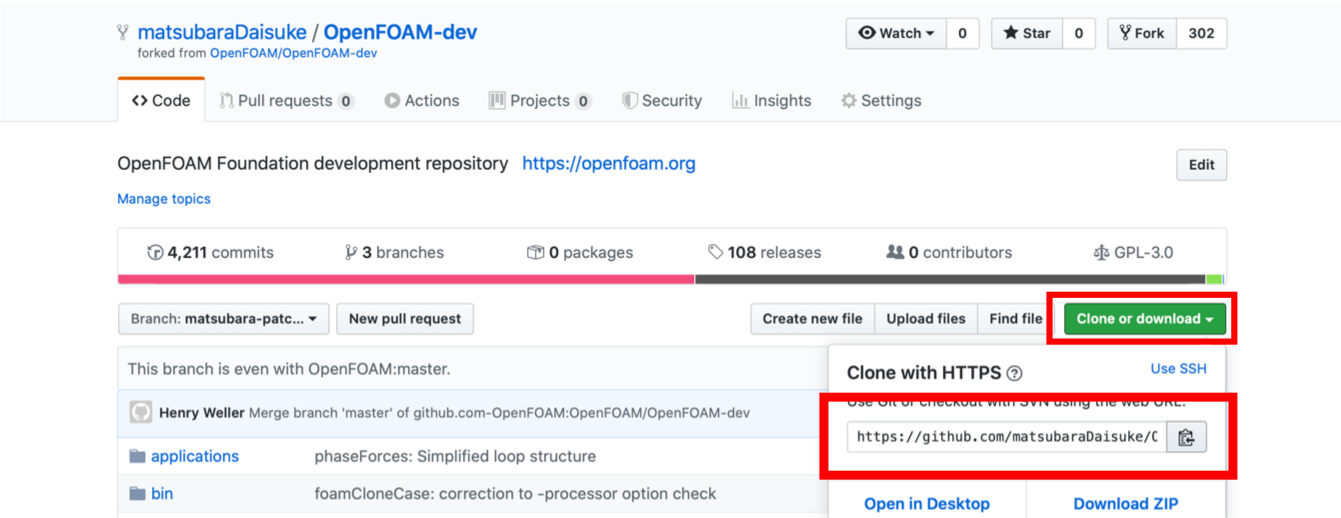
\includegraphics[width=5cm]{fig/fig-f3.png}
\begin{figure}[htbp]
\centering
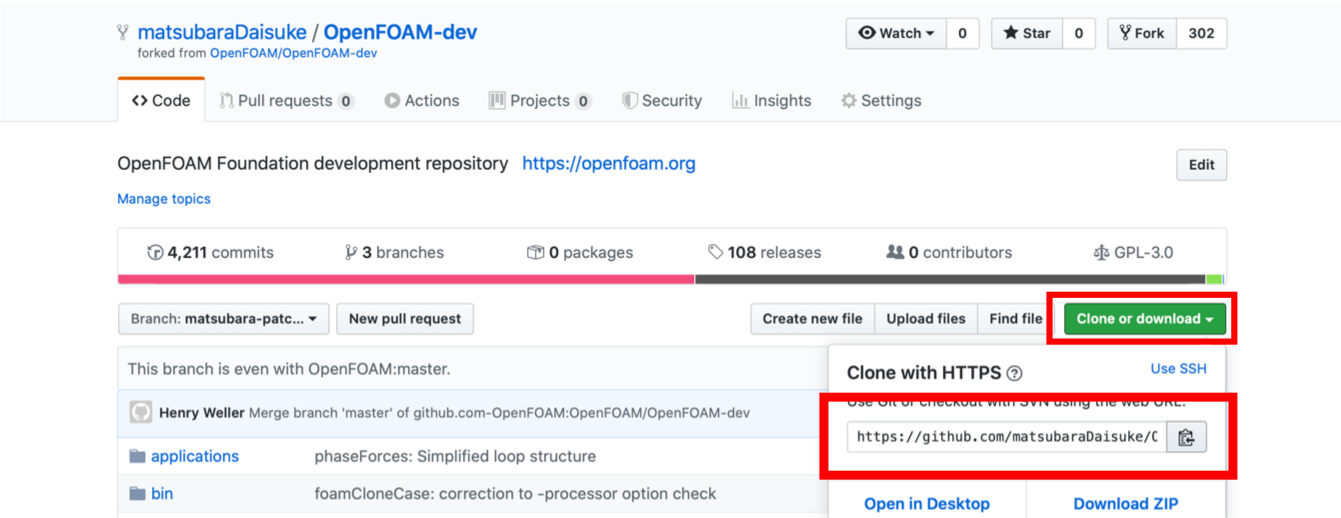
\includegraphics[width=0.8\textwidth]{fig/fig-f3.png}
\caption{Cloning repository on your local machine.}
\label{fig:f3}
\end{figure}

次にgit checkoutにて作成したブランチに切り替える 例:git checkout (開発者名)-patch***
OpenFOAMのプロジェクト内で修正や開発が完了した後,
git add . git commit -m "変更内容のコメント" git push origin (開発者名)-patch***
とすることで,コードの修正内容を個人のgithubのリポジトリに反映させる.
今回の例では以下の様な流れになる.

\begin{shbox}
  \shuser{user}
  \shline{}{git clone https://github.com/matsubaraDaisuke/OpenFOAM-dev.git}  
  \shline{}{cd OpenFOAM-dev}  
  \shline{}{git checkout matsubara-patch1}
\end{shbox}

(コーディング)

\begin{shbox}
  \shuser{user}
  \shline{}{git add .}
  \shline{}{git commit -m "bugfix ******"}
  \shline{}{git push origin matsubara-patch1}
\end{shbox}



最後にgithub上でpull requestを開発元に対して行う.(\autoref{fig:f4})この時コメントに
Fixes issue:
https://bugs.openfoam.org/view.php?id=****
の様に最初に議論したissueのURLを添付するのが慣例のようである.(\autoref{fig:f5})

%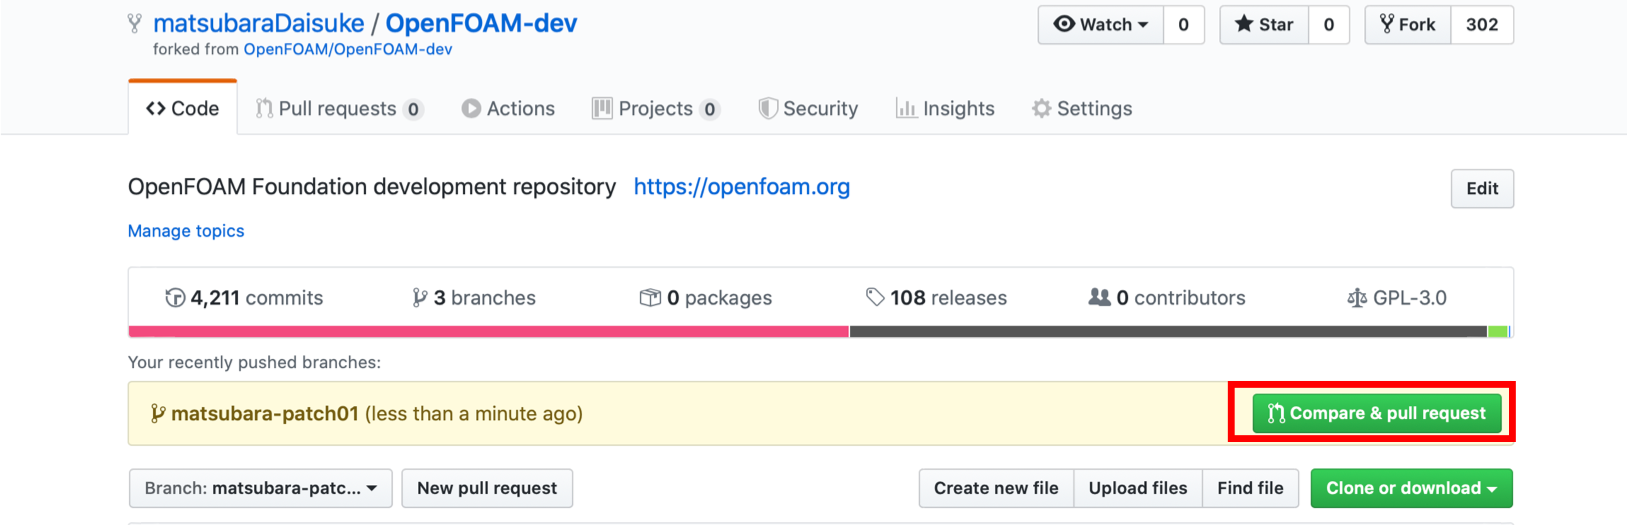
\includegraphics[width=5cm]{fig/fig-f4.png}
%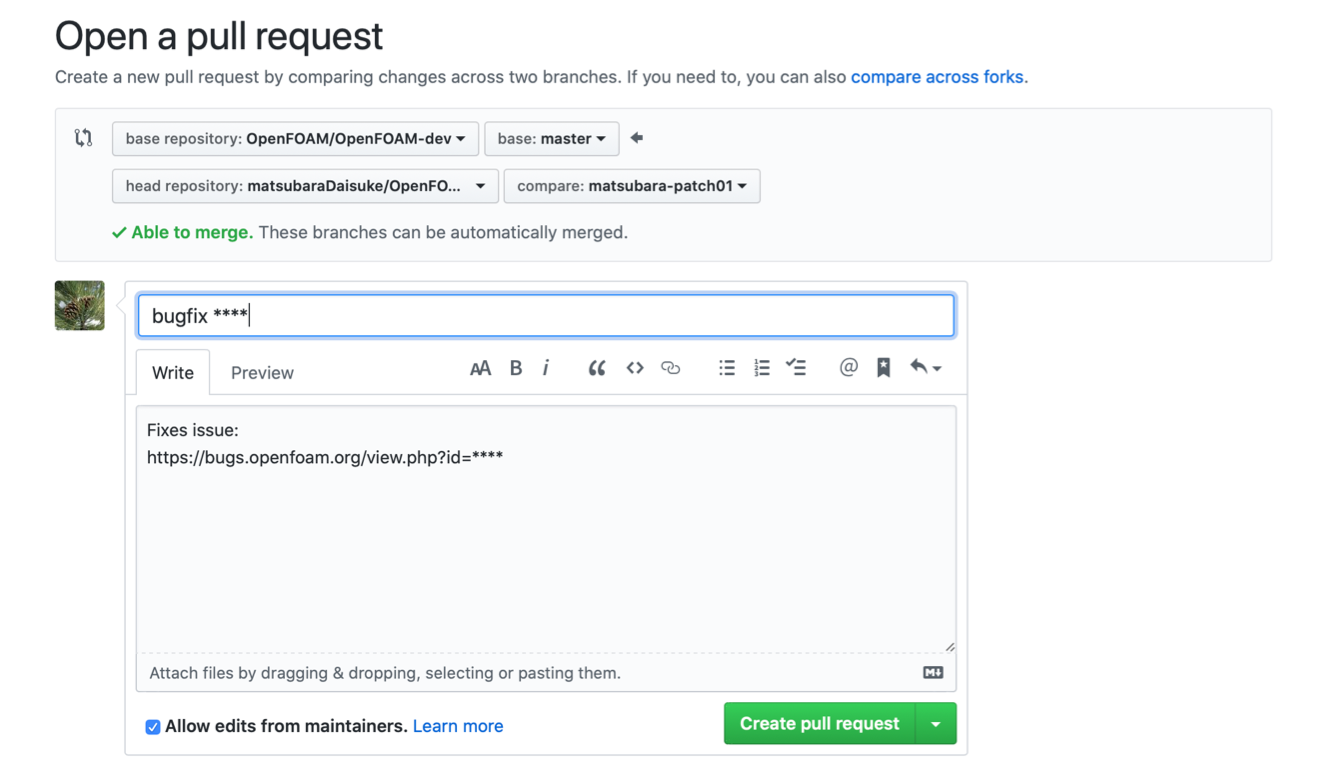
\includegraphics[width=5cm]{fig/fig-f5.png}
\begin{figure}[htbp]
\centering
\subfigure[Pull request your branch into the master branch.]{
  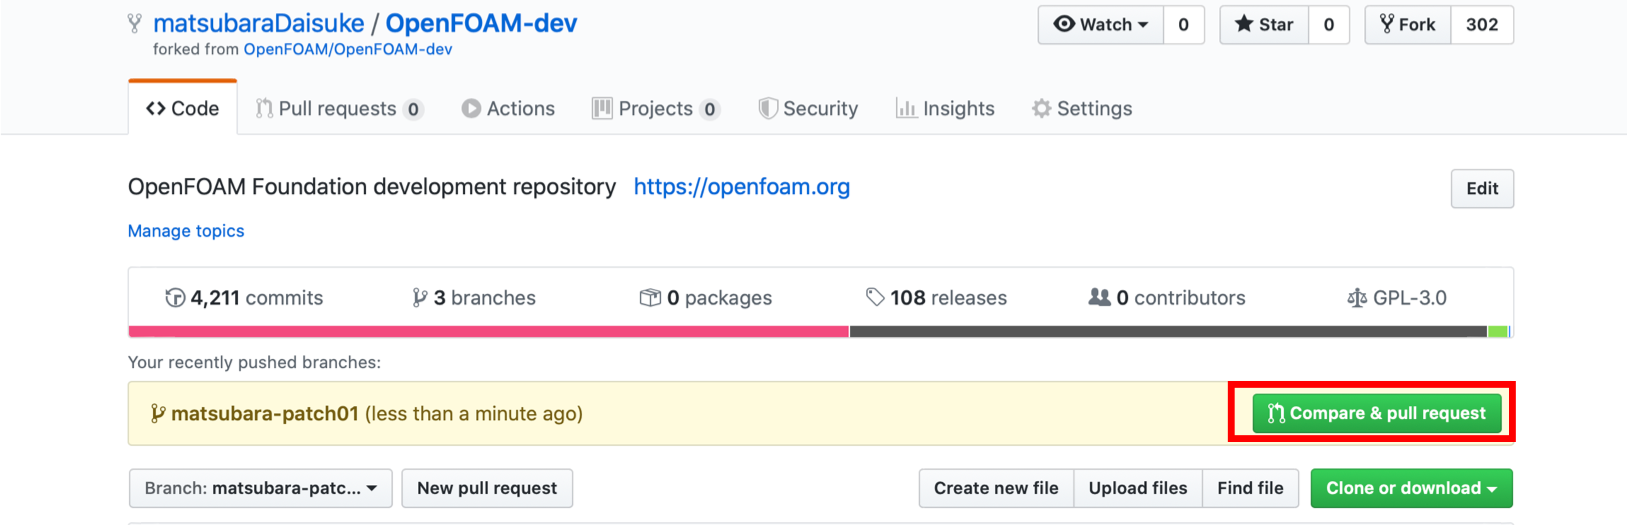
\includegraphics[width=0.8\textwidth]{fig/fig-f4.png}
  \label{fig:f4}
}
%\hspace{0.1\textwidth}
\subfigure[Add your message to pull request.]{
  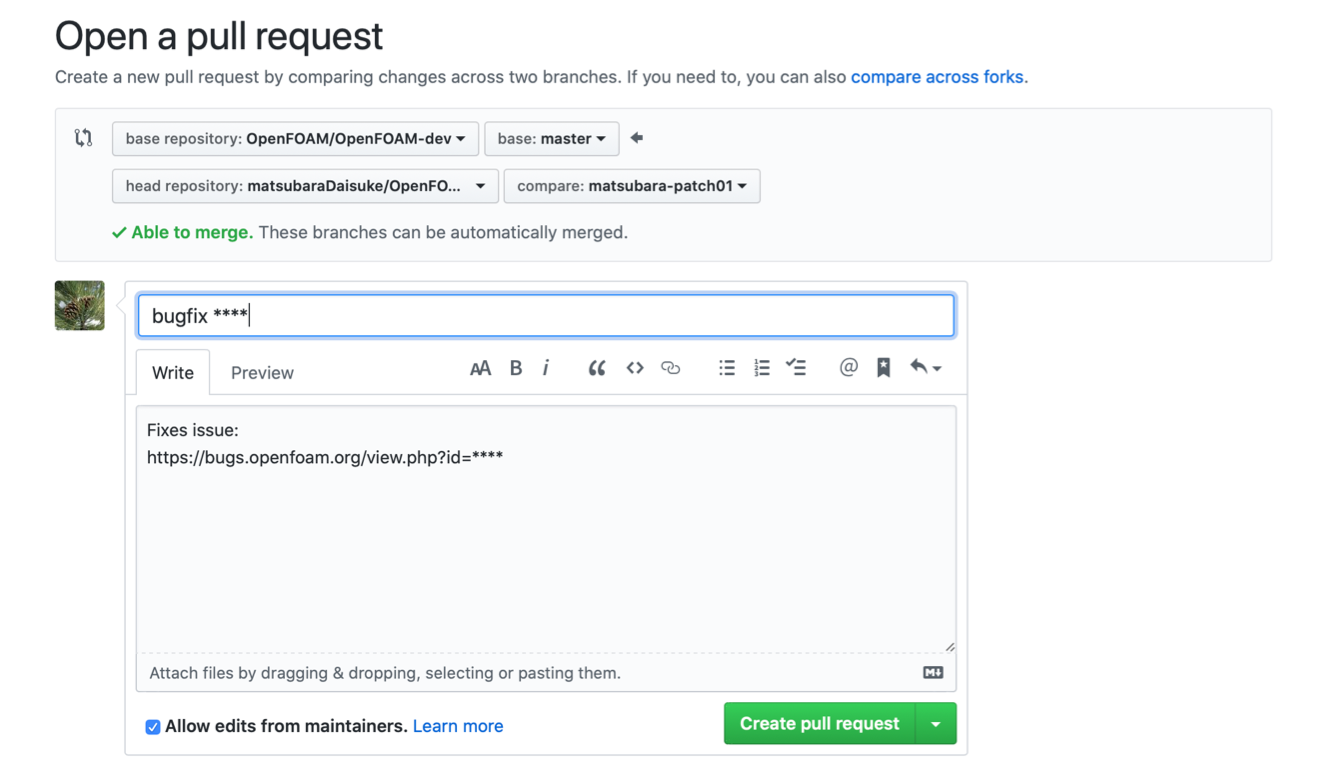
\includegraphics[width=0.8\textwidth]{fig/fig-f5.png}
  \label{fig:f5}
}
\caption{A explication to pull request your branch into the master branch.}
\label{fig:f4f5}
\end{figure}


\section{Gitの使い方}
本節では https://github.com/OpenFOAM-jp/OpenFOAM-jp.git 
のリポジトリにコントリビュートの練習をする方法について解説する.
環境はUbuntu18.04の環境を想定する.
事前に{GitHub}のアカウントを作成する必要がある.
コントリビュートをする際にはまず,Issueを立て自分が加えたい変更について議論する.
Issueを立てる際には以下の内容が含まれていることが望ましい.
\begin{itemize}
  \item 機能の簡単な説明.問題が何であるかの明確で簡潔な説明.
  \item 希望するソリューションの説明.あなたが何をしたいのかについての明確で簡潔な説明.
  \item 検討した代替案を説明.検討した代替ソリューションまたは機能の明確で簡潔な説明.
  \item 追加のコンテキスト.機能リクエストに関する他のコンテキストまたはスクリーンショットをここに追加します.
\end{itemize}
OSSのコントリビュートのバージョン管理ソフトにはGitが一般的に使用されている.
OpenFOAMの開発においてもGitが使用されている.
まずは,Gitをインストールする.

\begin{shbox}
  \shuser{user}
  \shline{}{sudo apt install git}
\end{shbox}

必要なのはソースだけで貢献しないのであれば,次のコマンドでcloneすることで作業は終わる.

\begin{shbox}
  \shuser{user}
  \shline{}{git clone https://github.com/OpenFOAM-jp/OpenFOAM-jp.git}
\end{shbox}

貢献をしたい場合は,OpenFOAM-jpのリポジトリを自分のアカウントにForkする.

TODO: Forkの際の画面キャプチャを挿入する.

Fork後は自分のアカウントのリポジトリをcloneする.

\begin{shbox}
  \shuser{user}
  \shline{}{git clone https://github.com/your\_account\_name/OpenFOAM-jp.git}
\end{shbox}

cloneをしたら自分の環境で実行環境を構築する.
まずは,OpenFOAMを動かすために必要な外部ライブラリをインストールする.

\begin{shbox}
  \shuser{user}
  \shline{}{sudo apt update}
  \shline{}{sudo apt upgrade}
  \shline{}{sudo apt install git-core}
  \shline{}{sudo apt install build-essential}
  \shline{}{sudo apt install cmake}
  \shline{}{sudo apt install libfl-dev}
  \shline{}{sudo apt install bison}
  \shline{}{sudo apt install zlib1g-dev}
  \shline{}{sudo apt install qt4-dev-tools}
  \shline{}{sudo apt install libqt4-dev}
  \shline{}{sudo apt install libqtwebkit-dev}
  \shline{}{sudo apt install gnuplot}
  \shline{}{sudo apt install libreadline-dev}
  \shline{}{sudo apt install libncurses-dev}
  \shline{}{sudo apt install libxt-dev}
  \shline{}{sudo apt install libopenmpi-dev}
  \shline{}{sudo apt install openmpi-bin}
  \shline{}{sudo apt install libboost-system-dev}
  \shline{}{sudo apt install libboost-thread-dev}
  \shline{}{sudo apt install libgmp-dev}
  \shline{}{sudo apt install libmpfr-dev}
  \shline{}{sudo apt install python}
  \shline{}{sudo apt install python-dev}
  \shline{}{sudo apt install libcgal-dev}
  \shline{}{sudo apt install curl}
  \shline{}{sudo apt install git-core}
  \shline{}{sudo apt install build-essential}
  \shline{}{sudo apt install cmake}
  \shline{}{sudo apt install libfl-dev}
  \shline{}{sudo apt install bison}
  \shline{}{sudo apt install zlib1g-dev}
  \shline{}{sudo apt install qt4-dev-tools}
  \shline{}{sudo apt install libqt4-dev}
  \shline{}{sudo apt install libqtwebkit-dev}
  \shline{}{sudo apt install gnuplot}
  \shline{}{sudo apt install libreadline-dev}
  \shline{}{sudo apt install libncurses-dev}
  \shline{}{sudo apt install libxt-dev}
  \shline{}{sudo apt install libopenmpi-dev}
  \shline{}{sudo apt install openmpi-bin}
  \shline{}{sudo apt install libboost-system-dev}
  \shline{}{sudo apt install libboost-thread-dev}
  \shline{}{sudo apt install libgmp-dev}
  \shline{}{sudo apt install libmpfr-dev}
  \shline{}{sudo apt install python}
  \shline{}{sudo apt install python-dev}
  \shline{}{sudo apt install libcgal-dev}
  \shline{}{sudo apt install curl}
\end{shbox}

次に,OpenFOAMのbashrcをターミナル起動時に読み込むように~/.bashrcに登録する.

\begin{shbox}
  \shuser{user}
  \shline{}{echo "source ~/OpenFOAM/OpenFOAM-dev/etc/bashrc" >> ~/.bashrc}
  \shline{}{. ~/.bashrc}
\end{shbox}

ThirdPartyの中のParaViewをインストールする.
この際にpythonを登録するとParaViewのpython拡張機能が使用可能になる.
既にParaViewをインストールしている場合であっても,このParaViewはOpenFOAMの結果表にのプラグインなども同梱しているため,
以下の手順でもう一つインストールすることを推奨する.

\begin{shbox}
  \shuser{user}
  \shline{}{cd \$WM\_THIRD\_PARTY\_DIR}
  \shline{}{./makeParaView -python -python-lib /usr/lib/x86\_64-linux-gnu/libpython2.7.so.1.0}
\end{shbox}

最後にOpenFOAMをインストールする.

\begin{shbox}
  \shuser{user}
  \shline{}{wmRefresh}
  \shline{}{cd \$WM\_PROJECT\_DIR}
  \shline{}{./Allwmake -j | tee log.Allwmake}
\end{shbox}

ソルバーを動かしてインストールの確認を行う.

\begin{shbox}
  \shuser{user}
  \shline{}{mkdir \$WM\_PROJECT\_USER\_DIR}
  \shline{}{cd \$WM\_PROJECT\_USER\_DIR}
  \shline{}{cp -r \$FOAM\_TUTORIALS/basic/potentialFoam/pitzDaily/ ./}
  \shline{}{cd pitzDaily/}
  \shline{}{foamRunTutorials}
  \shline{}{paraFoam}
\end{shbox}

これでParaViewが起動されて結果の表示ができたら完成である.
テストが全てパスしたらソースを変更する.
masterブランチで直接変更することはできないため,ファイルを変更する前に開発ブランチを作成する.

\begin{shbox}
  \shuser{user}
  \shline{}{git branch branch\_name}
\end{shbox}
\begin{shbox}
  \shuser{user}
  \shline{}{git checkout branch\_name}
\end{shbox}

branch\_name には任意の名前を入れる.
自分のアカウント名と加えたい変更について言及されていると分かりやすい.
最初のコマンドでブランチを作成し,2番目のコマンドでブランチに移動する.
これにより,変更を行う準備はほぼ完了である.
変更のラベルを付けるために,連絡先の名前と電子メールを以下のコマンドで指定する.

\begin{shbox}
  \shuser{user}
  \shline{}{git config --global user.name "Your Name Comes Here"}
  \shline{}{git config --global user.email you@yourdomain.example.com}
\end{shbox}

もし src/toto.cc というファイルをいくつか変更したり,新しいファイルとして追加したら,
ローカルのコミットは次のコマンドで行う.
"Your extensive commit message here \#1" には変更に関するメッセージを追加する.
\#1の部分は自分が追加したイシューの番号とする.

\begin{shbox}
  \shuser{user}
  \shline{}{git add src/toto.cc}
  \shline{}{git commit -m "Your extensive commit message here \#1"}
\end{shbox}

この段階ではコミットはあなたのローカルリポジトリで行われていますが,GitHubリポジトリでは行われない.
十分なテストで変更を検証したら,以下のコマンドでGitHubの自分のアカウントのリポジトリに変更を移すことができる.

\begin{shbox}
  \shuser{user}
  \shline{}{git push origin branch\_name}
\end{shbox}

TODO: コマンドのメッセージを含める

このコマンドのメッセージに図のようなURLが表示される.
URLにアクセスしプルリクエストを作成する.

TODO: GetFEMのドキュメントから引用を行っているため言及する.

GetFEM++ のマスターブランチにマージすることは許可されていないので,あなたの役割はここで終わる.
プルリクエストのページで管理者や他の開発者と議論することができる.
管理者が承認した場合には変更がマージされる.

いくつかの便利なgitコマンドを示す.

\begin{shbox}
  \shuser{user}
  \shline{}{git status  : status of your repository / branch}
  \shline{}{git log --follow "filepath"   : Show all the commits modifying the specified file (and follow the eventual change of name of the file).}
  \shline{}{gitk --follow filename : same as previous but with a graphical interface}
\end{shbox}

\section{GitHub および Travis による継続的インテグレーション}
Travis CIは,GitHub上のソフトウェアのビルドやテストを行う,オンラインで分散型の継続的インテグレーション (CI) サービスである.
継続的インテグレーションサービスとは,ビルドやテストを継続的に自動実行するサービスである.
継続的インテグレーションを行うことにより,機能追加やリファクタリングによるデグレードを防ぐことができる.
以下に,GetFEM++で使用している.travis.ymlを示す.
リポジトリにymlファイルを追加することで,Travisによるインテグレーションテストが実行される.
今後OpenFOAMのリポジトリでもCIが実行できるようにする予定である.
\begin{lstlisting}
language: python
python:
  - "3.6"
sudo: false
dist: bionic
cache:
  directories:
  - $HOME/.cache/pip
before_install:
- sudo apt-get install -y --no-install-recommends automake
- sudo apt-get install -y --no-install-recommends libtool
- sudo apt-get install -y --no-install-recommends make
- sudo apt-get install -y --no-install-recommends g++
- sudo apt-get install -y --no-install-recommends libqd-dev
- sudo apt-get install -y --no-install-recommends libqhull-dev
- sudo apt-get install -y --no-install-recommends libmumps-seq-dev
- sudo apt-get install -y --no-install-recommends liblapack-dev
- sudo apt-get install -y --no-install-recommends libopenblas-dev
- sudo apt-get install -y --no-install-recommends libpython3-dev
- sudo apt-get install -y --no-install-recommends ufraw
- sudo apt-get install -y --no-install-recommends imagemagick
- sudo apt-get install -y --no-install-recommends fig2dev
- sudo apt-get install -y --no-install-recommends texlive
- sudo apt-get install -y --no-install-recommends xzdec
- sudo apt-get install -y --no-install-recommends fig2ps
- sudo apt-get install -y --no-install-recommends gv
- pip install -r requirements.txt
addons:
  apt:
    update: true
script:
- bash autogen.sh
- export CXXFLAGS=-coverage
- export LDFLAGS=-coverage
- export CPPFLAGS=-coverage
- export CFLAGS=-coverage
- export FCFLAGS=-coverage
- ./configure --with-pic
- make -j8
- make -j8 check
- (cd doc/sphinx; make html)
after_success:
- bash <(curl -s https://codecov.io/bash)
\end{lstlisting}

TODO Travis CIについてWikipediaからの引用であることを明記する.

TODO 継続的インテグレーションサービスについてWikipediaからの引用であることを明記する.
%
\section{OpeFOAM-jp}
OpenFOAM-jp\cite{URL:OpenFOAM-jp}は今回立ち上がったコミュニティの活動を行うためのGiuHubレポジトリである.
目的は日本のOpenFOAMコミュニティの活性化,OpenFOAMへのコントリビュートの入り口,およびOSSコントリビュート活動の学習の場としている.
参加は誰でも国籍を問わず可能であり,今後人口が増えてオープンで有意義な場として機能することを期待する.
%
\subsection{OpenFOAM-jp/issues}
issuesレポジトリ\cite{URL:OpenFOAM-jp-issues}は最初の議論を行う場として設置された.
テキストエディタVimの日本コミュニティのレポジトリ\cite{URL:vim-jp}のForkであり,運用方法もこれを参考にする.
ここではOpenFOAMの新機能の提案やOpenFOAM-jpで行う活動の議論などを行うことを目的としている.
質問掲示板であるGoogle Forumと役割が重複すると混乱や情報の偏りを発生させるため明確な差別化を行うように注意して運用していく.
%
\subsection{OpenFOAM-jp/OpenFOAM-jp}
OpenFOAM-jpレポジトリ\cite{URL:OpenFOAM-jp-OpenFOAM-jp}はFoundation版のOpenFOAM-devのForkであり,pushやPull Requestなどのgitの基本機能の練習用に設置された.
branchを作成してオリジナルの機能を配布する目的で使用することも期待している.
エラーメッセージの日本語化プロジェクトなども予定している.
%
\subsection{OpenFOAM-jp/OpenFOAM-utilities-tutorials-jp}
OpenFOAM-utilities-tutorials-jp\cite{URL:OpenFOAM-jp-OpenFOAM-utilities-tutorials-jp}は,web上にあまり情報のないOpenFOAMのutilitiesに関するまとめを行う目的で設置された.
その一例を\autoref{fig:utilities-example}に示す.
\begin{figure}[htbp]
\centering
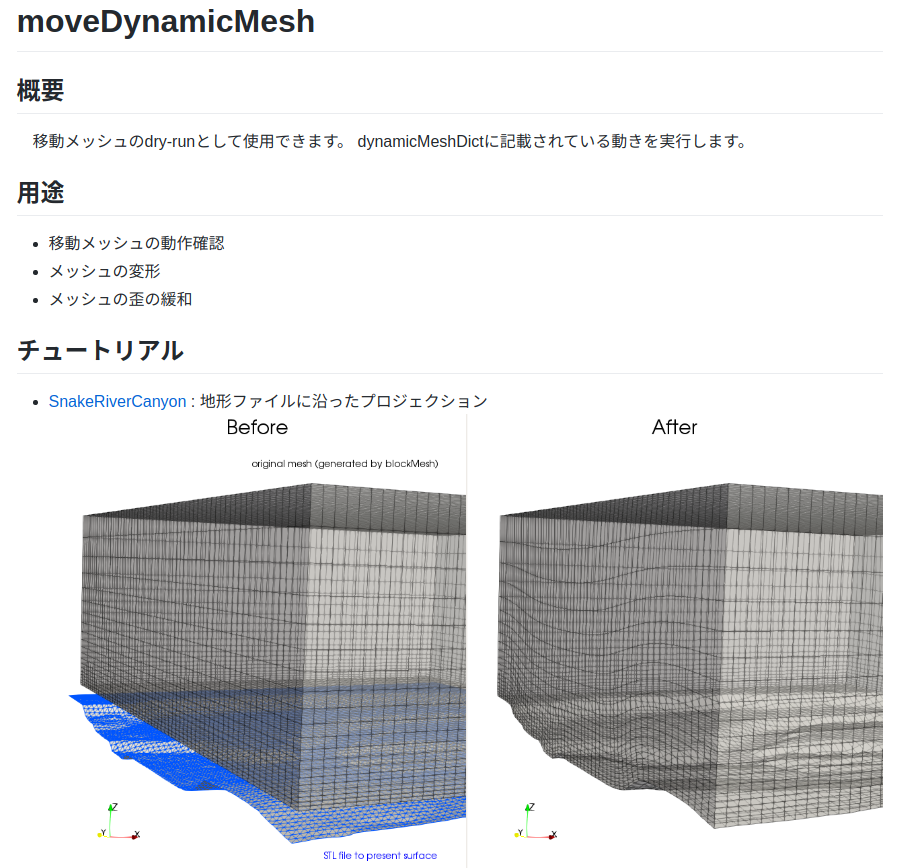
\includegraphics[width=0.8\textwidth]{fig/utilities-example.png}
\caption{moveDynamicMesh(v1906) utilitiy's tutorial document.\cite{URL:OpenFOAM-jp-movedDynamicMesh}}
\label{fig:utilities-example}
\end{figure}
各utilityについて,使用方法をMarkDown形式のドキュメントでまとめ,そのチュートリアルを作成する.
ディレクトリ構成は実際のソースコードに準拠し,最表層のMarkDownファイルから各ドキュメントにアクセスできるようにしている.\cite{URL:OpenFOAM-jp-util-index}
現時点ではOpenFOAM-v1906について作成中である.
%
\section{まとめ}

%%%
%%% OpenCAEシンポジウムTeXテンプレートファイル
%%% OpenFAOM-jp_OpenCAE_symposium.tex
%%% OpenCAEシンポジウム2018版
%%%
%%
%% ltjocはOpenCAE論文集・シンポジウム用のクラスファイルです.変更しないでください.
%% 本文が英語の場合には,オプションにenglishを指定してください.
\documentclass{ltjoc}
%\documentclass[english]{ltjoc}
\usepackage[
 backgroundcolor=gray!50,
 usernamecolor=black,
 machinenamecolor=black,
 indicatorcolor=black,
 separatorcolor=black,
 pathcolor=black,
 optioncolor=black,
 textcolor=black
]{shdoc}
%%
%% 表題(title),副題(subtitle),著者(author),所属(affiliation)
%% 本文が英語の場合には,こちらに英文表題,英文副題,英文著者,英文所属を記述します.
\title{OpenFOAMコントリビュート活動}
% 副題が無い場合にはコメントアウトします.
% \subtitle{\TeX のテンプレート(和文副題)} 
\author{%
稲葉竜一$^{1\dagger}$%
\hspace{1\zw}%
松原 大輔$^{2}$%
\hspace{1\zw}%
@tkoyama010$^{1}$%
}
\affiliation{%
${}^{1}$OpenFOAM-jp%
\hspace{1\zw}%
${}^{2}$オープン CAE勉強会%
} 
%%
%% Corresponding authorの電子メールアドレス
%% 本論文について連絡が取れる著者の電子メールアドレスを記載してください.
\AuthorsEmail{inabower@gmail.co.jp}
%%
%% 英文表題(etitle),英文副題(esubtitle),英文著者(eauthor),英文所属(eaffiliation)
%% 本文が英語の場合には表示されません.
\etitle{OpenFOAM Contributing Activities}
% 副題が無い場合にはコメントアウトします.
% \esubtitle{The case of \TeX (English Sub-Title)}
\eauthor{%
Ryuichi INABA$^{*\dagger}$%
\hspace{1em}%
Daisuke MATSUBARA$^{**}$%
\hspace{1em}%
@tkoyama010$^{*}$%
}
\eaffiliation{%
${}^{*}$OpenFOAM-jp%
\hspace{1em}%
${}^{**}$OpenCAE Local user group%
}
%%
%% キーワード
\keywords{GitHub, git, Pull Request, OpenFOAM, develop}
%%
%% 英文概要
%% 英文概要を省略する場合には,abstract環境の定義をしないでください.
\begin{abstract}
Commits from Japanese to OpenFOAM are less.
So, we established a group called OpenFOAM-jp by volunteers.
We started contributing activities such as development of software,
translation of documents and preparation of tutorials.
We will report how to join our activity by using git and GitHub.
\end{abstract}
%%
%% luatexja-fontspecパッケージ
\usepackage{luatexja-fontspec}
\defaultfontfeatures{Ligatures=TeX}
%% luatexja-presetパッケージ
%% 和文フォントのプリセット設定
%% オプションにnoembed(非埋込)を指定しないでください.
%\usepackage[ipaex]{luatexja-preset} % IPAex(デフォルト)
%\usepackage[ms]{luatexja-preset} % MS
%\usepackage[hiragino-pro]{luatexja-preset} % ヒラギノPro
%%
%% 欧文フォントの指定
%% 使用できるフォントについては,以下のコマンドで調べてください.
%% $ luaotfload-tool --list=*
%%
%% 欧文通常フォント
%\setmainfont{Cambria} % Cambria
%\setmainfont{Times New Roman} % Times New Roman
%\setmainfont{TeXGyreTermes} % TeXGyreTermes
%%
%% 欧文Sans-serifフォント
%\setsansfont{Calibri} % Calibri
%\setsansfont{Arial} % Arial
%\setsansfont{Helvetica} % Helvetica
%\setsansfont{TeXGyreHeros} % TeXGyreHeros
%%
%% 欧文monospaceフォント
%\setmonofont{Consolas} % Consolas
%\setmonofont{Courier New} % Courier New
%\setmonofont{Lucida Console} % Lucida Console
%%
%% subfigureパッケージ
\usepackage{subfigure}
%%
%% graphicxパッケージ
\usepackage{graphicx}
%%
%% hyperrefパッケージ
\usepackage[
 pdfencoding=auto,
 bookmarks=true,
 bookmarksnumbered=true,
 colorlinks=true,
 allcolors={blue}
]{hyperref}
%%
%% listingsパッケージ
\usepackage{listings}
\renewcommand{\lstlistingname}{Code}
\lstset{
basicstyle={\footnotesize\ttfamily},
commentstyle=\color{blue},
frame={tb},
breaklines=true,
columns=[l]{fullflexible},
numbers=left,
numberstyle={\footnotesize},
keepspaces=true
}
%%
%% autorefでの図表の参照名の再定義
\makeatletter
\if@english
  \renewcommand*{\figureautorefname}{\figurename}
  \renewcommand*{\tableautorefname}{\tablename}
\else
  \renewcommand*{\figureautorefname}{図}
  \renewcommand*{\tableautorefname}{表}
\fi
\makeatother
%%
%% ヘッダ右の設定
%% 変更しないでください.
\markright{Open CAE Symposium 2019, Dec. 19-21, 2019, Osaka, D-2} % Do not edit this line
%%
%% 本文
\begin{document}
%%
%% 題目などの出力
\maketitle
%%%
\section{はじめに}
現状日本からのOpenFOAMへのコントリビュートは少ない.
そこで有志により"OpenFOAM-jp"といグループを立ち上げ,本家の開発やドキュメントの翻訳,チュートリアルの作成などのコントリビュート活動を始めた.
本報告ではその活動内容などについて発表する.
\section{Foundation版とESI版の違い}
OpenFOAMは,Imperial Collageで開発された商用CFDコードFOAM(Field Operation And Manipulation)が,2004年にOpenFOAMと名前を変えてオープンソースとしてリリースされたことから始まる.\cite{URL:openfoam.history}\cite{Minabe:OpenCAE2015-GP23}
2011年にはOpenFOAMを運営しているOpenCFD社がSGI社に買収され,またその2社によりOpenFOAMの商標を譲渡したOpenFOAM Foundation Inc.を設立した.
これ以降OpenFOAMはOpenFOAM Foundation Inc.より開発と配布が行われており,2019年11月現在OpenFOAM-V7を最新版とするForkが”Foundation版”\cite{URL:openfoam.org}\cite{URL:GitHub-foundation}と呼ばれている.

一方でOpenFOAMには多くのForkが存在する.
2012年以降はESI社がOpenCFD社の買収という形から開発に加わるようになり,
2016年にはOpenFOAM-v3.0からForkしたOpenFOAM-v3.0+をリリースした.
2019年11月時点ではこの最新版はOpenFOAM-v1906であり,このForkが”ESI版”\cite{URL:openfoam.com}\cite{URL:GitLab-plus}もしくは”plus版”と呼ばれる.

本報告ではこのFoudation版とESI版の2つについてコントリビュートの流れなどを報告する.
%
\section{ESI版コントリビュート方法}
ESI版の開発はGitLabで行われている.\cite{URL:GitLab-plus}
このページからレポジトリをcloneすることができ,これをそのままコンパイルすることで次期リリース予定のESI版OpenFOAMを使用することができる.
またここには開発途中のbranchが多くあり,将来的に追加されるであろう機能をチェックすることもできる.

\autoref{fig:plus-register}に示すGitLabのページの右上のボタンからこのOpenFOAM-plusのレポジトリに登録することもでき,これによりissueの作成や書き込みをすることができるようになる.
\begin{figure}[htbp]
\centering
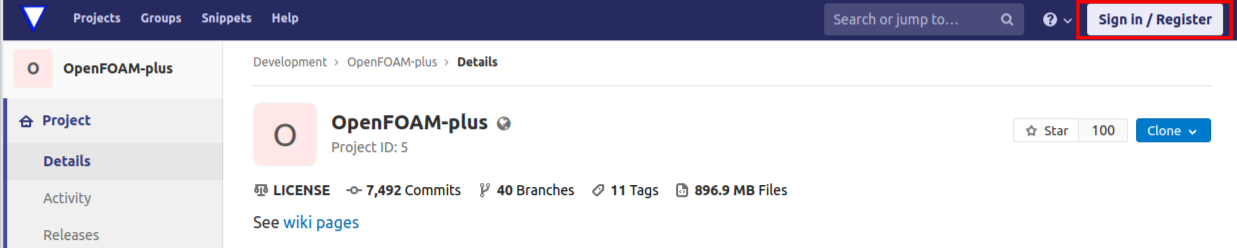
\includegraphics[width=0.8\textwidth]{fig/plus_register.png}
\caption{A register button of OpenFOAM-plus's GitLab page.}
\label{fig:plus-register}
\end{figure}
例えばバグを見つけた場合やOpenFOAMへの要望がある場合には,issueを作成することで開発者へ周知することができ,必要と判断された場合には開発者によりコードの修正や作成が行われる.
\autoref{fig:plus-issue}には実際に作成したissueの例を示す.内容としてはソルバーのDiscriptionの中のスペルミスを指摘した簡単なものであるが,数日以内に@mark氏により該当箇所の修正が行われていることが確認できる.
\begin{figure}[htbp]
\centering
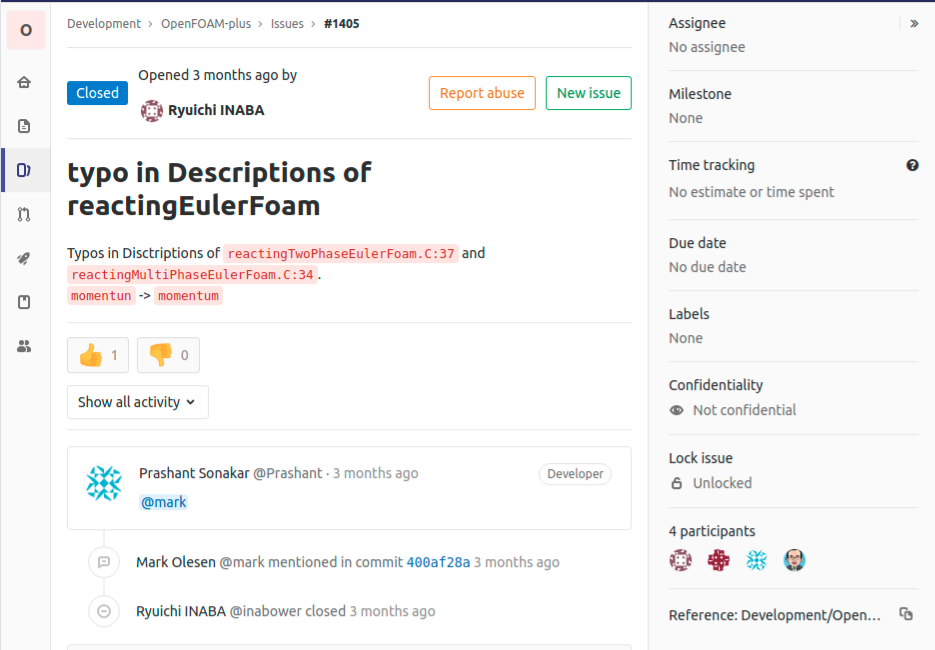
\includegraphics[width=0.8\textwidth]{fig/plus_issue.png}
\caption{An Example issue to fix typo.}
\label{fig:plus-issue}
\end{figure}
このような小さなコントリビュートの積み重ねがOSSであるOpenFOAMを精錬していくこととなる.

一方で,pushやPull Requestなどのコードの変更を行うための権限は制限されている.
このため,ESI版OpenFOAMのコードにコントリビュートする手段としては,開発メンバーに加わらない限りはissueの作成もしくはissue内の議論へ参加することに限られる.
なお2019年11月現在OpenFOAM-plusの開発メンバーは15名であり,実力や面識,貢献頻度が担保されたメンバーで開発を行っていることが推察される.\cite{URL:GitLab-plus-members}
%
\section{Foundation版コントリビュート方法}

Foundation版の開発はGithubで行われている.Foundation版ではissueの管理はGithubでは行わないので注意が必要である.バグ報告は専用のissueTrackingのページへ登録する必要がある.
未登録の場合は,名前とメールアドレスを入力し,返信のリンクを辿ることでviewerとして参加することができる.
また数時間後にスパムでないことが認められると,reporterに昇格できる.
reporterとなることでissueを立てて,バグの報告が可能となる.
ここでバグの重要度や改善方法を議論をすることになる.
issueTrackingの内容を確認すると,Foundation版は基本的にbugfixを目的としたコントリビュートが主の様である.

重大なバグの修正または,新しい開発を提供する場合,OpenFOAM Foundation Contributor Agreementに署名する必要がある.
Foundation版HPのメニューバーのDevelopment/ContributorAgreeementのリンクを辿り,Contact Usのページから名前と所属,コントリビュートに参加した意思を記載して送信すると,後日,Henry G. WellerからPDF形式の登録用紙が送付されてくる.
登録用紙の内容は,前述のContributorAgreeementのページに記載されているものと同じである.

バグの修正などでFoundation版のOpenFOAMの修正を開発元に共有する場合,Foundation版のOpenFOAMはgithub上で管理されているため,githubアカウントが必要となる.

コントリビュートで最初に行うことは開発元のリポジトリをForkすることから始まる.(\autoref{fig:f1})
Forkしたことにより,自身のgithubアカウントにOpenFOAMのリポジトリが作成されていることが確認できる.
次に開発用の新しいブランチを作成する.ブランチ名は「(開発者名)-patch***」などとするとよいだろう.今回の例では「matsubara-patch1」とした.(\autoref{fig:f2})

\begin{figure}[htbp]
\centering
\subfigure[A fork button of Github page]{
  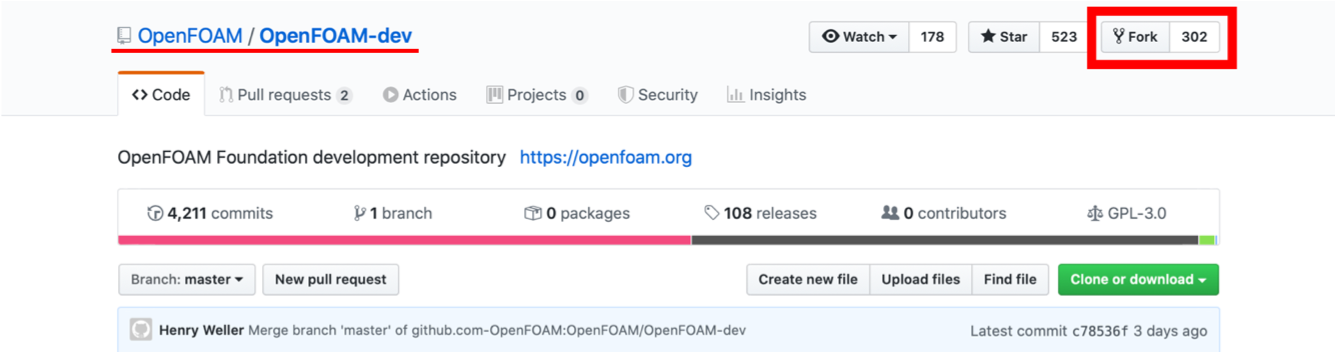
\includegraphics[width=0.8\textwidth]{fig/fig-f1.png}
  \label{fig:f1}
}
%\hspace{0.1\textwidth}
\subfigure[Creating new branch]{
  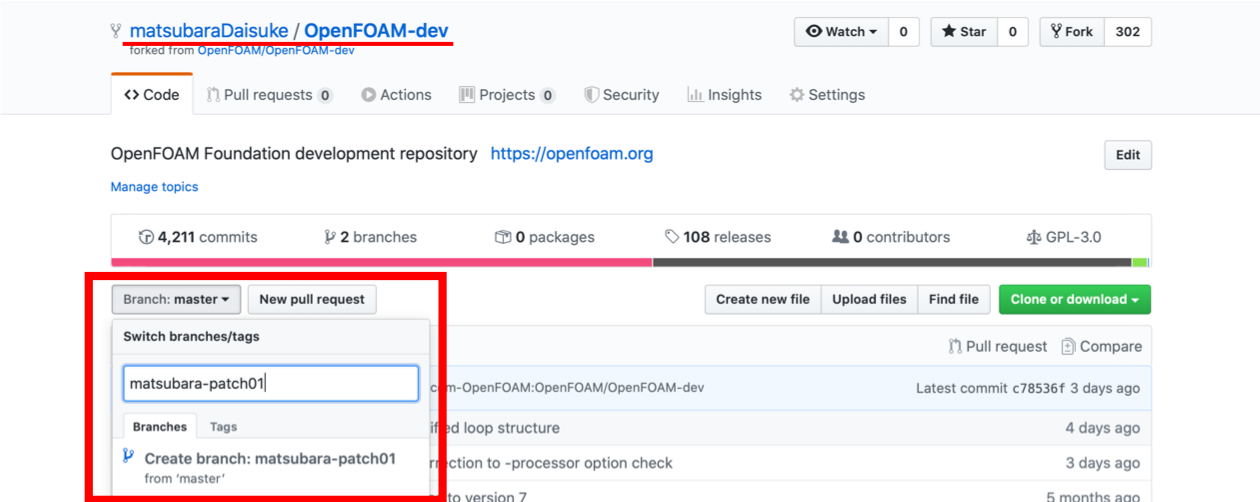
\includegraphics[width=0.8\textwidth]{fig/fig-f2.png}
  \label{fig:f2}
}
\caption{A Explication to fork OpenFOAM-dev repository and to create your new branch.}
\label{fig:f1f2}
\end{figure}
%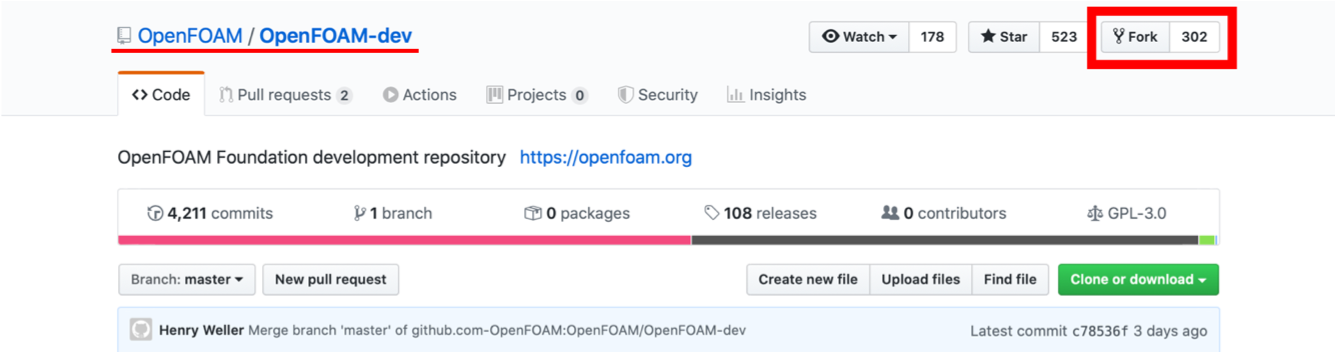
\includegraphics[width=5cm]{fig/fig-f1.png}
%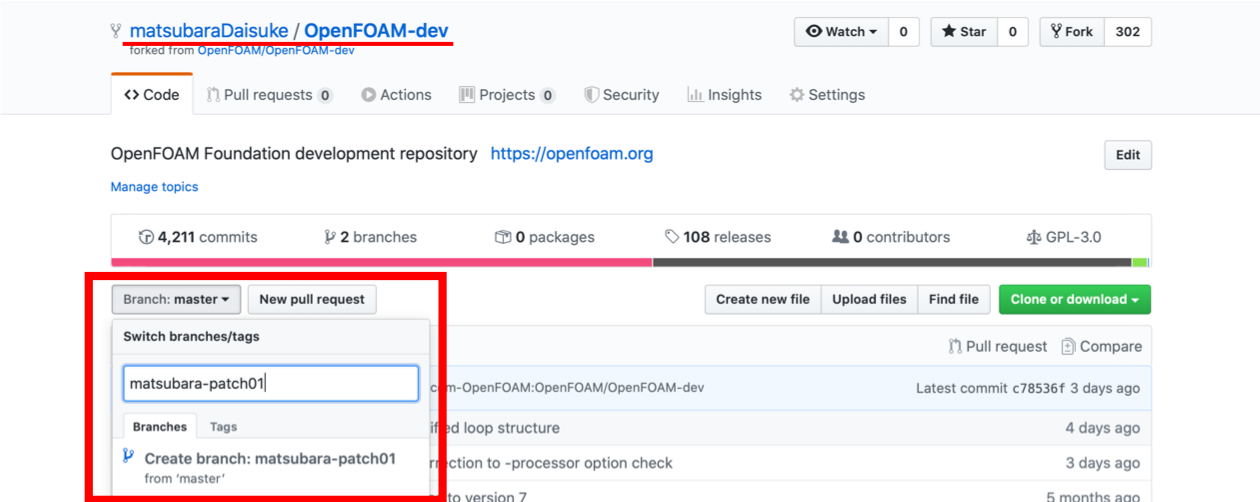
\includegraphics[width=5cm]{fig/fig-f2.png}

次に個人の開発環境に移りターミナル上でgit cloneを行う.(\autoref{fig:f3})例:git clone https://github.com/(githubアカウント名)/OpenFOAM-dev.git
これによって,git cloneしたディレクトリ下にOpenFOAMのプロジェクトがコピーされる.
%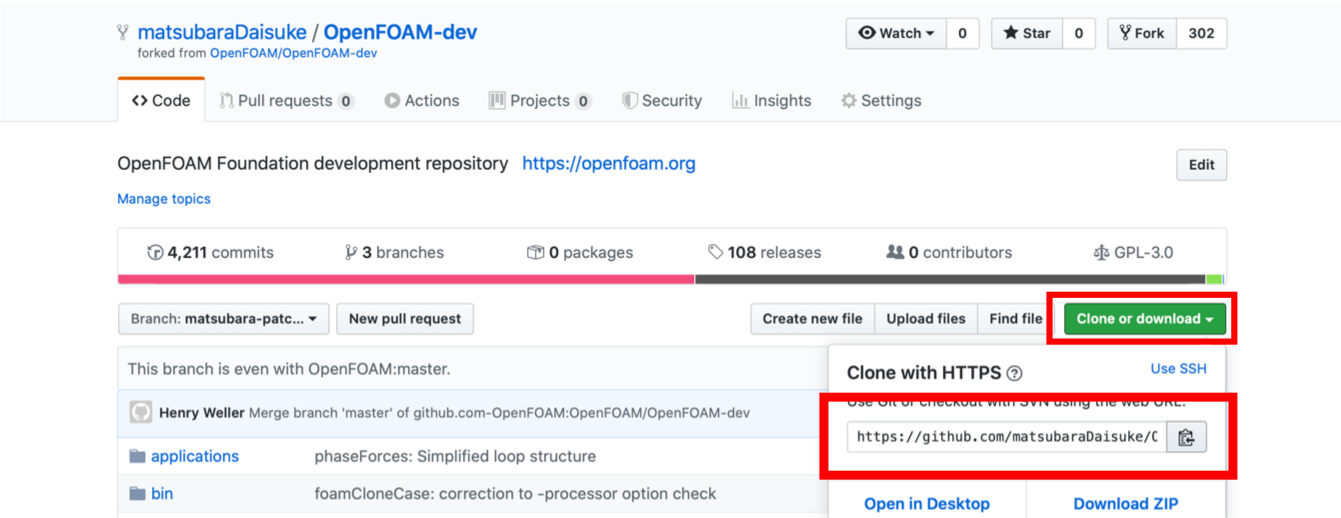
\includegraphics[width=5cm]{fig/fig-f3.png}
\begin{figure}[htbp]
\centering
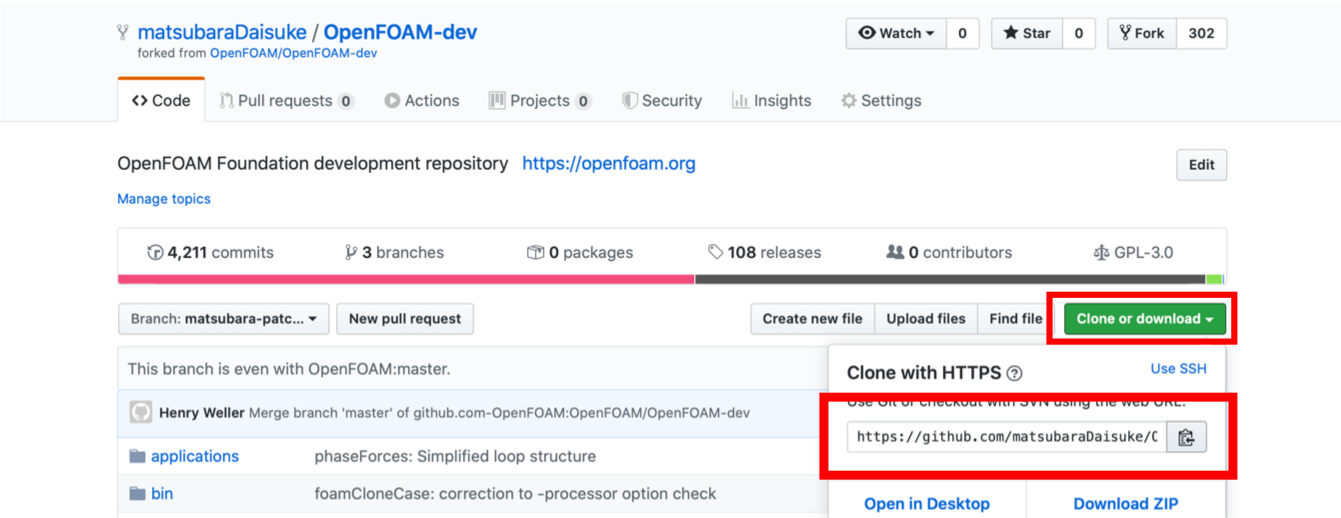
\includegraphics[width=0.8\textwidth]{fig/fig-f3.png}
\caption{Cloning repository on your local machine.}
\label{fig:f3}
\end{figure}

次にgit checkoutにて作成したブランチに切り替える 例:git checkout (開発者名)-patch***
OpenFOAMのプロジェクト内で修正や開発が完了した後,
git add . git commit -m "変更内容のコメント" git push origin (開発者名)-patch***
とすることで,コードの修正内容を個人のgithubのリポジトリに反映させる.
今回の例では以下の様な流れになる.

\begin{shbox}
  \shuser{user}
  \shline{}{git clone https://github.com/matsubaraDaisuke/OpenFOAM-dev.git}  
  \shline{}{cd OpenFOAM-dev}  
  \shline{}{git checkout matsubara-patch1}
\end{shbox}

(コーディング)

\begin{shbox}
  \shuser{user}
  \shline{}{git add .}
  \shline{}{git commit -m "bugfix ******"}
  \shline{}{git push origin matsubara-patch1}
\end{shbox}



最後にgithub上でpull requestを開発元に対して行う.(\autoref{fig:f4})この時コメントに
Fixes issue:
https://bugs.openfoam.org/view.php?id=****
の様に最初に議論したissueのURLを添付するのが慣例のようである.(\autoref{fig:f5})

%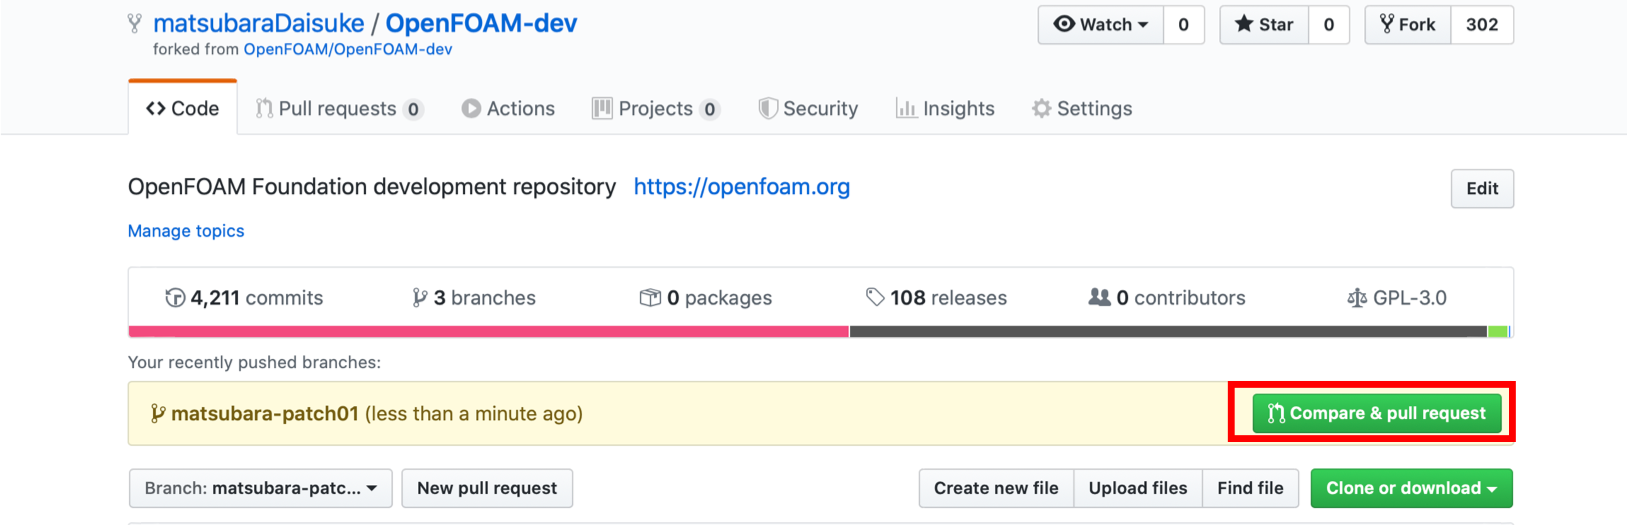
\includegraphics[width=5cm]{fig/fig-f4.png}
%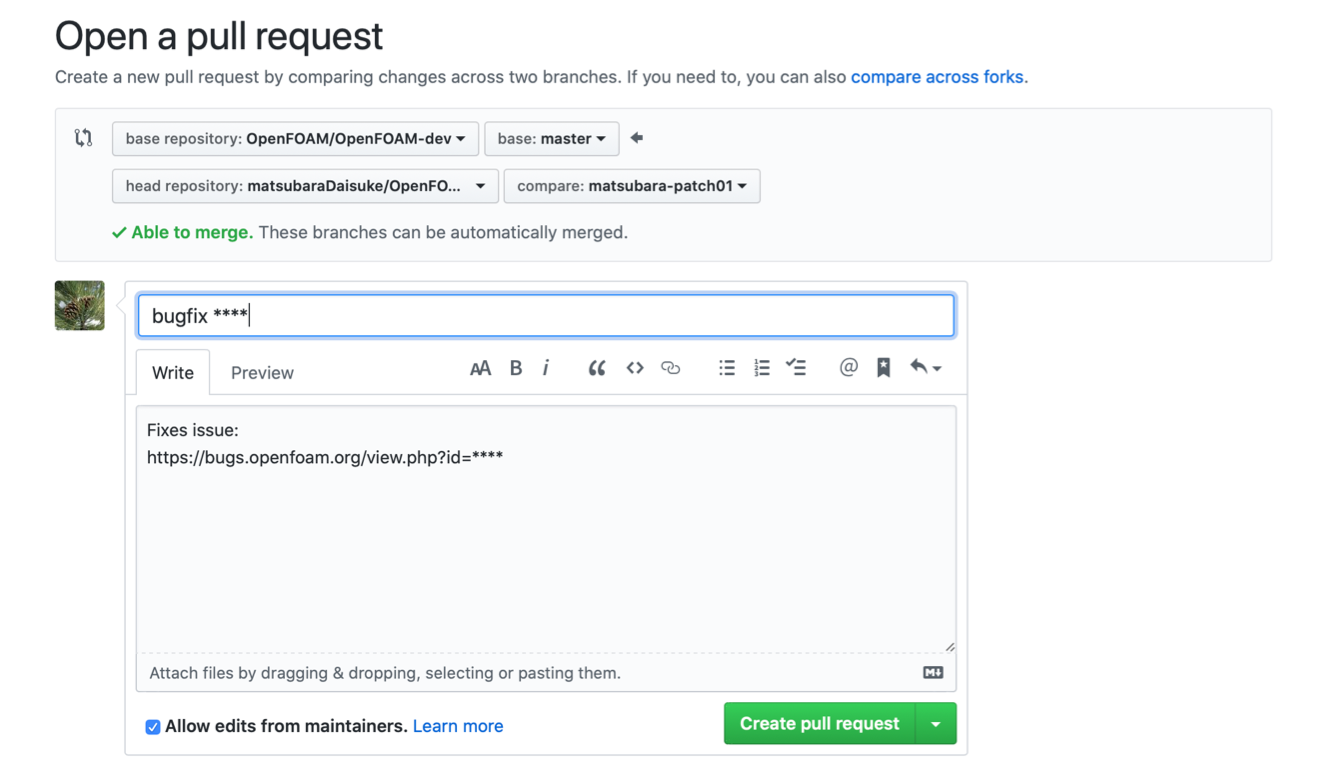
\includegraphics[width=5cm]{fig/fig-f5.png}
\begin{figure}[htbp]
\centering
\subfigure[Pull request your branch into the master branch.]{
  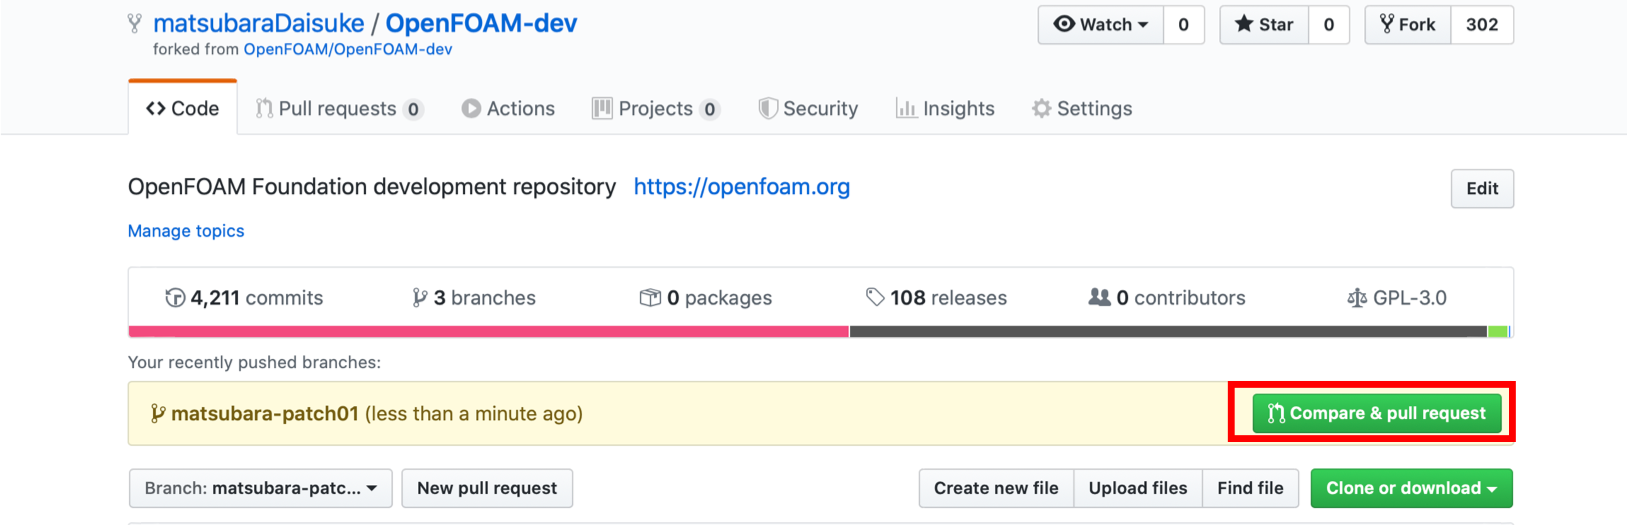
\includegraphics[width=0.8\textwidth]{fig/fig-f4.png}
  \label{fig:f4}
}
%\hspace{0.1\textwidth}
\subfigure[Add your message to pull request.]{
  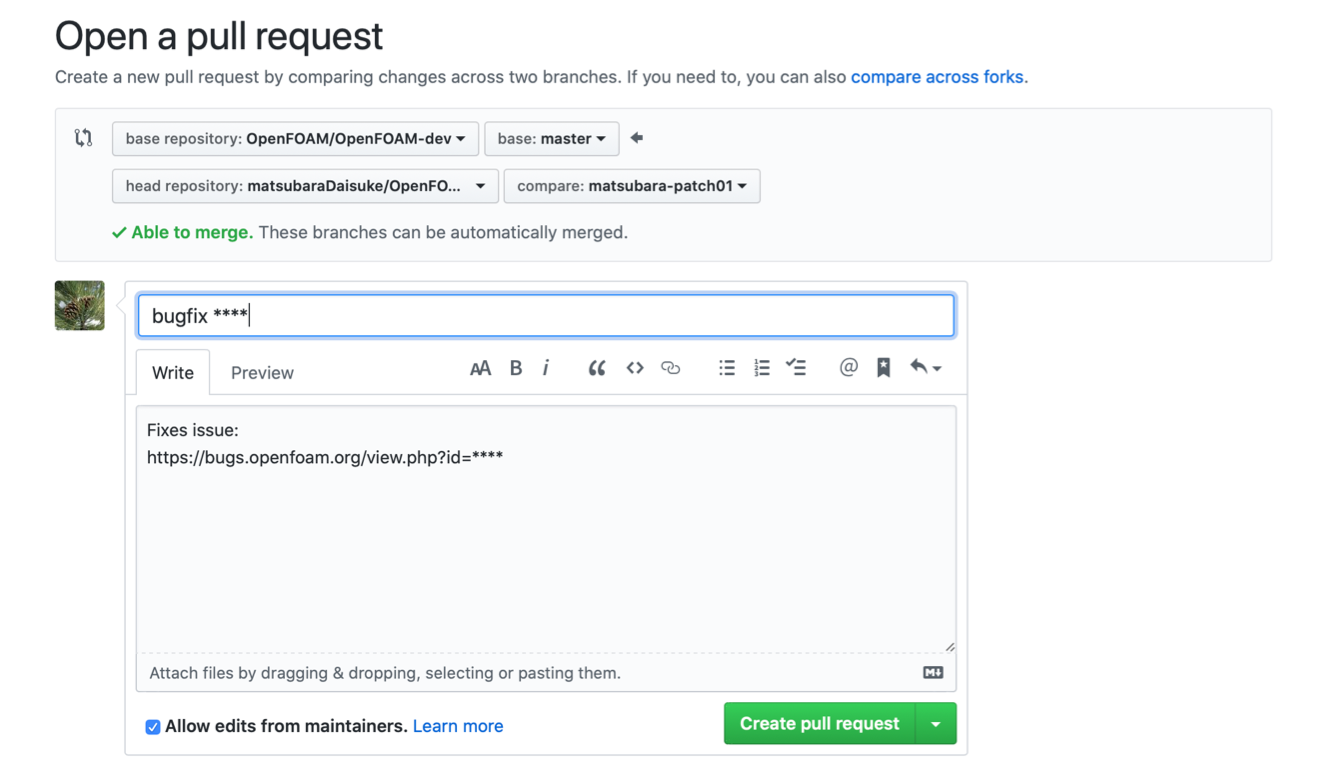
\includegraphics[width=0.8\textwidth]{fig/fig-f5.png}
  \label{fig:f5}
}
\caption{A explication to pull request your branch into the master branch.}
\label{fig:f4f5}
\end{figure}


\section{Gitの使い方}
本節では https://github.com/OpenFOAM-jp/OpenFOAM-jp.git 
のリポジトリにコントリビュートの練習をする方法について解説する.
環境はUbuntu18.04の環境を想定する.
事前に{GitHub}のアカウントを作成する必要がある.
コントリビュートをする際にはまず,Issueを立て自分が加えたい変更について議論する.
Issueを立てる際には以下の内容が含まれていることが望ましい.
\begin{itemize}
  \item 機能の簡単な説明.問題が何であるかの明確で簡潔な説明.
  \item 希望するソリューションの説明.あなたが何をしたいのかについての明確で簡潔な説明.
  \item 検討した代替案を説明.検討した代替ソリューションまたは機能の明確で簡潔な説明.
  \item 追加のコンテキスト.機能リクエストに関する他のコンテキストまたはスクリーンショットをここに追加します.
\end{itemize}
OSSのコントリビュートのバージョン管理ソフトにはGitが一般的に使用されている.
OpenFOAMの開発においてもGitが使用されている.
まずは,Gitをインストールする.

\begin{shbox}
  \shuser{user}
  \shline{}{sudo apt install git}
\end{shbox}

必要なのはソースだけで貢献しないのであれば,次のコマンドでcloneすることで作業は終わる.

\begin{shbox}
  \shuser{user}
  \shline{}{git clone https://github.com/OpenFOAM-jp/OpenFOAM-jp.git}
\end{shbox}

貢献をしたい場合は,OpenFOAM-jpのリポジトリを自分のアカウントにForkする.

TODO: Forkの際の画面キャプチャを挿入する.

Fork後は自分のアカウントのリポジトリをcloneする.

\begin{shbox}
  \shuser{user}
  \shline{}{git clone https://github.com/your\_account\_name/OpenFOAM-jp.git}
\end{shbox}

cloneをしたら自分の環境で実行環境を構築する.
まずは,OpenFOAMを動かすために必要な外部ライブラリをインストールする.

\begin{shbox}
  \shuser{user}
  \shline{}{sudo apt update}
  \shline{}{sudo apt upgrade}
  \shline{}{sudo apt install git-core}
  \shline{}{sudo apt install build-essential}
  \shline{}{sudo apt install cmake}
  \shline{}{sudo apt install libfl-dev}
  \shline{}{sudo apt install bison}
  \shline{}{sudo apt install zlib1g-dev}
  \shline{}{sudo apt install qt4-dev-tools}
  \shline{}{sudo apt install libqt4-dev}
  \shline{}{sudo apt install libqtwebkit-dev}
  \shline{}{sudo apt install gnuplot}
  \shline{}{sudo apt install libreadline-dev}
  \shline{}{sudo apt install libncurses-dev}
  \shline{}{sudo apt install libxt-dev}
  \shline{}{sudo apt install libopenmpi-dev}
  \shline{}{sudo apt install openmpi-bin}
  \shline{}{sudo apt install libboost-system-dev}
  \shline{}{sudo apt install libboost-thread-dev}
  \shline{}{sudo apt install libgmp-dev}
  \shline{}{sudo apt install libmpfr-dev}
  \shline{}{sudo apt install python}
  \shline{}{sudo apt install python-dev}
  \shline{}{sudo apt install libcgal-dev}
  \shline{}{sudo apt install curl}
  \shline{}{sudo apt install git-core}
  \shline{}{sudo apt install build-essential}
  \shline{}{sudo apt install cmake}
  \shline{}{sudo apt install libfl-dev}
  \shline{}{sudo apt install bison}
  \shline{}{sudo apt install zlib1g-dev}
  \shline{}{sudo apt install qt4-dev-tools}
  \shline{}{sudo apt install libqt4-dev}
  \shline{}{sudo apt install libqtwebkit-dev}
  \shline{}{sudo apt install gnuplot}
  \shline{}{sudo apt install libreadline-dev}
  \shline{}{sudo apt install libncurses-dev}
  \shline{}{sudo apt install libxt-dev}
  \shline{}{sudo apt install libopenmpi-dev}
  \shline{}{sudo apt install openmpi-bin}
  \shline{}{sudo apt install libboost-system-dev}
  \shline{}{sudo apt install libboost-thread-dev}
  \shline{}{sudo apt install libgmp-dev}
  \shline{}{sudo apt install libmpfr-dev}
  \shline{}{sudo apt install python}
  \shline{}{sudo apt install python-dev}
  \shline{}{sudo apt install libcgal-dev}
  \shline{}{sudo apt install curl}
\end{shbox}

次に,OpenFOAMのbashrcをターミナル起動時に読み込むように~/.bashrcに登録する.

\begin{shbox}
  \shuser{user}
  \shline{}{echo "source ~/OpenFOAM/OpenFOAM-dev/etc/bashrc" >> ~/.bashrc}
  \shline{}{. ~/.bashrc}
\end{shbox}

ThirdPartyの中のParaViewをインストールする.
この際にpythonを登録するとParaViewのpython拡張機能が使用可能になる.
既にParaViewをインストールしている場合であっても,このParaViewはOpenFOAMの結果表にのプラグインなども同梱しているため,
以下の手順でもう一つインストールすることを推奨する.

\begin{shbox}
  \shuser{user}
  \shline{}{cd \$WM\_THIRD\_PARTY\_DIR}
  \shline{}{./makeParaView -python -python-lib /usr/lib/x86\_64-linux-gnu/libpython2.7.so.1.0}
\end{shbox}

最後にOpenFOAMをインストールする.

\begin{shbox}
  \shuser{user}
  \shline{}{wmRefresh}
  \shline{}{cd \$WM\_PROJECT\_DIR}
  \shline{}{./Allwmake -j | tee log.Allwmake}
\end{shbox}

ソルバーを動かしてインストールの確認を行う.

\begin{shbox}
  \shuser{user}
  \shline{}{mkdir \$WM\_PROJECT\_USER\_DIR}
  \shline{}{cd \$WM\_PROJECT\_USER\_DIR}
  \shline{}{cp -r \$FOAM\_TUTORIALS/basic/potentialFoam/pitzDaily/ ./}
  \shline{}{cd pitzDaily/}
  \shline{}{foamRunTutorials}
  \shline{}{paraFoam}
\end{shbox}

これでParaViewが起動されて結果の表示ができたら完成である.
テストが全てパスしたらソースを変更する.
masterブランチで直接変更することはできないため,ファイルを変更する前に開発ブランチを作成する.

\begin{shbox}
  \shuser{user}
  \shline{}{git branch branch\_name}
\end{shbox}
\begin{shbox}
  \shuser{user}
  \shline{}{git checkout branch\_name}
\end{shbox}

branch\_name には任意の名前を入れる.
自分のアカウント名と加えたい変更について言及されていると分かりやすい.
最初のコマンドでブランチを作成し,2番目のコマンドでブランチに移動する.
これにより,変更を行う準備はほぼ完了である.
変更のラベルを付けるために,連絡先の名前と電子メールを以下のコマンドで指定する.

\begin{shbox}
  \shuser{user}
  \shline{}{git config --global user.name "Your Name Comes Here"}
  \shline{}{git config --global user.email you@yourdomain.example.com}
\end{shbox}

もし src/toto.cc というファイルをいくつか変更したり,新しいファイルとして追加したら,
ローカルのコミットは次のコマンドで行う.
"Your extensive commit message here \#1" には変更に関するメッセージを追加する.
\#1の部分は自分が追加したイシューの番号とする.

\begin{shbox}
  \shuser{user}
  \shline{}{git add src/toto.cc}
  \shline{}{git commit -m "Your extensive commit message here \#1"}
\end{shbox}

この段階ではコミットはあなたのローカルリポジトリで行われていますが,GitHubリポジトリでは行われない.
十分なテストで変更を検証したら,以下のコマンドでGitHubの自分のアカウントのリポジトリに変更を移すことができる.

\begin{shbox}
  \shuser{user}
  \shline{}{git push origin branch\_name}
\end{shbox}

TODO: コマンドのメッセージを含める

このコマンドのメッセージに図のようなURLが表示される.
URLにアクセスしプルリクエストを作成する.

TODO: GetFEMのドキュメントから引用を行っているため言及する.

GetFEM++ のマスターブランチにマージすることは許可されていないので,あなたの役割はここで終わる.
プルリクエストのページで管理者や他の開発者と議論することができる.
管理者が承認した場合には変更がマージされる.

いくつかの便利なgitコマンドを示す.

\begin{shbox}
  \shuser{user}
  \shline{}{git status  : status of your repository / branch}
  \shline{}{git log --follow "filepath"   : Show all the commits modifying the specified file (and follow the eventual change of name of the file).}
  \shline{}{gitk --follow filename : same as previous but with a graphical interface}
\end{shbox}

\section{GitHub および Travis による継続的インテグレーション}
Travis CIは,GitHub上のソフトウェアのビルドやテストを行う,オンラインで分散型の継続的インテグレーション (CI) サービスである.
継続的インテグレーションサービスとは,ビルドやテストを継続的に自動実行するサービスである.
継続的インテグレーションを行うことにより,機能追加やリファクタリングによるデグレードを防ぐことができる.
以下に,GetFEM++で使用している.travis.ymlを示す.
リポジトリにymlファイルを追加することで,Travisによるインテグレーションテストが実行される.
今後OpenFOAMのリポジトリでもCIが実行できるようにする予定である.
\begin{lstlisting}
language: python
python:
  - "3.6"
sudo: false
dist: bionic
cache:
  directories:
  - $HOME/.cache/pip
before_install:
- sudo apt-get install -y --no-install-recommends automake
- sudo apt-get install -y --no-install-recommends libtool
- sudo apt-get install -y --no-install-recommends make
- sudo apt-get install -y --no-install-recommends g++
- sudo apt-get install -y --no-install-recommends libqd-dev
- sudo apt-get install -y --no-install-recommends libqhull-dev
- sudo apt-get install -y --no-install-recommends libmumps-seq-dev
- sudo apt-get install -y --no-install-recommends liblapack-dev
- sudo apt-get install -y --no-install-recommends libopenblas-dev
- sudo apt-get install -y --no-install-recommends libpython3-dev
- sudo apt-get install -y --no-install-recommends ufraw
- sudo apt-get install -y --no-install-recommends imagemagick
- sudo apt-get install -y --no-install-recommends fig2dev
- sudo apt-get install -y --no-install-recommends texlive
- sudo apt-get install -y --no-install-recommends xzdec
- sudo apt-get install -y --no-install-recommends fig2ps
- sudo apt-get install -y --no-install-recommends gv
- pip install -r requirements.txt
addons:
  apt:
    update: true
script:
- bash autogen.sh
- export CXXFLAGS=-coverage
- export LDFLAGS=-coverage
- export CPPFLAGS=-coverage
- export CFLAGS=-coverage
- export FCFLAGS=-coverage
- ./configure --with-pic
- make -j8
- make -j8 check
- (cd doc/sphinx; make html)
after_success:
- bash <(curl -s https://codecov.io/bash)
\end{lstlisting}

TODO Travis CIについてWikipediaからの引用であることを明記する.

TODO 継続的インテグレーションサービスについてWikipediaからの引用であることを明記する.
%
\section{OpeFOAM-jp}
OpenFOAM-jp\cite{URL:OpenFOAM-jp}は今回立ち上がったコミュニティの活動を行うためのGiuHubレポジトリである.
目的は日本のOpenFOAMコミュニティの活性化,OpenFOAMへのコントリビュートの入り口,およびOSSコントリビュート活動の学習の場としている.
参加は誰でも国籍を問わず可能であり,今後人口が増えてオープンで有意義な場として機能することを期待する.
%
\subsection{OpenFOAM-jp/issues}
issuesレポジトリ\cite{URL:OpenFOAM-jp-issues}は最初の議論を行う場として設置された.
テキストエディタVimの日本コミュニティのレポジトリ\cite{URL:vim-jp}のForkであり,運用方法もこれを参考にする.
ここではOpenFOAMの新機能の提案やOpenFOAM-jpで行う活動の議論などを行うことを目的としている.
質問掲示板であるGoogle Forumと役割が重複すると混乱や情報の偏りを発生させるため明確な差別化を行うように注意して運用していく.
%
\subsection{OpenFOAM-jp/OpenFOAM-jp}
OpenFOAM-jpレポジトリ\cite{URL:OpenFOAM-jp-OpenFOAM-jp}はFoundation版のOpenFOAM-devのForkであり,pushやPull Requestなどのgitの基本機能の練習用に設置された.
branchを作成してオリジナルの機能を配布する目的で使用することも期待している.
エラーメッセージの日本語化プロジェクトなども予定している.
%
\subsection{OpenFOAM-jp/OpenFOAM-utilities-tutorials-jp}
OpenFOAM-utilities-tutorials-jp\cite{URL:OpenFOAM-jp-OpenFOAM-utilities-tutorials-jp}は,web上にあまり情報のないOpenFOAMのutilitiesに関するまとめを行う目的で設置された.
その一例を\autoref{fig:utilities-example}に示す.
\begin{figure}[htbp]
\centering
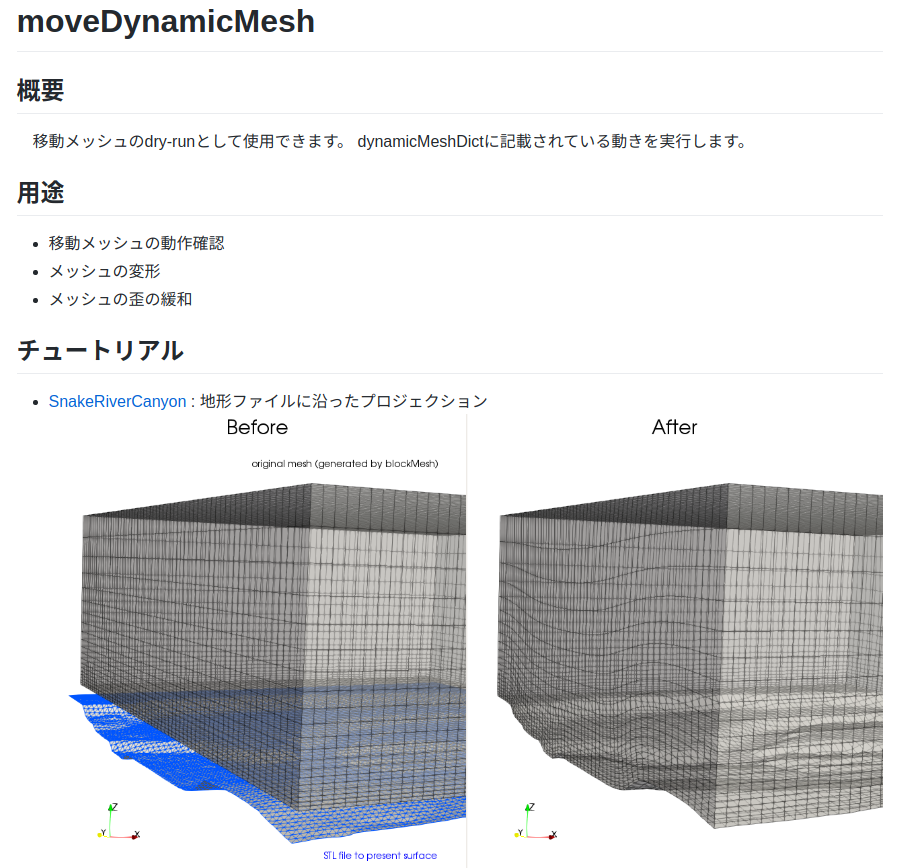
\includegraphics[width=0.8\textwidth]{fig/utilities-example.png}
\caption{moveDynamicMesh(v1906) utilitiy's tutorial document.\cite{URL:OpenFOAM-jp-movedDynamicMesh}}
\label{fig:utilities-example}
\end{figure}
各utilityについて,使用方法をMarkDown形式のドキュメントでまとめ,そのチュートリアルを作成する.
ディレクトリ構成は実際のソースコードに準拠し,最表層のMarkDownファイルから各ドキュメントにアクセスできるようにしている.\cite{URL:OpenFOAM-jp-util-index}
現時点ではOpenFOAM-v1906について作成中である.
%
\section{まとめ}

%%%
%%% OpenCAEシンポジウムTeXテンプレートファイル
%%% OpenFAOM-jp_OpenCAE_symposium.tex
%%% OpenCAEシンポジウム2018版
%%%
%%
%% ltjocはOpenCAE論文集・シンポジウム用のクラスファイルです.変更しないでください.
%% 本文が英語の場合には,オプションにenglishを指定してください.
\documentclass{ltjoc}
%\documentclass[english]{ltjoc}
\usepackage[
 backgroundcolor=gray!50,
 usernamecolor=black,
 machinenamecolor=black,
 indicatorcolor=black,
 separatorcolor=black,
 pathcolor=black,
 optioncolor=black,
 textcolor=black
]{shdoc}
%%
%% 表題(title),副題(subtitle),著者(author),所属(affiliation)
%% 本文が英語の場合には,こちらに英文表題,英文副題,英文著者,英文所属を記述します.
\title{OpenFOAMコントリビュート活動}
% 副題が無い場合にはコメントアウトします.
% \subtitle{\TeX のテンプレート(和文副題)} 
\author{%
稲葉竜一$^{1\dagger}$%
\hspace{1\zw}%
松原 大輔$^{2}$%
\hspace{1\zw}%
@tkoyama010$^{1}$%
}
\affiliation{%
${}^{1}$OpenFOAM-jp%
\hspace{1\zw}%
${}^{2}$オープン CAE勉強会%
} 
%%
%% Corresponding authorの電子メールアドレス
%% 本論文について連絡が取れる著者の電子メールアドレスを記載してください.
\AuthorsEmail{inabower@gmail.co.jp}
%%
%% 英文表題(etitle),英文副題(esubtitle),英文著者(eauthor),英文所属(eaffiliation)
%% 本文が英語の場合には表示されません.
\etitle{OpenFOAM Contributing Activities}
% 副題が無い場合にはコメントアウトします.
% \esubtitle{The case of \TeX (English Sub-Title)}
\eauthor{%
Ryuichi INABA$^{*\dagger}$%
\hspace{1em}%
Daisuke MATSUBARA$^{**}$%
\hspace{1em}%
@tkoyama010$^{*}$%
}
\eaffiliation{%
${}^{*}$OpenFOAM-jp%
\hspace{1em}%
${}^{**}$OpenCAE Local user group%
}
%%
%% キーワード
\keywords{GitHub, git, Pull Request, OpenFOAM, develop}
%%
%% 英文概要
%% 英文概要を省略する場合には,abstract環境の定義をしないでください.
\begin{abstract}
Commits from Japanese to OpenFOAM are less.
So, we established a group called OpenFOAM-jp by volunteers.
We started contributing activities such as development of software,
translation of documents and preparation of tutorials.
We will report how to join our activity by using git and GitHub.
\end{abstract}
%%
%% luatexja-fontspecパッケージ
\usepackage{luatexja-fontspec}
\defaultfontfeatures{Ligatures=TeX}
%% luatexja-presetパッケージ
%% 和文フォントのプリセット設定
%% オプションにnoembed(非埋込)を指定しないでください.
%\usepackage[ipaex]{luatexja-preset} % IPAex(デフォルト)
%\usepackage[ms]{luatexja-preset} % MS
%\usepackage[hiragino-pro]{luatexja-preset} % ヒラギノPro
%%
%% 欧文フォントの指定
%% 使用できるフォントについては,以下のコマンドで調べてください.
%% $ luaotfload-tool --list=*
%%
%% 欧文通常フォント
%\setmainfont{Cambria} % Cambria
%\setmainfont{Times New Roman} % Times New Roman
%\setmainfont{TeXGyreTermes} % TeXGyreTermes
%%
%% 欧文Sans-serifフォント
%\setsansfont{Calibri} % Calibri
%\setsansfont{Arial} % Arial
%\setsansfont{Helvetica} % Helvetica
%\setsansfont{TeXGyreHeros} % TeXGyreHeros
%%
%% 欧文monospaceフォント
%\setmonofont{Consolas} % Consolas
%\setmonofont{Courier New} % Courier New
%\setmonofont{Lucida Console} % Lucida Console
%%
%% subfigureパッケージ
\usepackage{subfigure}
%%
%% graphicxパッケージ
\usepackage{graphicx}
%%
%% hyperrefパッケージ
\usepackage[
 pdfencoding=auto,
 bookmarks=true,
 bookmarksnumbered=true,
 colorlinks=true,
 allcolors={blue}
]{hyperref}
%%
%% listingsパッケージ
\usepackage{listings}
\renewcommand{\lstlistingname}{Code}
\lstset{
basicstyle={\footnotesize\ttfamily},
commentstyle=\color{blue},
frame={tb},
breaklines=true,
columns=[l]{fullflexible},
numbers=left,
numberstyle={\footnotesize},
keepspaces=true
}
%%
%% autorefでの図表の参照名の再定義
\makeatletter
\if@english
  \renewcommand*{\figureautorefname}{\figurename}
  \renewcommand*{\tableautorefname}{\tablename}
\else
  \renewcommand*{\figureautorefname}{図}
  \renewcommand*{\tableautorefname}{表}
\fi
\makeatother
%%
%% ヘッダ右の設定
%% 変更しないでください.
\markright{Open CAE Symposium 2019, Dec. 19-21, 2019, Osaka, D-2} % Do not edit this line
%%
%% 本文
\begin{document}
%%
%% 題目などの出力
\maketitle
%%%
\section{はじめに}
現状日本からのOpenFOAMへのコントリビュートは少ない.
そこで有志により"OpenFOAM-jp"といグループを立ち上げ,本家の開発やドキュメントの翻訳,チュートリアルの作成などのコントリビュート活動を始めた.
本報告ではその活動内容などについて発表する.
\section{Foundation版とESI版の違い}
OpenFOAMは,Imperial Collageで開発された商用CFDコードFOAM(Field Operation And Manipulation)が,2004年にOpenFOAMと名前を変えてオープンソースとしてリリースされたことから始まる.\cite{URL:openfoam.history}\cite{Minabe:OpenCAE2015-GP23}
2011年にはOpenFOAMを運営しているOpenCFD社がSGI社に買収され,またその2社によりOpenFOAMの商標を譲渡したOpenFOAM Foundation Inc.を設立した.
これ以降OpenFOAMはOpenFOAM Foundation Inc.より開発と配布が行われており,2019年11月現在OpenFOAM-V7を最新版とするForkが”Foundation版”\cite{URL:openfoam.org}\cite{URL:GitHub-foundation}と呼ばれている.

一方でOpenFOAMには多くのForkが存在する.
2012年以降はESI社がOpenCFD社の買収という形から開発に加わるようになり,
2016年にはOpenFOAM-v3.0からForkしたOpenFOAM-v3.0+をリリースした.
2019年11月時点ではこの最新版はOpenFOAM-v1906であり,このForkが”ESI版”\cite{URL:openfoam.com}\cite{URL:GitLab-plus}もしくは”plus版”と呼ばれる.

本報告ではこのFoudation版とESI版の2つについてコントリビュートの流れなどを報告する.
%
\section{ESI版コントリビュート方法}
ESI版の開発はGitLabで行われている.\cite{URL:GitLab-plus}
このページからレポジトリをcloneすることができ,これをそのままコンパイルすることで次期リリース予定のESI版OpenFOAMを使用することができる.
またここには開発途中のbranchが多くあり,将来的に追加されるであろう機能をチェックすることもできる.

\autoref{fig:plus-register}に示すGitLabのページの右上のボタンからこのOpenFOAM-plusのレポジトリに登録することもでき,これによりissueの作成や書き込みをすることができるようになる.
\begin{figure}[htbp]
\centering
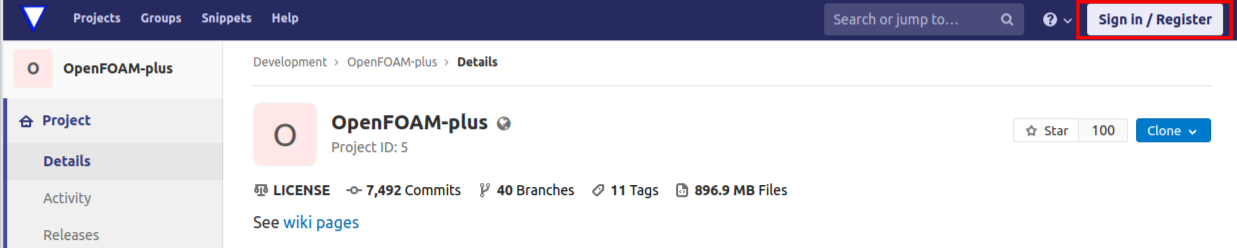
\includegraphics[width=0.8\textwidth]{fig/plus_register.png}
\caption{A register button of OpenFOAM-plus's GitLab page.}
\label{fig:plus-register}
\end{figure}
例えばバグを見つけた場合やOpenFOAMへの要望がある場合には,issueを作成することで開発者へ周知することができ,必要と判断された場合には開発者によりコードの修正や作成が行われる.
\autoref{fig:plus-issue}には実際に作成したissueの例を示す.内容としてはソルバーのDiscriptionの中のスペルミスを指摘した簡単なものであるが,数日以内に@mark氏により該当箇所の修正が行われていることが確認できる.
\begin{figure}[htbp]
\centering
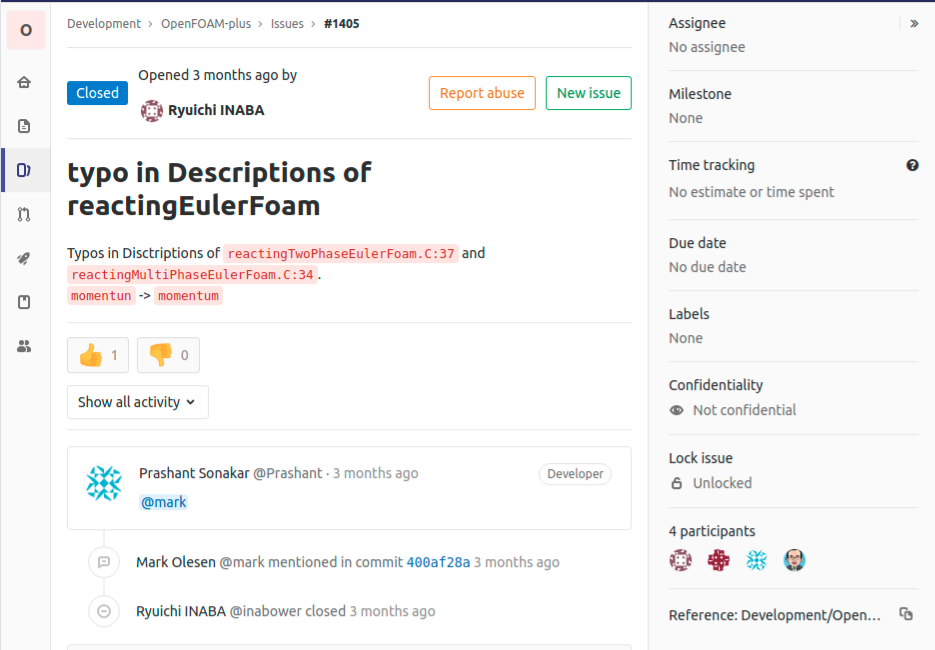
\includegraphics[width=0.8\textwidth]{fig/plus_issue.png}
\caption{An Example issue to fix typo.}
\label{fig:plus-issue}
\end{figure}
このような小さなコントリビュートの積み重ねがOSSであるOpenFOAMを精錬していくこととなる.

一方で,pushやPull Requestなどのコードの変更を行うための権限は制限されている.
このため,ESI版OpenFOAMのコードにコントリビュートする手段としては,開発メンバーに加わらない限りはissueの作成もしくはissue内の議論へ参加することに限られる.
なお2019年11月現在OpenFOAM-plusの開発メンバーは15名であり,実力や面識,貢献頻度が担保されたメンバーで開発を行っていることが推察される.\cite{URL:GitLab-plus-members}
%
\section{Foundation版コントリビュート方法}

Foundation版の開発はGithubで行われている.Foundation版ではissueの管理はGithubでは行わないので注意が必要である.バグ報告は専用のissueTrackingのページへ登録する必要がある.
未登録の場合は,名前とメールアドレスを入力し,返信のリンクを辿ることでviewerとして参加することができる.
また数時間後にスパムでないことが認められると,reporterに昇格できる.
reporterとなることでissueを立てて,バグの報告が可能となる.
ここでバグの重要度や改善方法を議論をすることになる.
issueTrackingの内容を確認すると,Foundation版は基本的にbugfixを目的としたコントリビュートが主の様である.

重大なバグの修正または,新しい開発を提供する場合,OpenFOAM Foundation Contributor Agreementに署名する必要がある.
Foundation版HPのメニューバーのDevelopment/ContributorAgreeementのリンクを辿り,Contact Usのページから名前と所属,コントリビュートに参加した意思を記載して送信すると,後日,Henry G. WellerからPDF形式の登録用紙が送付されてくる.
登録用紙の内容は,前述のContributorAgreeementのページに記載されているものと同じである.

バグの修正などでFoundation版のOpenFOAMの修正を開発元に共有する場合,Foundation版のOpenFOAMはgithub上で管理されているため,githubアカウントが必要となる.

コントリビュートで最初に行うことは開発元のリポジトリをForkすることから始まる.(\autoref{fig:f1})
Forkしたことにより,自身のgithubアカウントにOpenFOAMのリポジトリが作成されていることが確認できる.
次に開発用の新しいブランチを作成する.ブランチ名は「(開発者名)-patch***」などとするとよいだろう.今回の例では「matsubara-patch1」とした.(\autoref{fig:f2})

\begin{figure}[htbp]
\centering
\subfigure[A fork button of Github page]{
  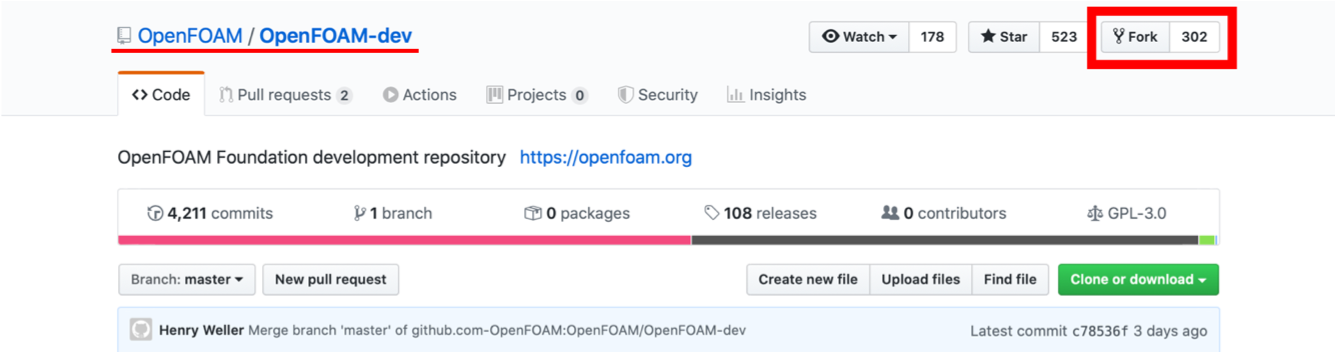
\includegraphics[width=0.8\textwidth]{fig/fig-f1.png}
  \label{fig:f1}
}
%\hspace{0.1\textwidth}
\subfigure[Creating new branch]{
  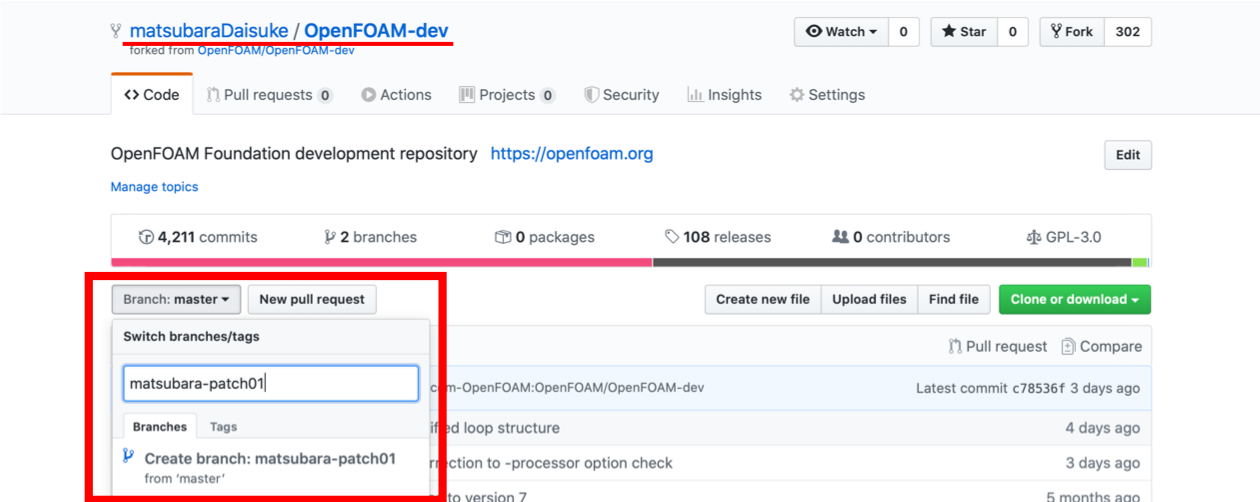
\includegraphics[width=0.8\textwidth]{fig/fig-f2.png}
  \label{fig:f2}
}
\caption{A Explication to fork OpenFOAM-dev repository and to create your new branch.}
\label{fig:f1f2}
\end{figure}
%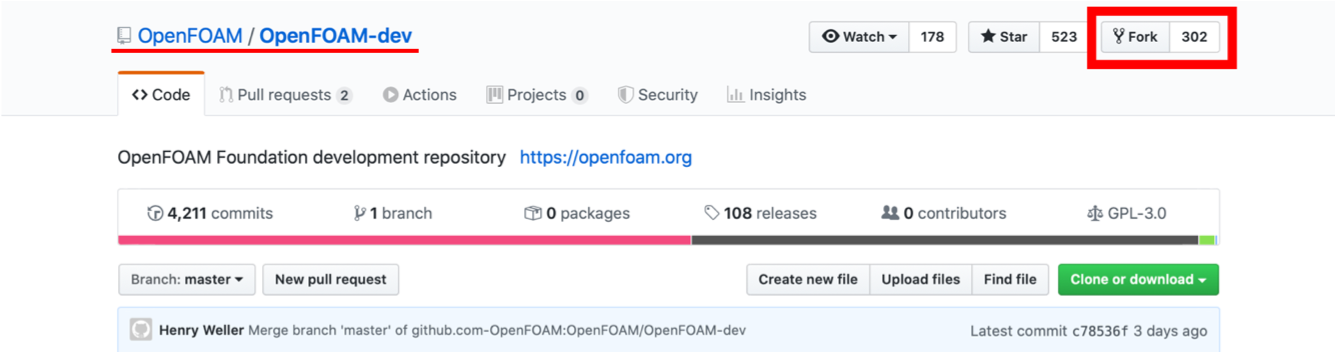
\includegraphics[width=5cm]{fig/fig-f1.png}
%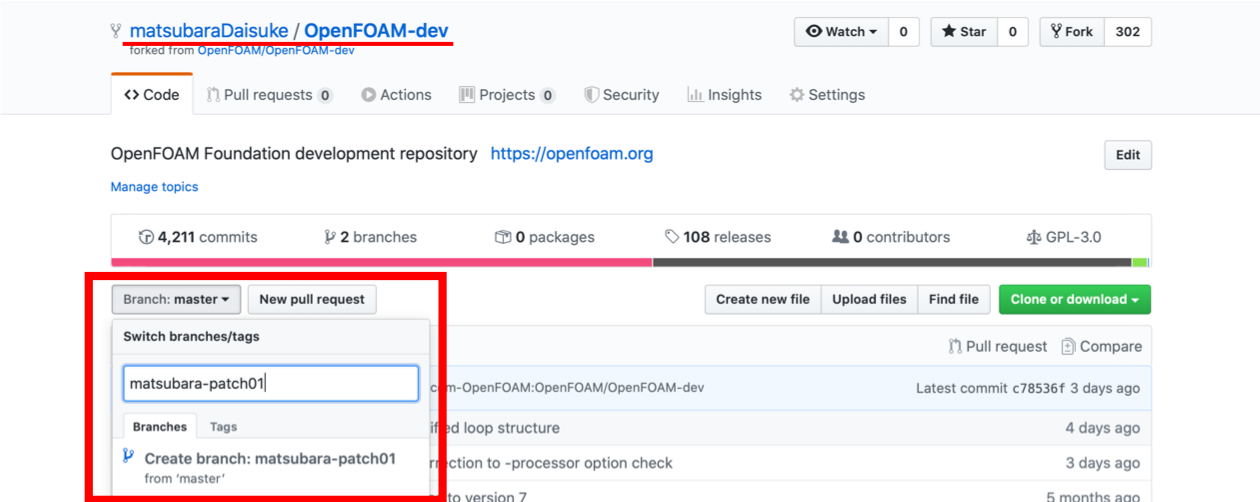
\includegraphics[width=5cm]{fig/fig-f2.png}

次に個人の開発環境に移りターミナル上でgit cloneを行う.(\autoref{fig:f3})例:git clone https://github.com/(githubアカウント名)/OpenFOAM-dev.git
これによって,git cloneしたディレクトリ下にOpenFOAMのプロジェクトがコピーされる.
%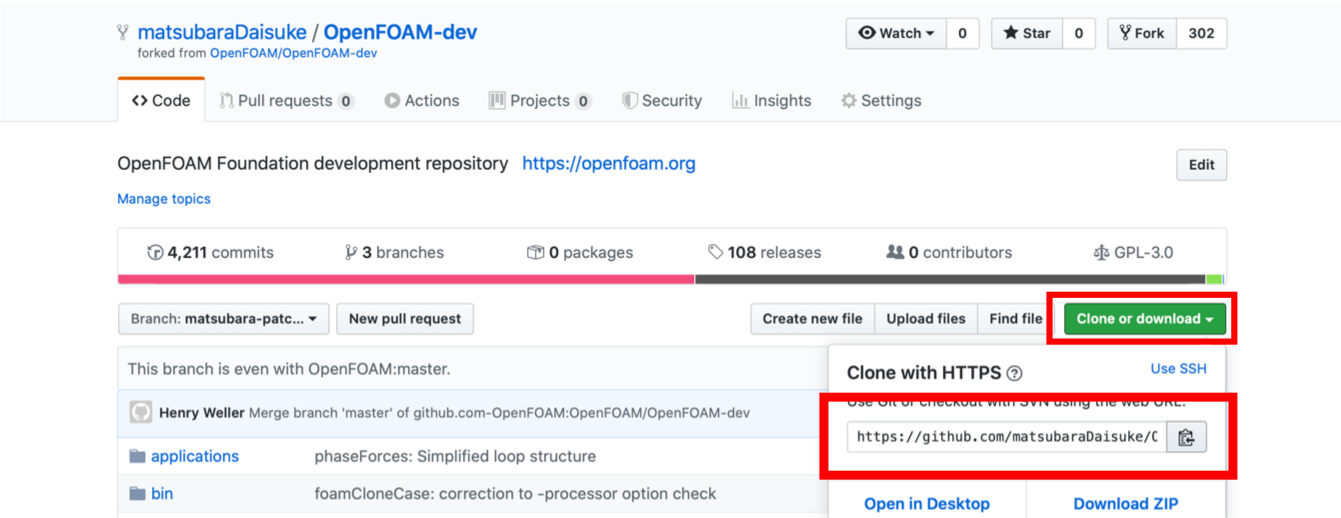
\includegraphics[width=5cm]{fig/fig-f3.png}
\begin{figure}[htbp]
\centering
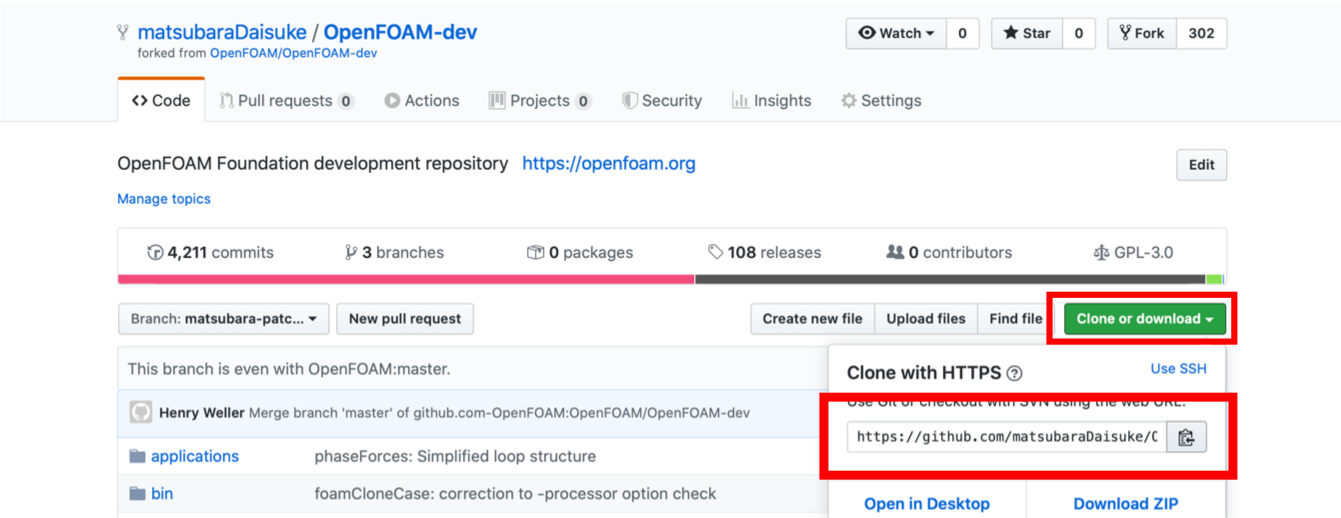
\includegraphics[width=0.8\textwidth]{fig/fig-f3.png}
\caption{Cloning repository on your local machine.}
\label{fig:f3}
\end{figure}

次にgit checkoutにて作成したブランチに切り替える 例:git checkout (開発者名)-patch***
OpenFOAMのプロジェクト内で修正や開発が完了した後,
git add . git commit -m "変更内容のコメント" git push origin (開発者名)-patch***
とすることで,コードの修正内容を個人のgithubのリポジトリに反映させる.
今回の例では以下の様な流れになる.

\begin{shbox}
  \shuser{user}
  \shline{}{git clone https://github.com/matsubaraDaisuke/OpenFOAM-dev.git}  
  \shline{}{cd OpenFOAM-dev}  
  \shline{}{git checkout matsubara-patch1}
\end{shbox}

(コーディング)

\begin{shbox}
  \shuser{user}
  \shline{}{git add .}
  \shline{}{git commit -m "bugfix ******"}
  \shline{}{git push origin matsubara-patch1}
\end{shbox}



最後にgithub上でpull requestを開発元に対して行う.(\autoref{fig:f4})この時コメントに
Fixes issue:
https://bugs.openfoam.org/view.php?id=****
の様に最初に議論したissueのURLを添付するのが慣例のようである.(\autoref{fig:f5})

%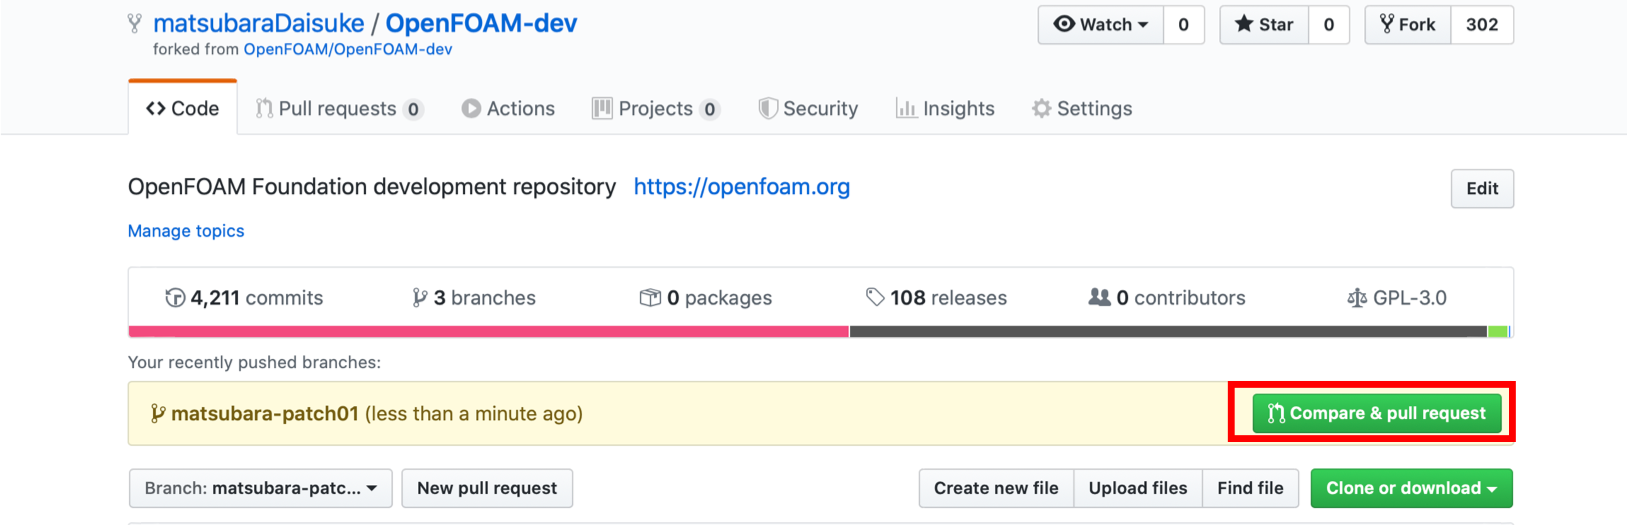
\includegraphics[width=5cm]{fig/fig-f4.png}
%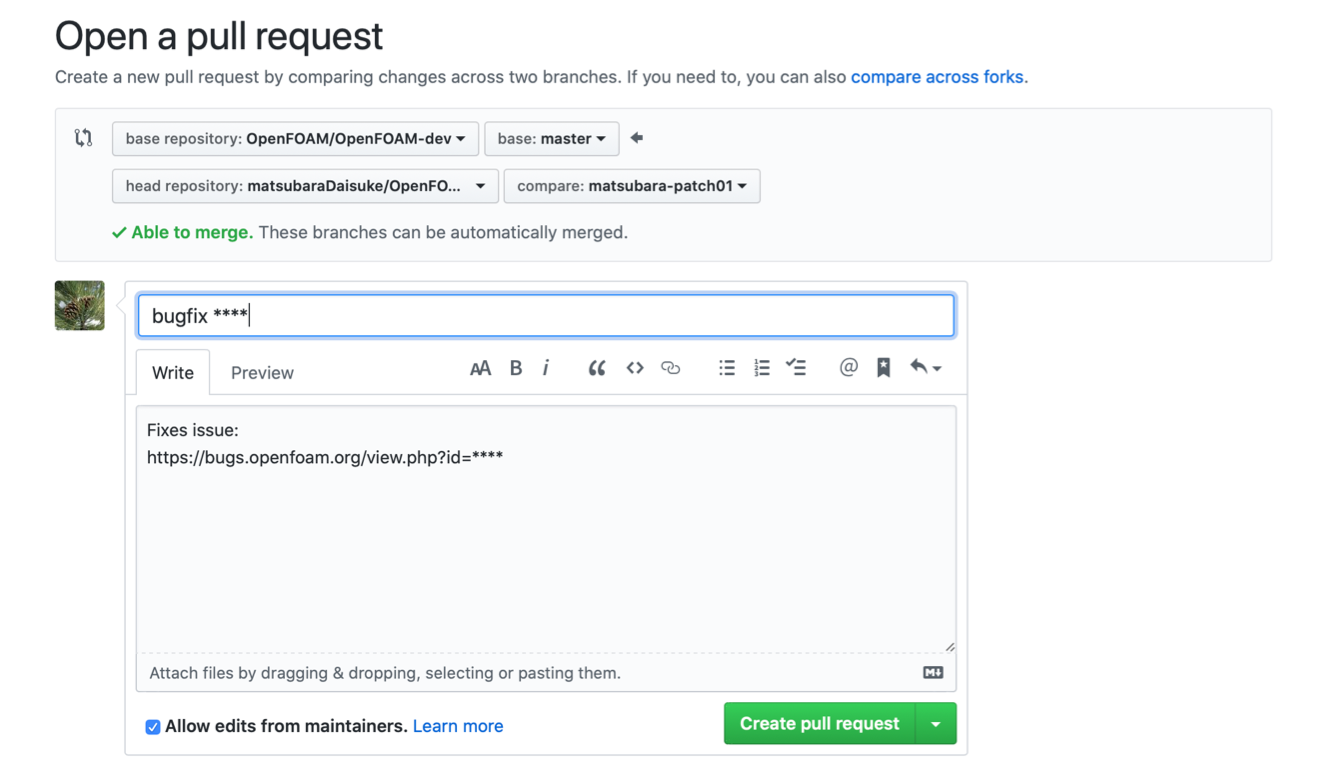
\includegraphics[width=5cm]{fig/fig-f5.png}
\begin{figure}[htbp]
\centering
\subfigure[Pull request your branch into the master branch.]{
  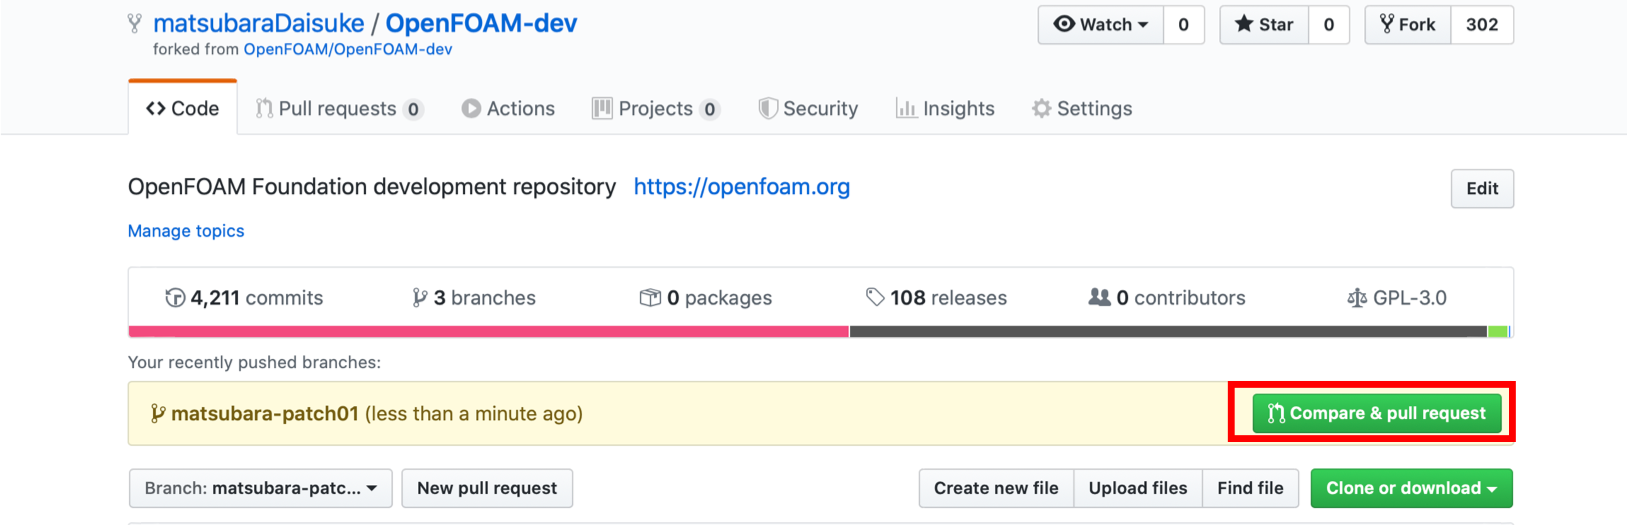
\includegraphics[width=0.8\textwidth]{fig/fig-f4.png}
  \label{fig:f4}
}
%\hspace{0.1\textwidth}
\subfigure[Add your message to pull request.]{
  \includegraphics[width=0.8\textwidth]{fig/fig-f5.png}
  \label{fig:f5}
}
\caption{A explication to pull request your branch into the master branch.}
\label{fig:f4f5}
\end{figure}


\section{Gitの使い方}
本節では https://github.com/OpenFOAM-jp/OpenFOAM-jp.git 
のリポジトリにコントリビュートの練習をする方法について解説する.
環境はUbuntu18.04の環境を想定する.
事前に{GitHub}のアカウントを作成する必要がある.
コントリビュートをする際にはまず,Issueを立て自分が加えたい変更について議論する.
Issueを立てる際には以下の内容が含まれていることが望ましい.
\begin{itemize}
  \item 機能の簡単な説明.問題が何であるかの明確で簡潔な説明.
  \item 希望するソリューションの説明.あなたが何をしたいのかについての明確で簡潔な説明.
  \item 検討した代替案を説明.検討した代替ソリューションまたは機能の明確で簡潔な説明.
  \item 追加のコンテキスト.機能リクエストに関する他のコンテキストまたはスクリーンショットをここに追加します.
\end{itemize}
OSSのコントリビュートのバージョン管理ソフトにはGitが一般的に使用されている.
OpenFOAMの開発においてもGitが使用されている.
まずは,Gitをインストールする.

\begin{shbox}
  \shuser{user}
  \shline{}{sudo apt install git}
\end{shbox}

必要なのはソースだけで貢献しないのであれば,次のコマンドでcloneすることで作業は終わる.

\begin{shbox}
  \shuser{user}
  \shline{}{git clone https://github.com/OpenFOAM-jp/OpenFOAM-jp.git}
\end{shbox}

貢献をしたい場合は,OpenFOAM-jpのリポジトリを自分のアカウントにForkする.

TODO: Forkの際の画面キャプチャを挿入する.

Fork後は自分のアカウントのリポジトリをcloneする.

\begin{shbox}
  \shuser{user}
  \shline{}{git clone https://github.com/your\_account\_name/OpenFOAM-jp.git}
\end{shbox}

cloneをしたら自分の環境で実行環境を構築する.
まずは,OpenFOAMを動かすために必要な外部ライブラリをインストールする.

\begin{shbox}
  \shuser{user}
  \shline{}{sudo apt update}
  \shline{}{sudo apt upgrade}
  \shline{}{sudo apt install git-core}
  \shline{}{sudo apt install build-essential}
  \shline{}{sudo apt install cmake}
  \shline{}{sudo apt install libfl-dev}
  \shline{}{sudo apt install bison}
  \shline{}{sudo apt install zlib1g-dev}
  \shline{}{sudo apt install qt4-dev-tools}
  \shline{}{sudo apt install libqt4-dev}
  \shline{}{sudo apt install libqtwebkit-dev}
  \shline{}{sudo apt install gnuplot}
  \shline{}{sudo apt install libreadline-dev}
  \shline{}{sudo apt install libncurses-dev}
  \shline{}{sudo apt install libxt-dev}
  \shline{}{sudo apt install libopenmpi-dev}
  \shline{}{sudo apt install openmpi-bin}
  \shline{}{sudo apt install libboost-system-dev}
  \shline{}{sudo apt install libboost-thread-dev}
  \shline{}{sudo apt install libgmp-dev}
  \shline{}{sudo apt install libmpfr-dev}
  \shline{}{sudo apt install python}
  \shline{}{sudo apt install python-dev}
  \shline{}{sudo apt install libcgal-dev}
  \shline{}{sudo apt install curl}
  \shline{}{sudo apt install git-core}
  \shline{}{sudo apt install build-essential}
  \shline{}{sudo apt install cmake}
  \shline{}{sudo apt install libfl-dev}
  \shline{}{sudo apt install bison}
  \shline{}{sudo apt install zlib1g-dev}
  \shline{}{sudo apt install qt4-dev-tools}
  \shline{}{sudo apt install libqt4-dev}
  \shline{}{sudo apt install libqtwebkit-dev}
  \shline{}{sudo apt install gnuplot}
  \shline{}{sudo apt install libreadline-dev}
  \shline{}{sudo apt install libncurses-dev}
  \shline{}{sudo apt install libxt-dev}
  \shline{}{sudo apt install libopenmpi-dev}
  \shline{}{sudo apt install openmpi-bin}
  \shline{}{sudo apt install libboost-system-dev}
  \shline{}{sudo apt install libboost-thread-dev}
  \shline{}{sudo apt install libgmp-dev}
  \shline{}{sudo apt install libmpfr-dev}
  \shline{}{sudo apt install python}
  \shline{}{sudo apt install python-dev}
  \shline{}{sudo apt install libcgal-dev}
  \shline{}{sudo apt install curl}
\end{shbox}

次に,OpenFOAMのbashrcをターミナル起動時に読み込むように~/.bashrcに登録する.

\begin{shbox}
  \shuser{user}
  \shline{}{echo "source ~/OpenFOAM/OpenFOAM-dev/etc/bashrc" >> ~/.bashrc}
  \shline{}{. ~/.bashrc}
\end{shbox}

ThirdPartyの中のParaViewをインストールする.
この際にpythonを登録するとParaViewのpython拡張機能が使用可能になる.
既にParaViewをインストールしている場合であっても,このParaViewはOpenFOAMの結果表にのプラグインなども同梱しているため,
以下の手順でもう一つインストールすることを推奨する.

\begin{shbox}
  \shuser{user}
  \shline{}{cd \$WM\_THIRD\_PARTY\_DIR}
  \shline{}{./makeParaView -python -python-lib /usr/lib/x86\_64-linux-gnu/libpython2.7.so.1.0}
\end{shbox}

最後にOpenFOAMをインストールする.

\begin{shbox}
  \shuser{user}
  \shline{}{wmRefresh}
  \shline{}{cd \$WM\_PROJECT\_DIR}
  \shline{}{./Allwmake -j | tee log.Allwmake}
\end{shbox}

ソルバーを動かしてインストールの確認を行う.

\begin{shbox}
  \shuser{user}
  \shline{}{mkdir \$WM\_PROJECT\_USER\_DIR}
  \shline{}{cd \$WM\_PROJECT\_USER\_DIR}
  \shline{}{cp -r \$FOAM\_TUTORIALS/basic/potentialFoam/pitzDaily/ ./}
  \shline{}{cd pitzDaily/}
  \shline{}{foamRunTutorials}
  \shline{}{paraFoam}
\end{shbox}

これでParaViewが起動されて結果の表示ができたら完成である.
テストが全てパスしたらソースを変更する.
masterブランチで直接変更することはできないため,ファイルを変更する前に開発ブランチを作成する.

\begin{shbox}
  \shuser{user}
  \shline{}{git branch branch\_name}
\end{shbox}
\begin{shbox}
  \shuser{user}
  \shline{}{git checkout branch\_name}
\end{shbox}

branch\_name には任意の名前を入れる.
自分のアカウント名と加えたい変更について言及されていると分かりやすい.
最初のコマンドでブランチを作成し,2番目のコマンドでブランチに移動する.
これにより,変更を行う準備はほぼ完了である.
変更のラベルを付けるために,連絡先の名前と電子メールを以下のコマンドで指定する.

\begin{shbox}
  \shuser{user}
  \shline{}{git config --global user.name "Your Name Comes Here"}
  \shline{}{git config --global user.email you@yourdomain.example.com}
\end{shbox}

もし src/toto.cc というファイルをいくつか変更したり,新しいファイルとして追加したら,
ローカルのコミットは次のコマンドで行う.
"Your extensive commit message here \#1" には変更に関するメッセージを追加する.
\#1の部分は自分が追加したイシューの番号とする.

\begin{shbox}
  \shuser{user}
  \shline{}{git add src/toto.cc}
  \shline{}{git commit -m "Your extensive commit message here \#1"}
\end{shbox}

この段階ではコミットはあなたのローカルリポジトリで行われていますが,GitHubリポジトリでは行われない.
十分なテストで変更を検証したら,以下のコマンドでGitHubの自分のアカウントのリポジトリに変更を移すことができる.

\begin{shbox}
  \shuser{user}
  \shline{}{git push origin branch\_name}
\end{shbox}

TODO: コマンドのメッセージを含める

このコマンドのメッセージに図のようなURLが表示される.
URLにアクセスしプルリクエストを作成する.

TODO: GetFEMのドキュメントから引用を行っているため言及する.

GetFEM++ のマスターブランチにマージすることは許可されていないので,あなたの役割はここで終わる.
プルリクエストのページで管理者や他の開発者と議論することができる.
管理者が承認した場合には変更がマージされる.

いくつかの便利なgitコマンドを示す.

\begin{shbox}
  \shuser{user}
  \shline{}{git status  : status of your repository / branch}
  \shline{}{git log --follow "filepath"   : Show all the commits modifying the specified file (and follow the eventual change of name of the file).}
  \shline{}{gitk --follow filename : same as previous but with a graphical interface}
\end{shbox}

\section{GitHub および Travis による継続的インテグレーション}
Travis CIは,GitHub上のソフトウェアのビルドやテストを行う,オンラインで分散型の継続的インテグレーション (CI) サービスである.
継続的インテグレーションサービスとは,ビルドやテストを継続的に自動実行するサービスである.
継続的インテグレーションを行うことにより,機能追加やリファクタリングによるデグレードを防ぐことができる.
以下に,GetFEM++で使用している.travis.ymlを示す.
リポジトリにymlファイルを追加することで,Travisによるインテグレーションテストが実行される.
今後OpenFOAMのリポジトリでもCIが実行できるようにする予定である.
\begin{lstlisting}
language: python
python:
  - "3.6"
sudo: false
dist: bionic
cache:
  directories:
  - $HOME/.cache/pip
before_install:
- sudo apt-get install -y --no-install-recommends automake
- sudo apt-get install -y --no-install-recommends libtool
- sudo apt-get install -y --no-install-recommends make
- sudo apt-get install -y --no-install-recommends g++
- sudo apt-get install -y --no-install-recommends libqd-dev
- sudo apt-get install -y --no-install-recommends libqhull-dev
- sudo apt-get install -y --no-install-recommends libmumps-seq-dev
- sudo apt-get install -y --no-install-recommends liblapack-dev
- sudo apt-get install -y --no-install-recommends libopenblas-dev
- sudo apt-get install -y --no-install-recommends libpython3-dev
- sudo apt-get install -y --no-install-recommends ufraw
- sudo apt-get install -y --no-install-recommends imagemagick
- sudo apt-get install -y --no-install-recommends fig2dev
- sudo apt-get install -y --no-install-recommends texlive
- sudo apt-get install -y --no-install-recommends xzdec
- sudo apt-get install -y --no-install-recommends fig2ps
- sudo apt-get install -y --no-install-recommends gv
- pip install -r requirements.txt
addons:
  apt:
    update: true
script:
- bash autogen.sh
- export CXXFLAGS=-coverage
- export LDFLAGS=-coverage
- export CPPFLAGS=-coverage
- export CFLAGS=-coverage
- export FCFLAGS=-coverage
- ./configure --with-pic
- make -j8
- make -j8 check
- (cd doc/sphinx; make html)
after_success:
- bash <(curl -s https://codecov.io/bash)
\end{lstlisting}

TODO Travis CIについてWikipediaからの引用であることを明記する.

TODO 継続的インテグレーションサービスについてWikipediaからの引用であることを明記する.
%
\section{OpeFOAM-jp}
OpenFOAM-jp\cite{URL:OpenFOAM-jp}は今回立ち上がったコミュニティの活動を行うためのGiuHubレポジトリである.
目的は日本のOpenFOAMコミュニティの活性化,OpenFOAMへのコントリビュートの入り口,およびOSSコントリビュート活動の学習の場としている.
参加は誰でも国籍を問わず可能であり,今後人口が増えてオープンで有意義な場として機能することを期待する.
%
\subsection{OpenFOAM-jp/issues}
issuesレポジトリ\cite{URL:OpenFOAM-jp-issues}は最初の議論を行う場として設置された.
テキストエディタVimの日本コミュニティのレポジトリ\cite{URL:vim-jp}のForkであり,運用方法もこれを参考にする.
ここではOpenFOAMの新機能の提案やOpenFOAM-jpで行う活動の議論などを行うことを目的としている.
質問掲示板であるGoogle Forumと役割が重複すると混乱や情報の偏りを発生させるため明確な差別化を行うように注意して運用していく.
%
\subsection{OpenFOAM-jp/OpenFOAM-jp}
OpenFOAM-jpレポジトリ\cite{URL:OpenFOAM-jp-OpenFOAM-jp}はFoundation版のOpenFOAM-devのForkであり,pushやPull Requestなどのgitの基本機能の練習用に設置された.
branchを作成してオリジナルの機能を配布する目的で使用することも期待している.
エラーメッセージの日本語化プロジェクトなども予定している.
%
\subsection{OpenFOAM-jp/OpenFOAM-utilities-tutorials-jp}
OpenFOAM-utilities-tutorials-jp\cite{URL:OpenFOAM-jp-OpenFOAM-utilities-tutorials-jp}は,web上にあまり情報のないOpenFOAMのutilitiesに関するまとめを行う目的で設置された.
その一例を\autoref{fig:utilities-example}に示す.
\begin{figure}[htbp]
\centering
\includegraphics[width=0.8\textwidth]{fig/utilities-example.png}
\caption{moveDynamicMesh(v1906) utilitiy's tutorial document.\cite{URL:OpenFOAM-jp-movedDynamicMesh}}
\label{fig:utilities-example}
\end{figure}
各utilityについて,使用方法をMarkDown形式のドキュメントでまとめ,そのチュートリアルを作成する.
ディレクトリ構成は実際のソースコードに準拠し,最表層のMarkDownファイルから各ドキュメントにアクセスできるようにしている.\cite{URL:OpenFOAM-jp-util-index}
現時点ではOpenFOAM-v1906について作成中である.
%
\section{まとめ}

\input{OpenFOAM-jp_OpenCAE_symposium.bbl}
\end{document}

\end{document}

\end{document}

\end{document}
